\chapter{Handling of trimuon correlations at LHCb}
\label{chap:trimuon}


\textit{This chapter discuss issues associated with three muons passing through the detector. Two collimated muons may traverse through the same parts of the detector if they have the same charge, causing problems in resolving their individual tracks. Therefore, ghosts and clones are much more likely to occur. In LHCb, a plethora of muon \Gls{PID} variables are used to suppress these types of spurious tracks. However, the usage of \gls{PID} variables in an analysis in \gls{LHCb} brings its own challenges. As the simulation is not able to estimate \gls{PID} efficiencies correctly, most of the \gls{PID} efficiencies are taken from control samples. New control samples for \Bmumumu are considered as the \Gls{PID} efficiencies depend strongly onthe number of muons in the detector and in the standard misID control samples there is just a single muon in each event.}

\color{black}

\section{Muon PID variables}
\label{otherpid}
In addition to the muon identification variables mentioned in~\autoref{muonID}, there is a further set of criteria for selecting muons. In this section a summary of the variables used in the analysis of the \Bmumumu is discussed.

\subsection{Binary Muon PID variables }
Similar to \texttt{isMuon} shown in~\autoref{tab:ismuontab}, there are more binary variables, such as \texttt{isMuonTight}, that can help with classification of muons. As its name suggests, \texttt{isMuonTight} has stronger conditions to satisfy as compared to \texttt{isMuon}. 

In each muon station (\gls{muonstation}) a field of interest, \gls{FOI} is defined as %a function of momentum $p$ in a following way:
\begin{equation}
	FOI_{x,y}=\rho^{0}_{x,y}+\rho^{1}_{x,y}\cdot \exp \left(\frac{\rho^{2}_{x,y}\cdot p}{\gevc} \right),
\end{equation}
where $x,y$ are the dimensions perpendicular to the direction of the beam, $p$ is momentum of the muon, $\rho^{i}_{x,y}$ are three dimension-dependent parameters tuned to give the best performance, by maximizing efficiency to misID rate.

When a muon passes through the detector, it leaves hits ($h_{x,y}$ coordinate) in a pad with size $pad_{x,y}$ of each muon station. From the tracks formed in the tracking part of the detector, coordinates $E_{x,y}$ are obtained by extrapolating the tracks into the muon stations. The hits are considered to be within the \gls{FOI} if they satisfy the condition that $|| h_{d} - E_{d} || < FOI_{d} \cdot pad_{d}$ for both d={x,y}. 

\color{black}

The detector information is read out in the $x$ and $y$ direction separately. The pad slicing according to this read-out scheme is known as \textit{physical} slicing of pads. However, as seen in~\autoref{fig:pads}, the overlapping $x$ and $y$ \textit{physical} pads can be grouped into \textit{logical} pads, which give information about $x$ and $y$ simultaneously. This leads to two groups of hits according to pad type: uncrossed hits - registered within \textit{physical} pads only, and crossed hits - given by \textit{logical} pads. Whereas \texttt{isMuon} only requires positive decision from uncrossed hits, \texttt{isMuonTight} requires positive decision based on crossed hits. 


\begin{figure}[!h]
        \centering
        %
\includegraphics[width = 0.3\textwidth]{figs/trimuon/poze.jpg}
        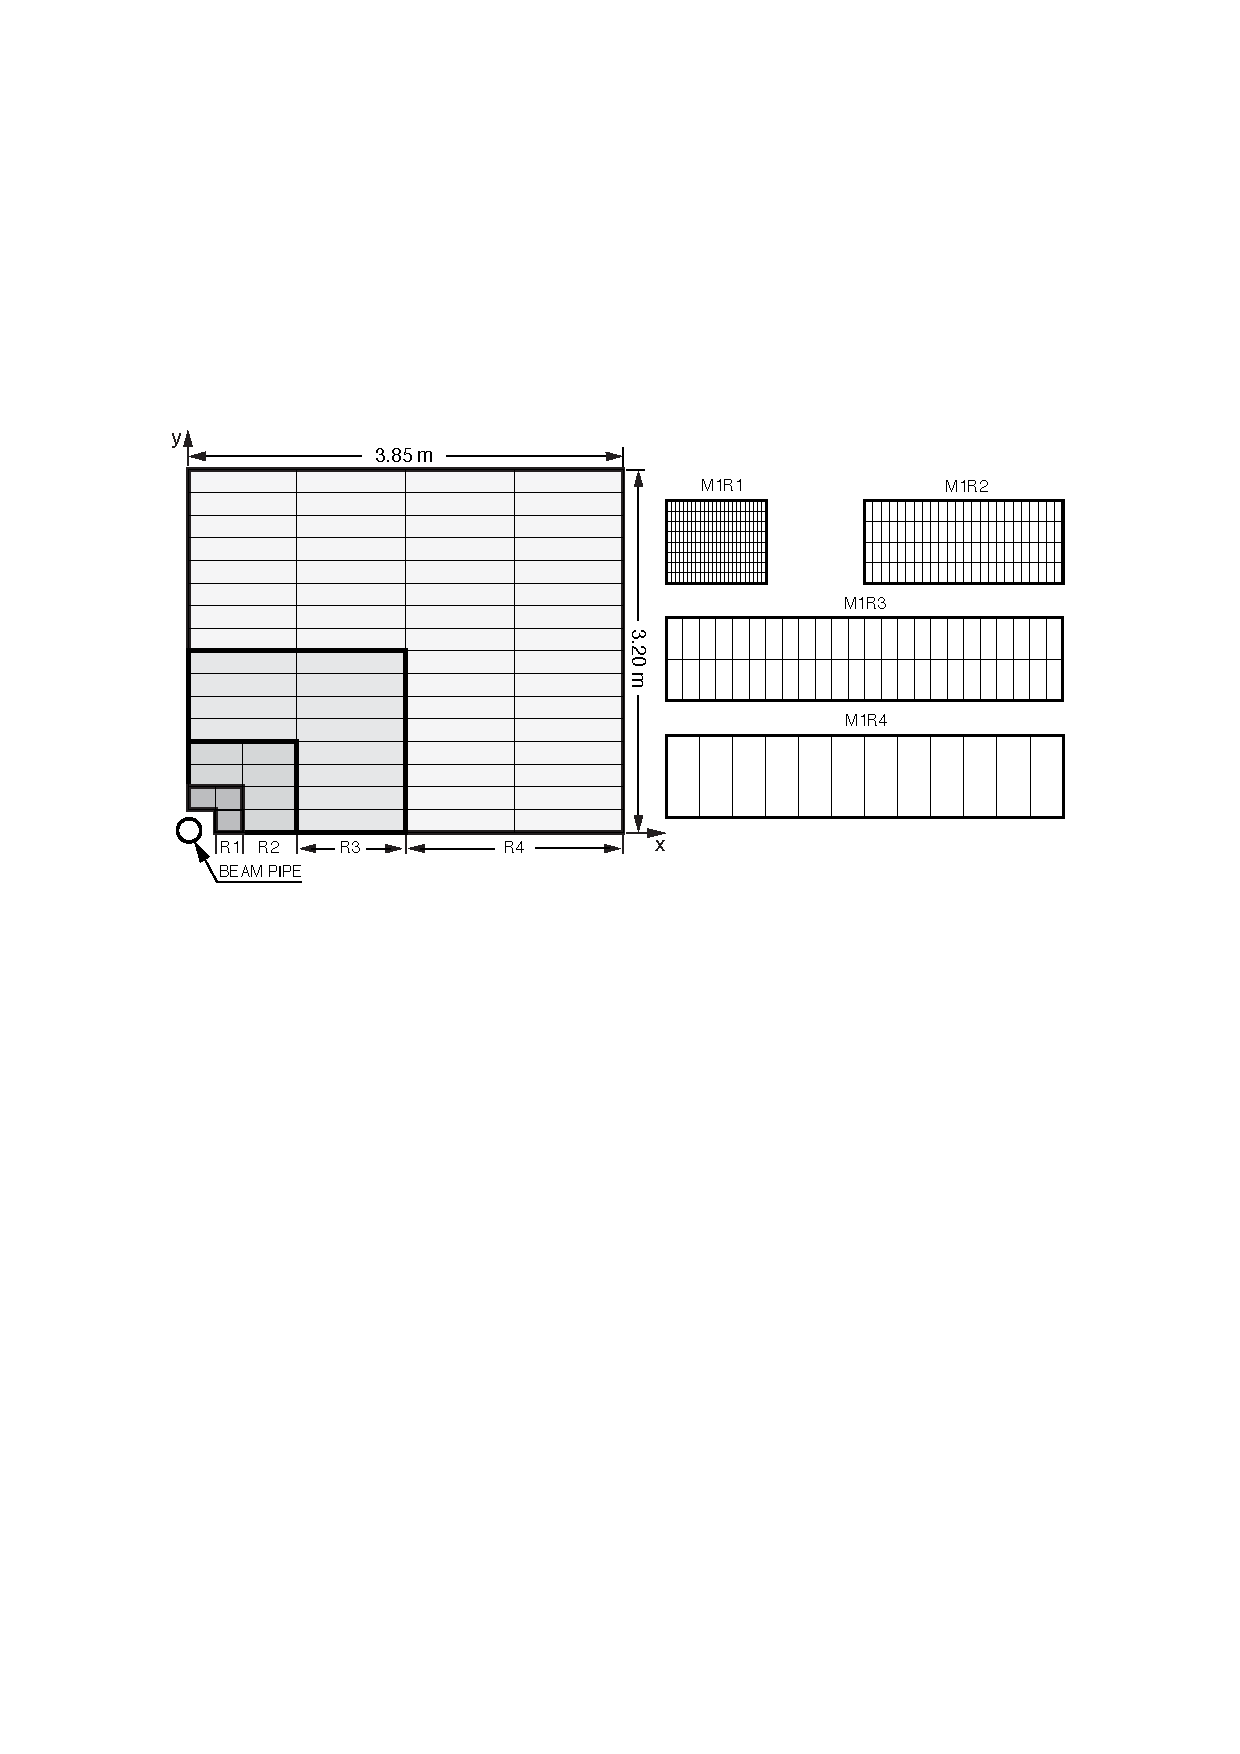
\includegraphics[width = 1.0\textwidth]{figs/trimuon/fig2.pdf}
        \caption{Schematic view of the muon station slicing into x-y pads. This is the left quadrant of the M1 station, showing decreasing granularity of the muon stations away from the beam pipe. This figure has been taken from \cite{LHCb-DP-2012-002}. M1R1 is the innermost region and M1R4 is the outermost region of the M1 station. }
        \label{fig:pads}
\end{figure}

\subsection{Muon PID variables based on sharing hits }
\label{bugs}

Another way of identifying muon tracks is based on the variable, \texttt{nShared}, which identifies the number of tracks with shared hits in the muon stations. For each hit within the \gls{FOI} of an extrapolated track, the \texttt{nShared} algorithm will check whether any other track was built using the given hit. In this case, the \texttt{nShared} variable of the muon track which has the bigger distance between the extrapolation coordinates and the hit coordinates is increased by 1. Hence this integer \gls{PID} variable helps suppressing \textit{ghost} tracks and \textit{clones} if no tracks have hits in common with the owner of the track (\texttt{nShared=0}).

%\subsection{Different \texttt{nShared} definitions for Run \Rn{1} and Run \Rn{2}
%To make sure that muons for \Bmumumu are not coming from these spurious tracks,  \texttt{nShared==0} for all three muons is required. These three muon tracks will not to share hits in muon stations with any other downstream or long tracks. In analysing data, there were features in the Muon ID alghorithm, software that calculates most of muon \gls{PID} variables, which changed between Run \Rn{1} and Run \Rn{2} and will be discussed in greater detail, as it impacts the selection performed for \Bmumumu search.
The muon identification software algorithms evolved significantly between the processing of Run \Rn{1} and Run \Rn{2} data. This included bug fixes, improvements and the introduction of new bugs. In the \Bmumumu analysis, this has to be taken into account.


The first feature that is different between Run \Rn{1} and Run \Rn{2} arises from the calculation of the distance between the extrapolation and the hit in \texttt{nShared} algorithm.
In \textit{Stripping 21} used for 2012 and \textit{21r1} used for 2011 data, it was discovered that the distance between an extrapolated track and a hit was wrongly calculated. This mistake was corrected before \textit{Stripping 23}, used for analysing 2015 data. 

Secondly, information from the M1 station was used to calculate distances, even though M1 information is not usually used for the Muon ID algorithms.  For analysts, this feature was present across all reconstruction software, meaning that simulation and data is affected in the same way.

In \textit{Stripping 23}, the Muon ID algorithm was rewritten to adapt to the parallelisation that needs to be done in order to meet the criteria for the upgrade of \gls{LHCb}. There were two mistakes introduced prior to 2015 data taking.
Firstly, an array was defined with 4-elements $[0,3]$ to store information about $x$ and $y$ coordinates of the hits. However, an iteration occurred by filling elements 1 to 4 of the array (M2-M5 station) resulting in a 5-element array where the 0-th element was not filled. Despite this, it turns out to be well-behaved and has no impact on physics.

Further in the process, however, this information is used to calculate the sum and average of distances per station between the hits and extrapolations. This algorithm again iterates over $[0,3]$ arrays, meaning that no information is used from the M5 muon station. This obviously has an effect, but again it is consistent across the versions of the reconstruction software used for the processing of Run \Rn{2} data.

%\newline Summary of these features can be found in \href{https://indico.cern.ch/event/612764/contributions/2567244/attachments/1449649/2234804/20170426\_nShared.pdf}{\color{blue} in this presentation} 
The interplay between all these features for \bjpsimumuk decays, can be seen in Figure~\ref{fig:nSharedvar}, which sees a shift in distribution of \texttt{nShared} for 2016 data taking, making the muons less isolated.

\begin{figure}[h!]
\centering
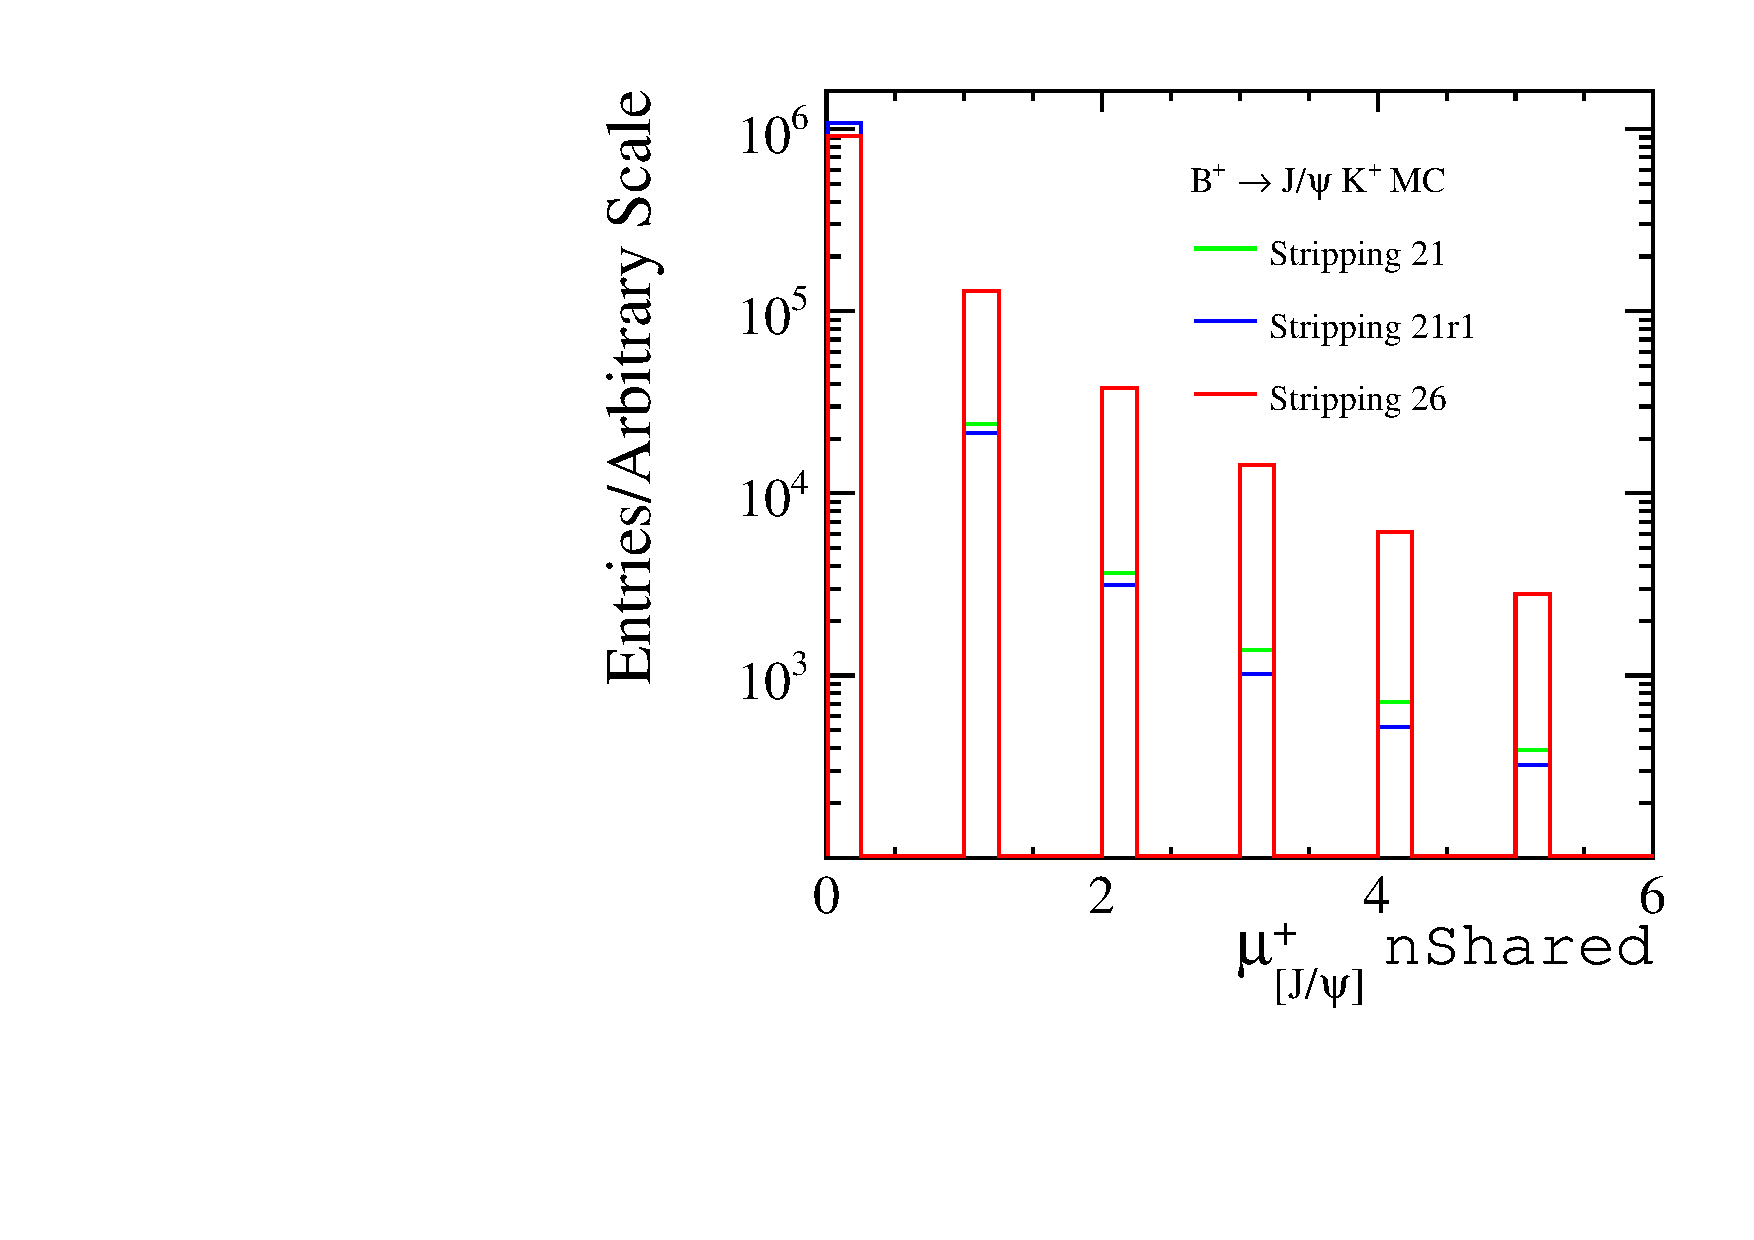
\includegraphics[width=0.5\linewidth]{trimuon/plotvariablewantlogtruemu1_nSharedJPSIKMC.pdf}\put(-40,133){(a)}
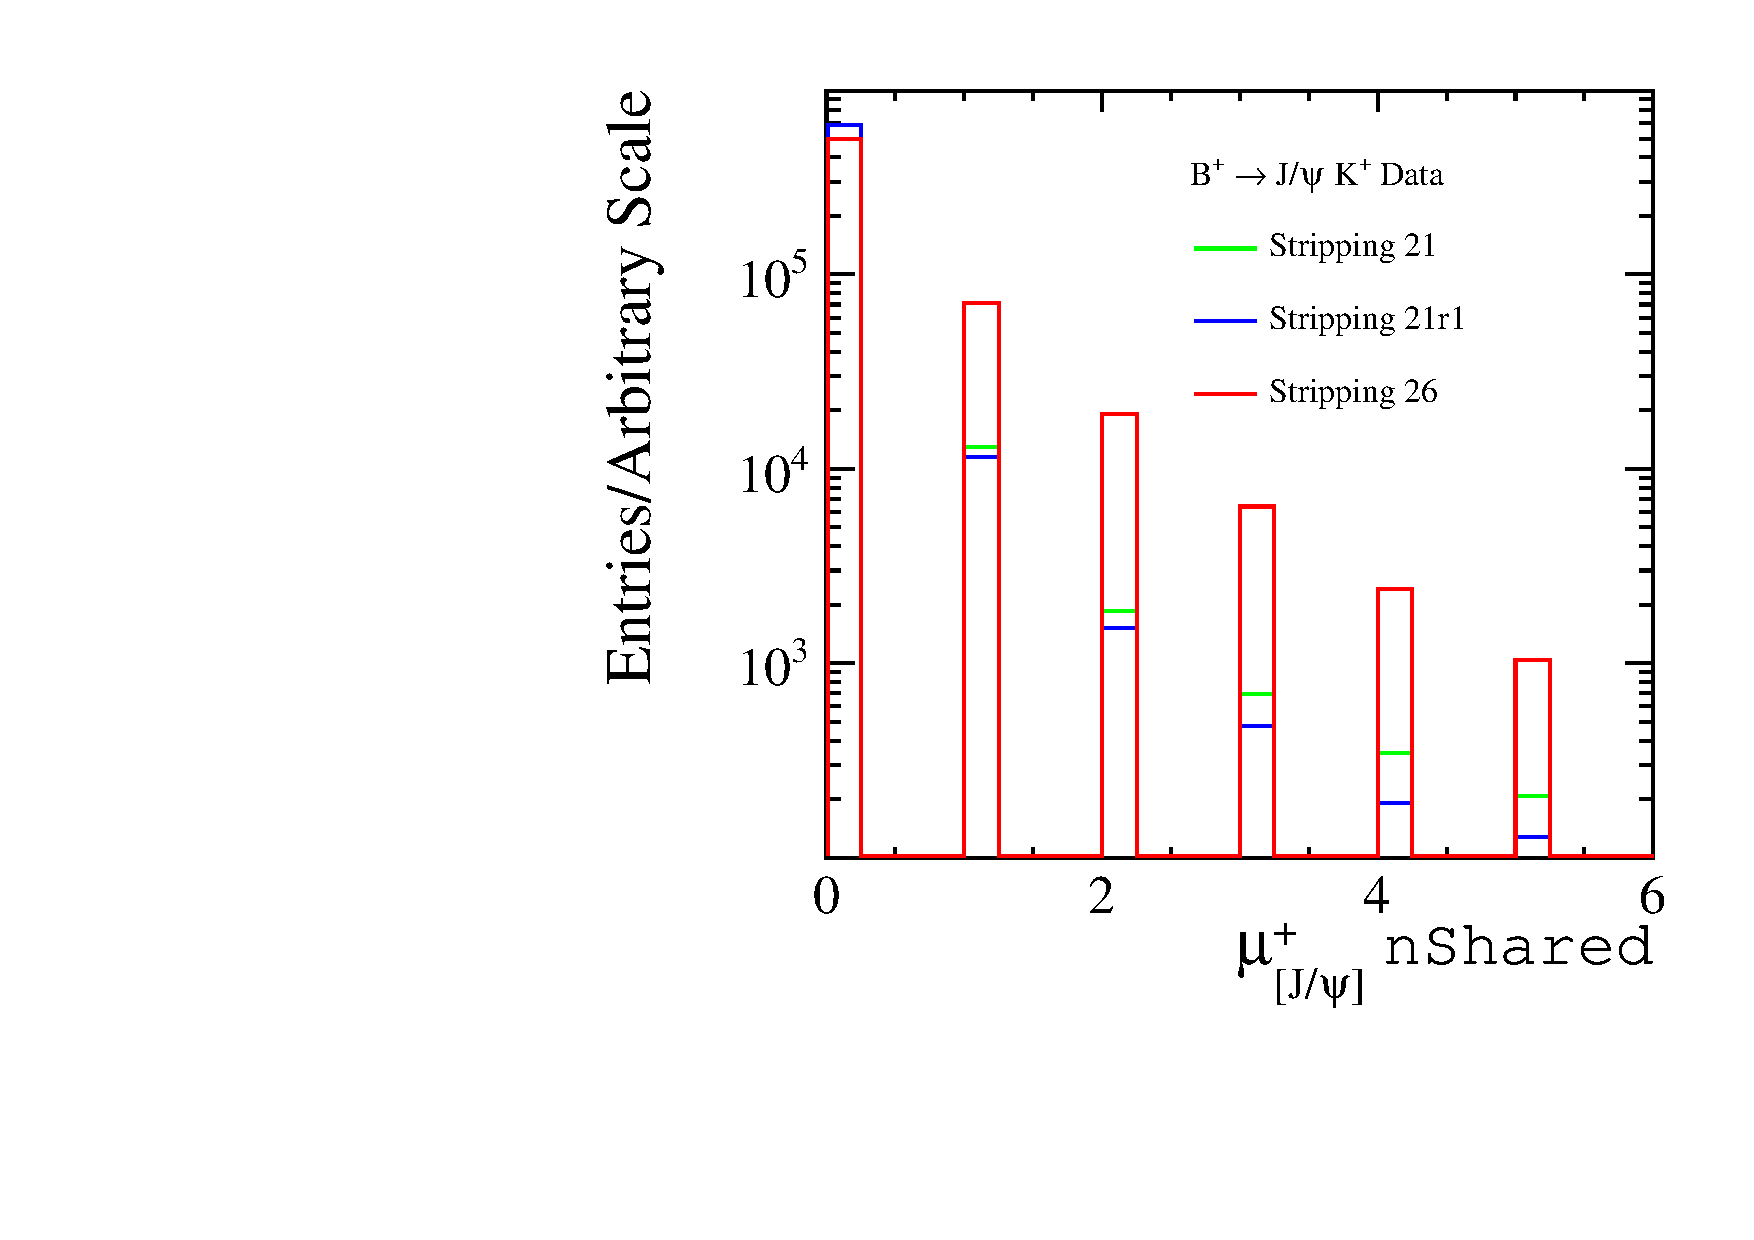
\includegraphics[width=0.5\linewidth]{trimuon/plotvariablewantlogtruemu1_nSharedJPSIKDATA.pdf}\put(-40,133){(b)}
	\caption{(a) \texttt{nShared} variable distribution for the positive muon in \bjpsimumuk decays in (a) simulation and (b) data. Different stripping versions corresponding to 2012 (\textit{Stripping 21}), 2011 (\textit{Stripping 21r1}), 2016 (\textit{Stripping 26}) data-taking are shown. The distributions are normalised to have the same area. There is shift of distribution in \textit{Stripping 26} towards less isolated tracks. The proportion of muon tracks that share no other hits with other tracks is smaller, whereas the proportion of the tracks sharing hits with other muon track is increasing.}
\label{fig:nSharedvar}
%\vspace*{-1.0cm}
\end{figure}

Using the same calibration channels as in~\autoref{muonperf}, misID and ID rates can be seen in Figure~\ref{fig:nSharedRun1andRun2}. As the tracks tend to be less isolated in \textit{Stripping 26}, typical of non-signal like events, the misID rate is expected to be higher for the same working point (ID efficiency). While the issues highlighted here can be fixed with a reprocessing of the data, this is not expected to happen before 2019 or 2020.

\begin{figure}[h!]
\centering
%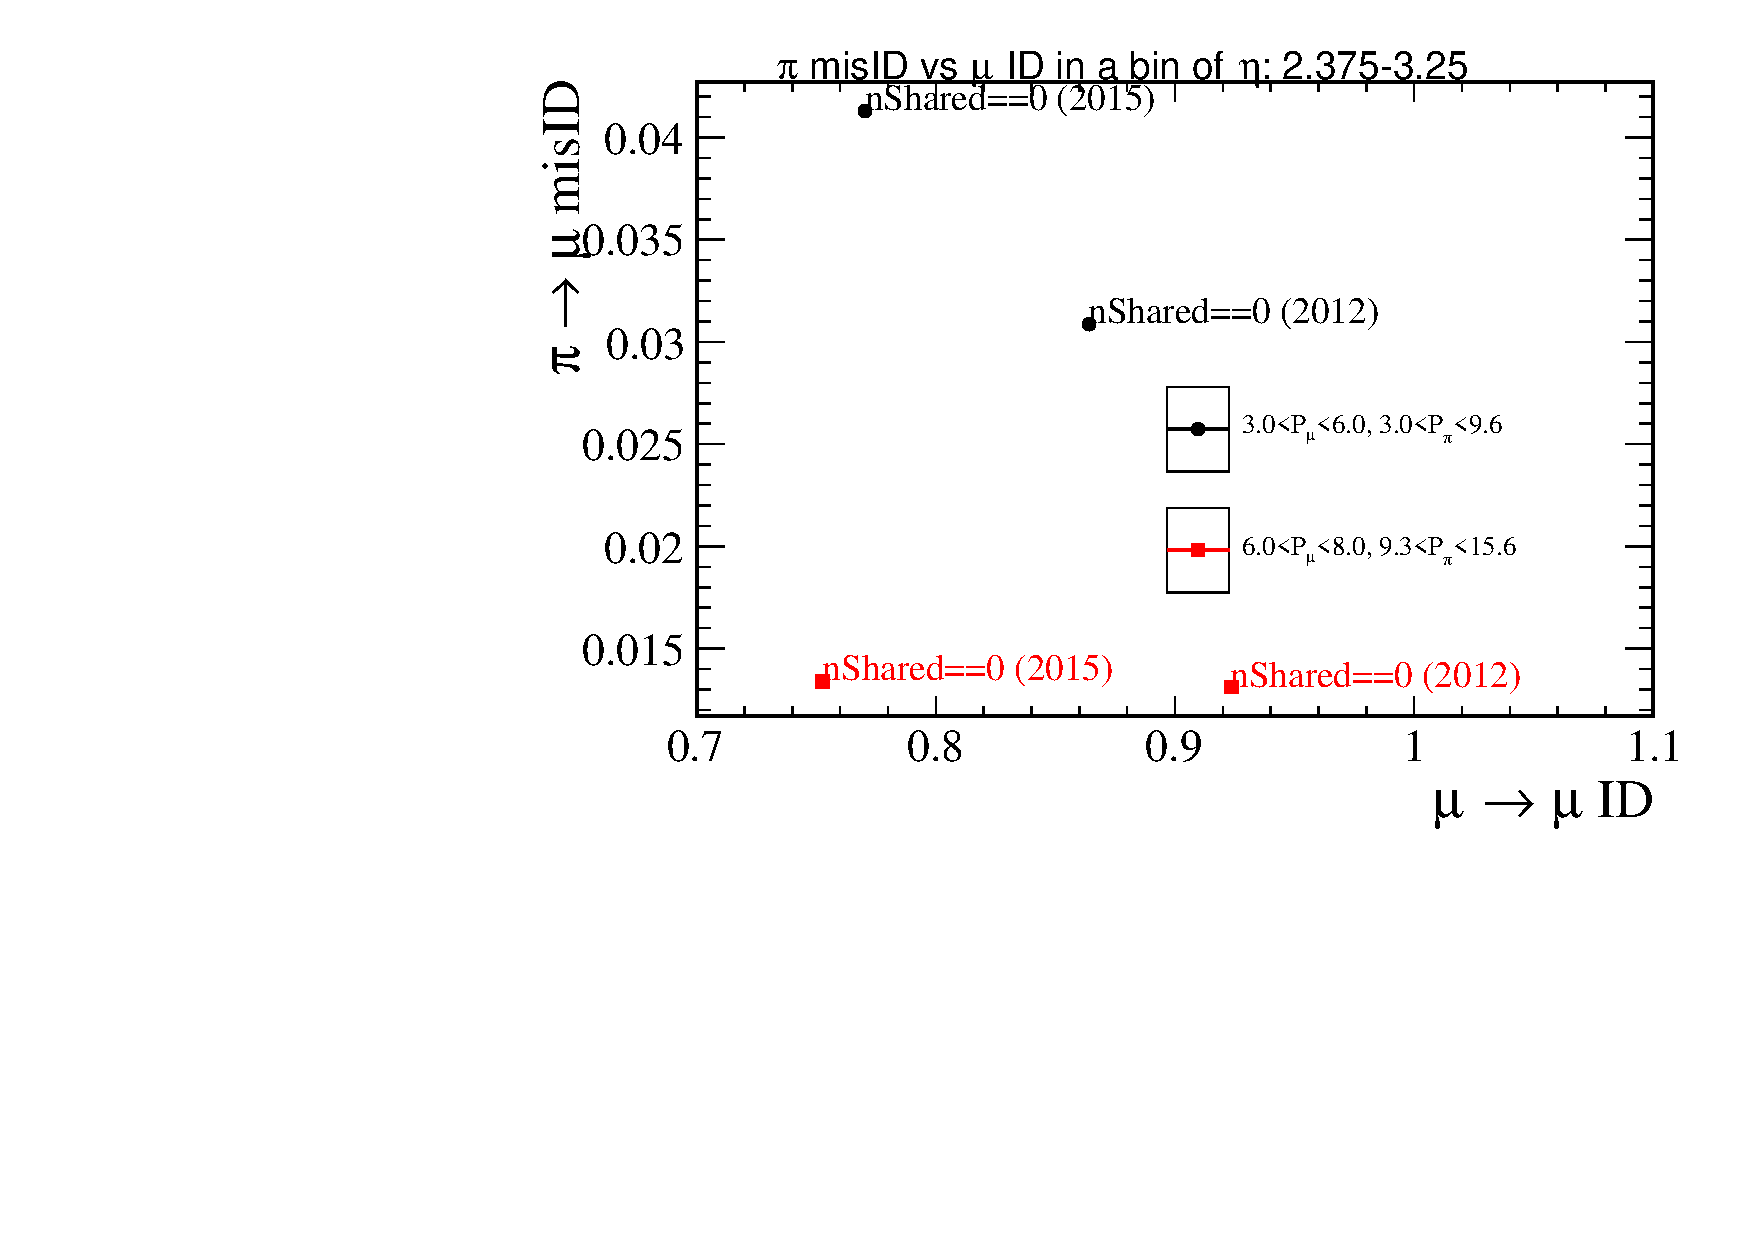
\includegraphics[width=0.52\linewidth]{compareRun1and2016selection/final_comparedirectly2012vs2015_nolog.pdf}%
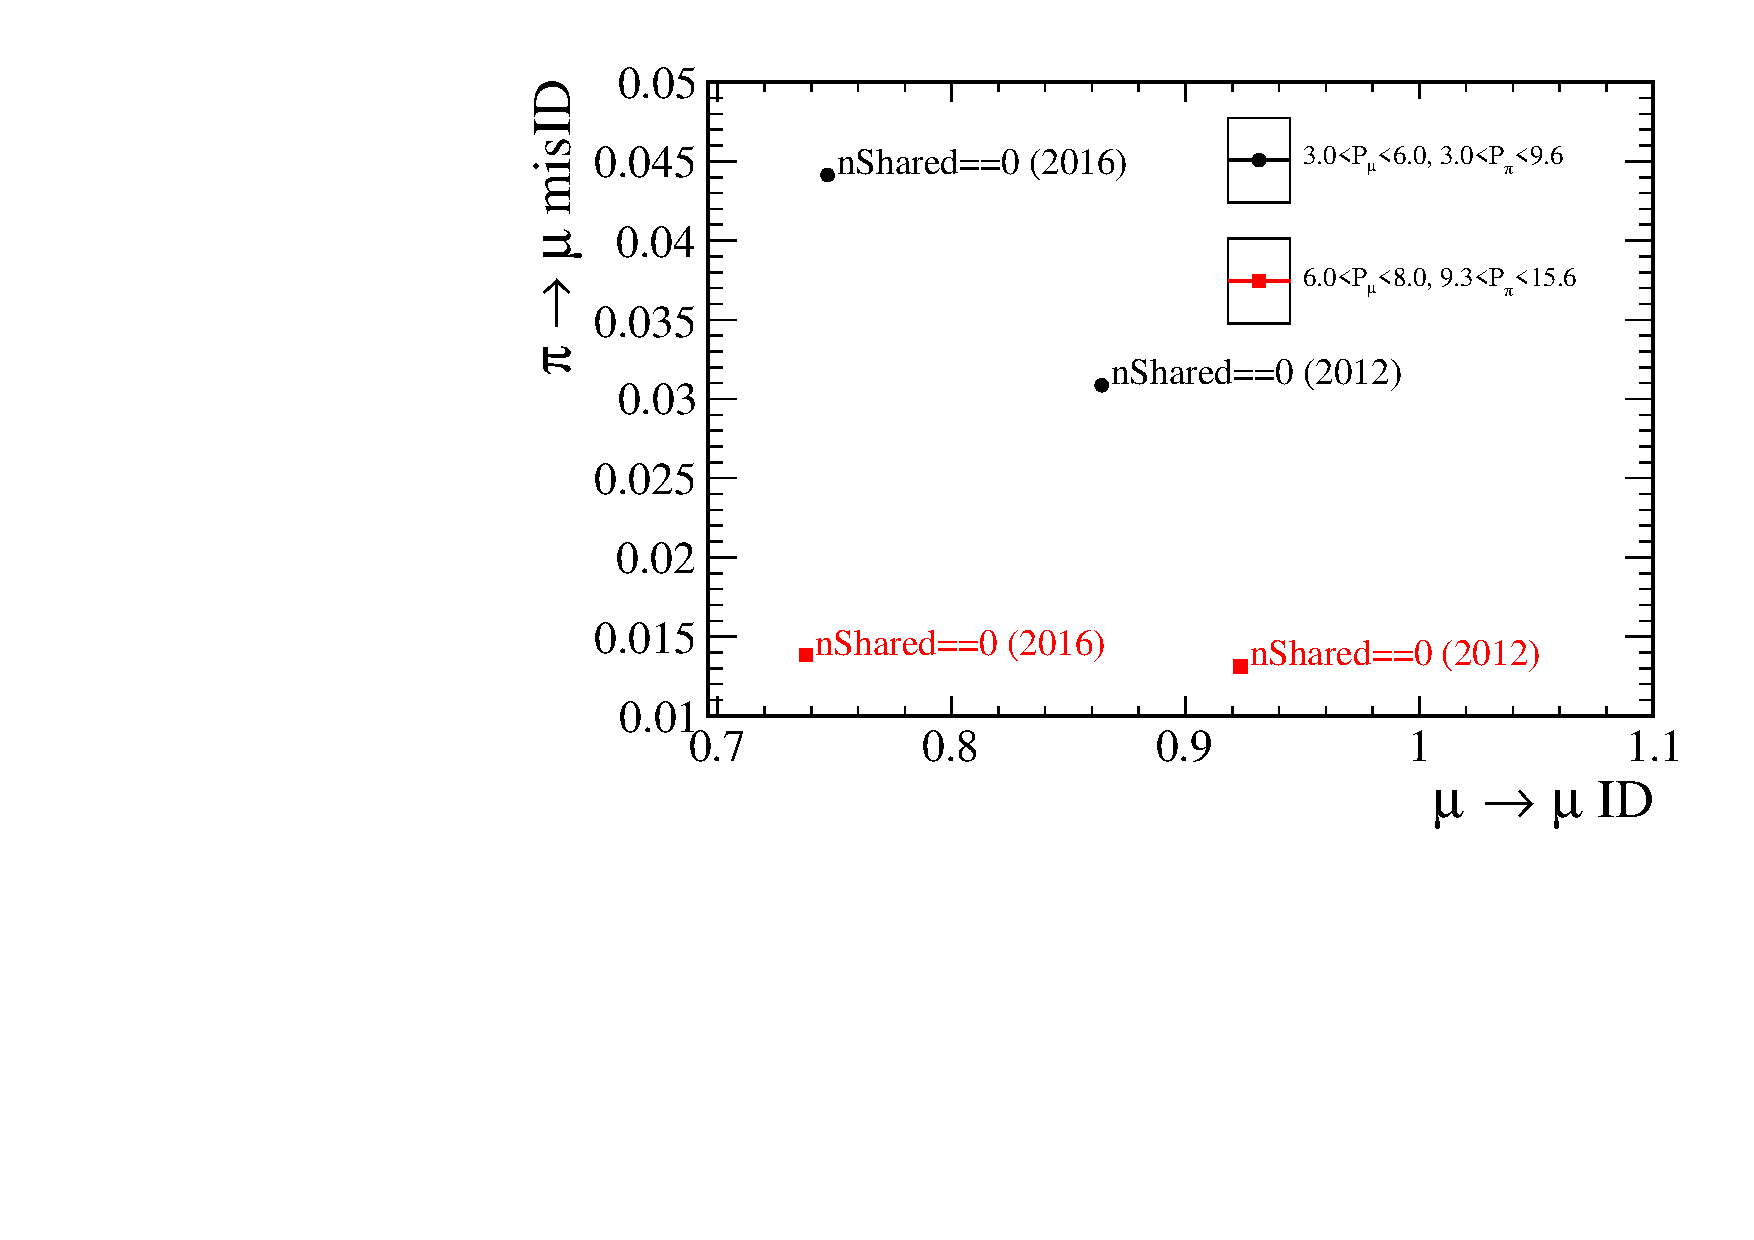
\includegraphics[width=0.7\linewidth]{trimuon/final_pretty_2016_pion.pdf}
	\caption{ID and misID probabilities from standard calibration datasets from 2012 (\textit{Stripping 21}) and 2016 (\textit{Stripping 26}), binned using the default 2-dimensional binning scheme in momentum $p$ and pseudorapidity $\eta$. In this plot, ID and misID rates in the central bin of $\eta$, 2.375<$\eta$<3.25, and the first and second bin in $p$ are compared. This demonstrates that for the same pion ID efficiency, the misID rate is significantly higher in 2016 data.}
\label{fig:nSharedRun1andRun2}
%\vspace*{-1.0cm}
\end{figure}

\subsection{Muon PID variables based on regression techniques }
\label{muonPIDprobnn}
Similar to the DLLmu variable in~\autoref{muonID}, which combines all the information from the detector into a global likelihood, it is possible to feed all the different variables to a neural network, which can then produce an output corresponding to the probability of a particle to be of a certain species. \texttt{Probnn${x}$}, where $x$ is the species of interest, is calculated and can be used also for muon identification. Compared to $\rm{DLL_{x}}$ variables, \texttt{Probnn${x}$} variables tend to have smaller correlation with the kinematics of the particle, and hence are more useful with decays where particles are soft, such as \Bmumumu. As with any machine learning algorithm, the selection of both the training sample and the input variables are important. In Run \Rn{1}, there were two tunings (trainings) introduced \texttt{V2} and \texttt{V3}, with more input variables in \texttt{V2}. Depending on the species of particles, \texttt{V2} or \texttt{V3} performed better. In the analysis of \Bmumumu, \texttt{Probnn${x}\_$V2} is used.


\section{Clones}
\label{cloniatkos}
When analysing decays with two muons of opposite charge, the \gls{LHCb} magnet bends these two muons in two opposite directions. With two muons of the same sign, the muons will instead bend in the same direction and can stay close together in both the tracking system and the muon detectors. This causes trouble for the tracking algorithm as it distinguishes these two tracks less well. It is even possible that these two same sign muon tracks are not genuine tracks, but rather subtracks or a copy of another track, \textit{clone tracks}. Two tracks are clones if they share at least 70\% of the hits in the \gls{VELO} and at least 70\% of the hits in the other T-stations. Of course, once it is established that two tracks share this percentage of hits, it has to be established which track is the clone track. This decision is based on the total number of hits and the \gls{trackchi2ndof} comparison of the two tracks.   


\begin{figure}[h!]
\centering
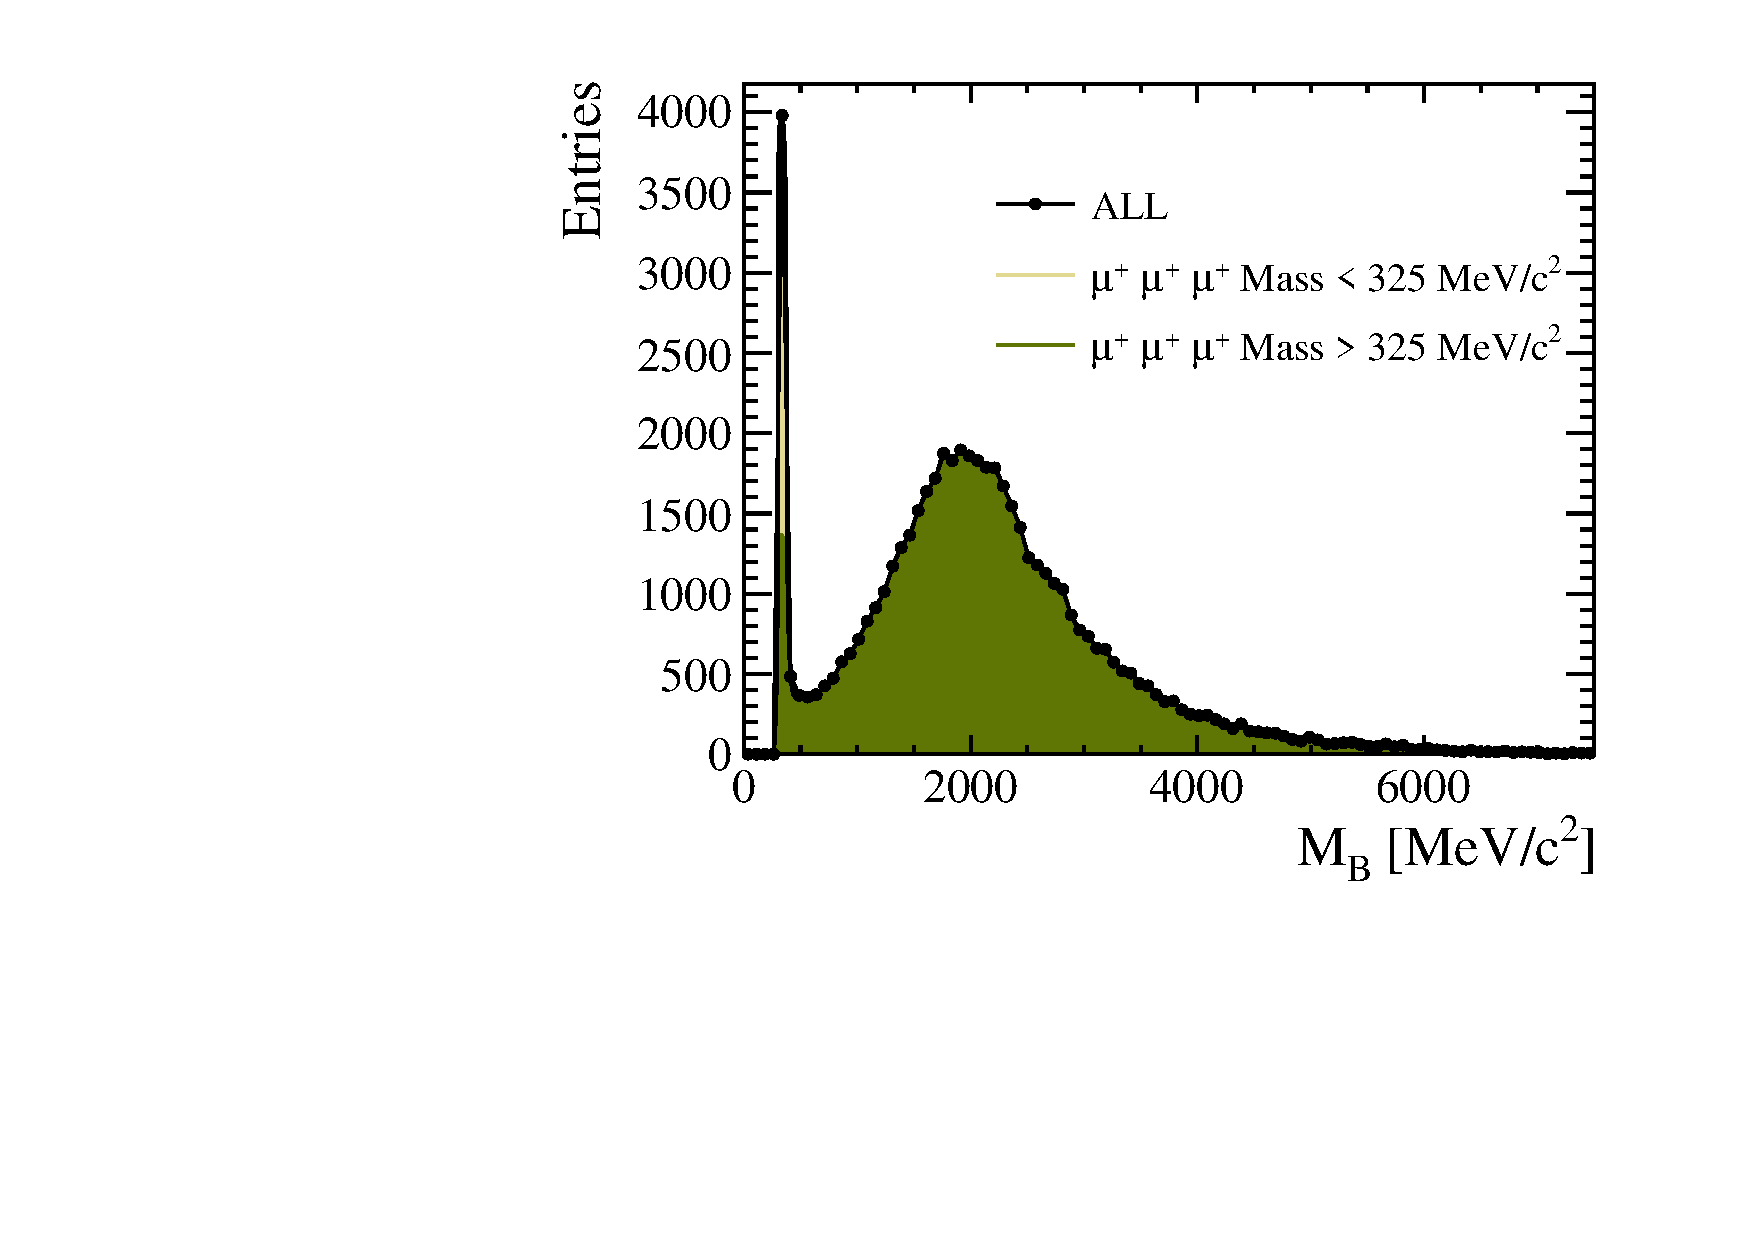
\includegraphics[width=0.5\linewidth]{trimuon/compnice_even_nicer_ONLY_STACKED_HIST_VisibleCorrM.pdf}\put(-50,133){(a)}
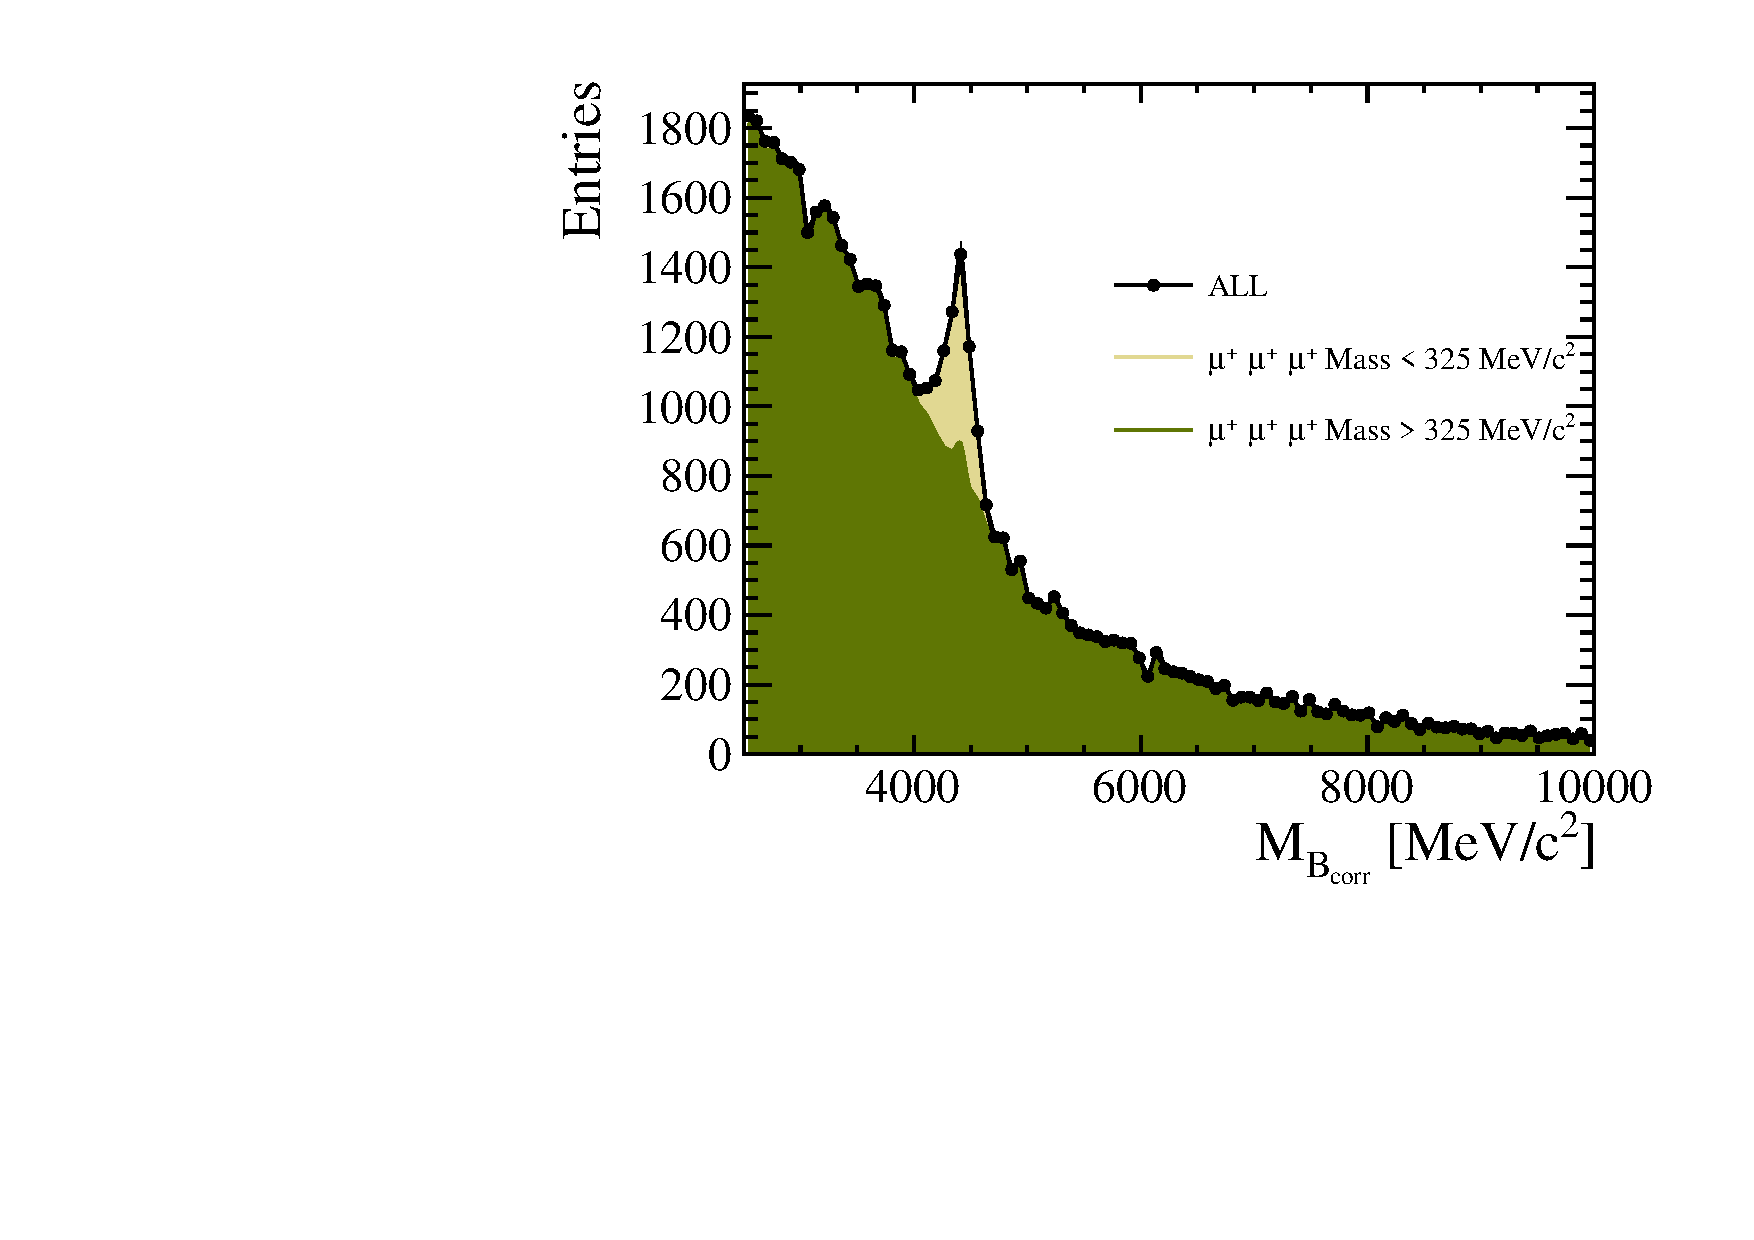
\includegraphics[width=0.5\linewidth]{trimuon/compnice_even_nicer_ONLY_STACKED_HIST_CorrM.pdf}\put(-50,133){(b)}
	\caption{(a) Visible and (b) corrected mass of \Bmumumu candidates in 2012 data where all the muons have the same charge. Clear fake peaks, arising from the correlation of several effects in the detector can be seen. }
\label{fig:Clones}
%\vspace*{-1.0cm}
\end{figure}


In search for \Bmumumu, two muons have the same charge, and hence are affected by the \textit{clones}, which needs to be understood. In a control sample from data corresponding to 2012 data-taking period, which have three muon candidates of the same charge, the effect is even more prominent and can create potentially \textit{fake peaks} in visible mass spectrum. \textit{Clones} peak at well defined visible mass 
\begin{equation}
	M_{B}=\sqrt{(3 \times M_{\mu})^{2}}\approx 318 \mevcc
	\label{eq:invmass}
\end{equation}

Once translated into corrected mass, these \textit{fake peaks} are smeared and look like genuine resonances with resolution as seen in~\autoref{fig:Clones}.  


The shape emulating a genuine resonance arises as a collective effect from vertexing, tracking and trigger selection. As there are three parallel tracks, the vertex of the system is not well defined. However, the vertex fitting of the \gls{PV} and secondary (decay) vertex (\gls{SV}) is functional and \gls{vertexchi2ndof} is good as these tracks are subtracks of each other. The distance between \gls{PV} and \gls{SV} is defined as flight distance (\gls{FD}). However, \textit{clones} can be differentiated by the position of the decay vertex of $B$,~\autoref{fig:ClonesFD} as well as the transverse position of the track in the tracking, \gls{OT} as seen in~\autoref{fig:ClonesOT}.

\begin{figure}[h!]
\centering
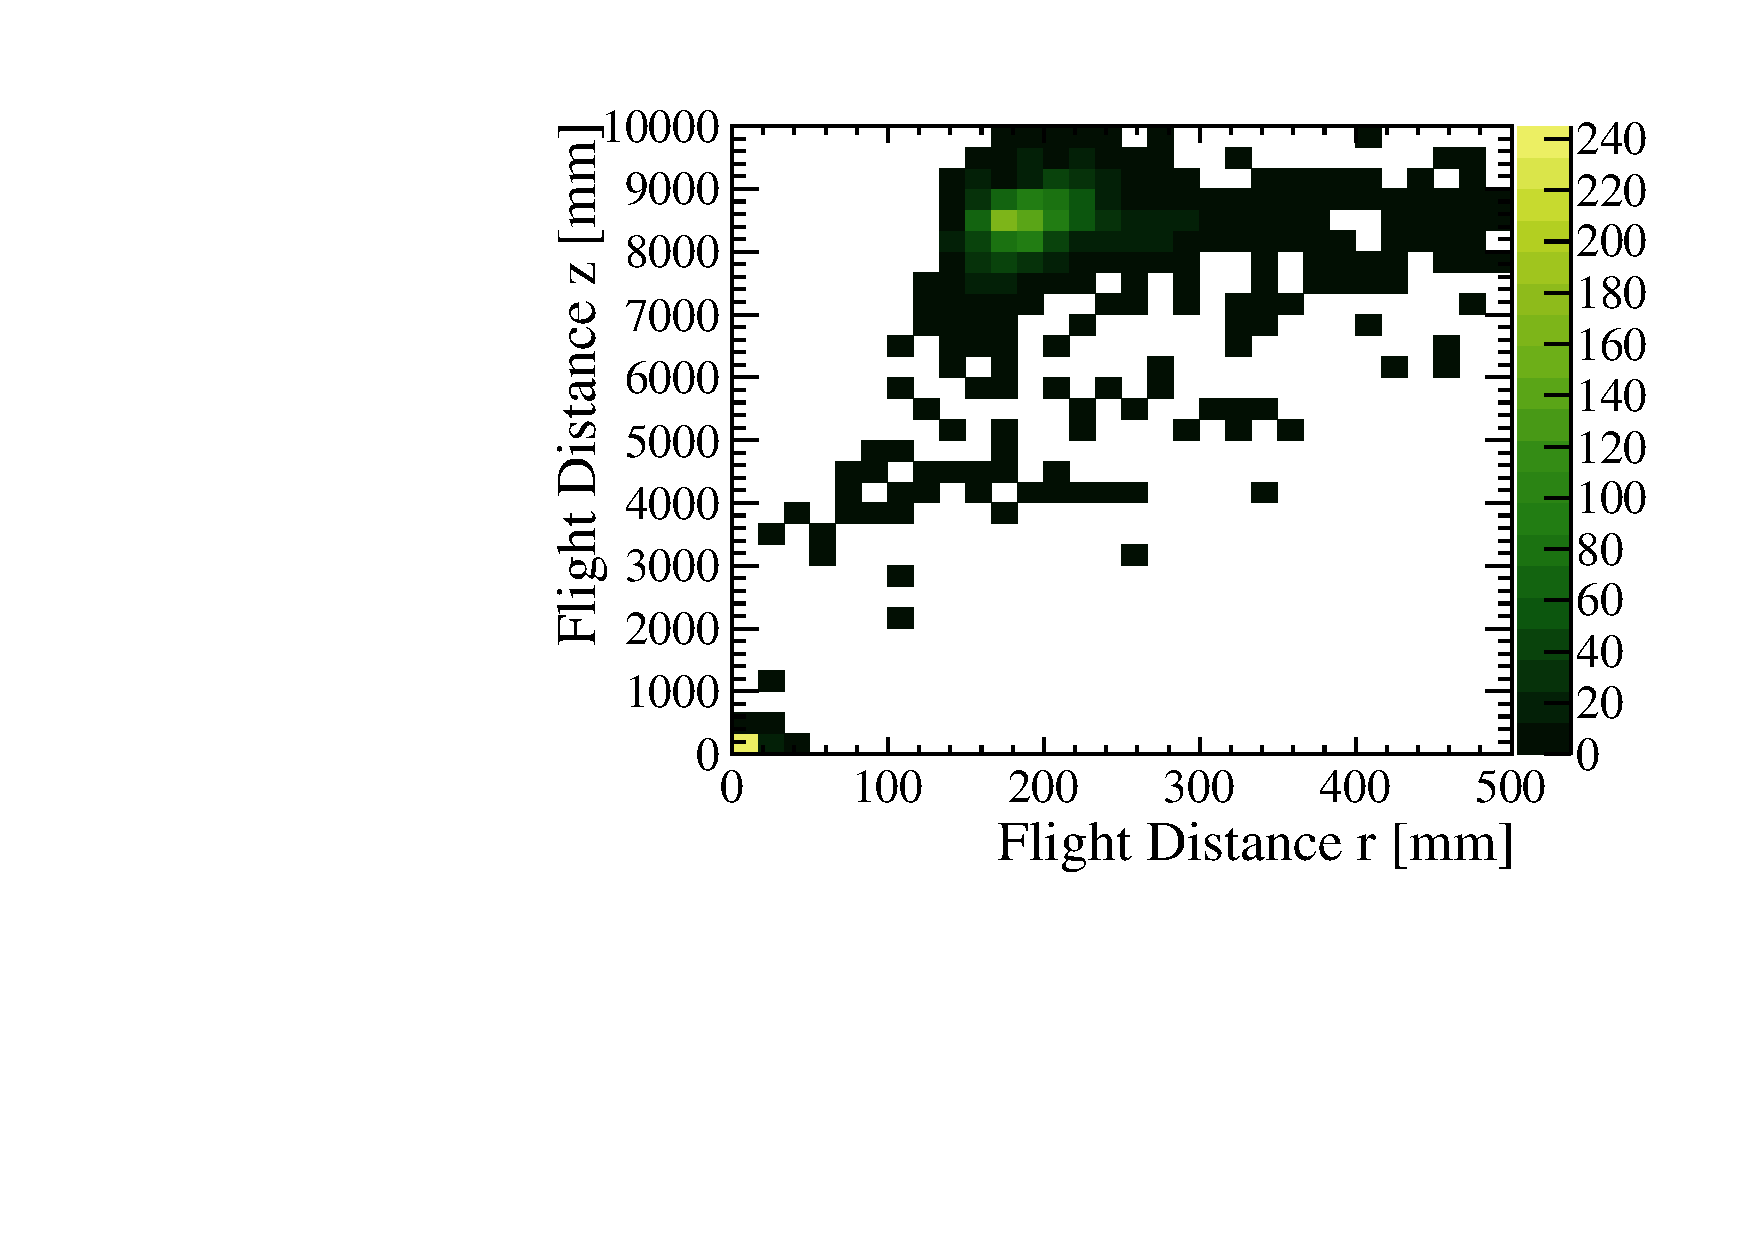
\includegraphics[width=0.5\linewidth]{trimuon/VertexInfoClone.pdf}\put(-50,133){(a)}
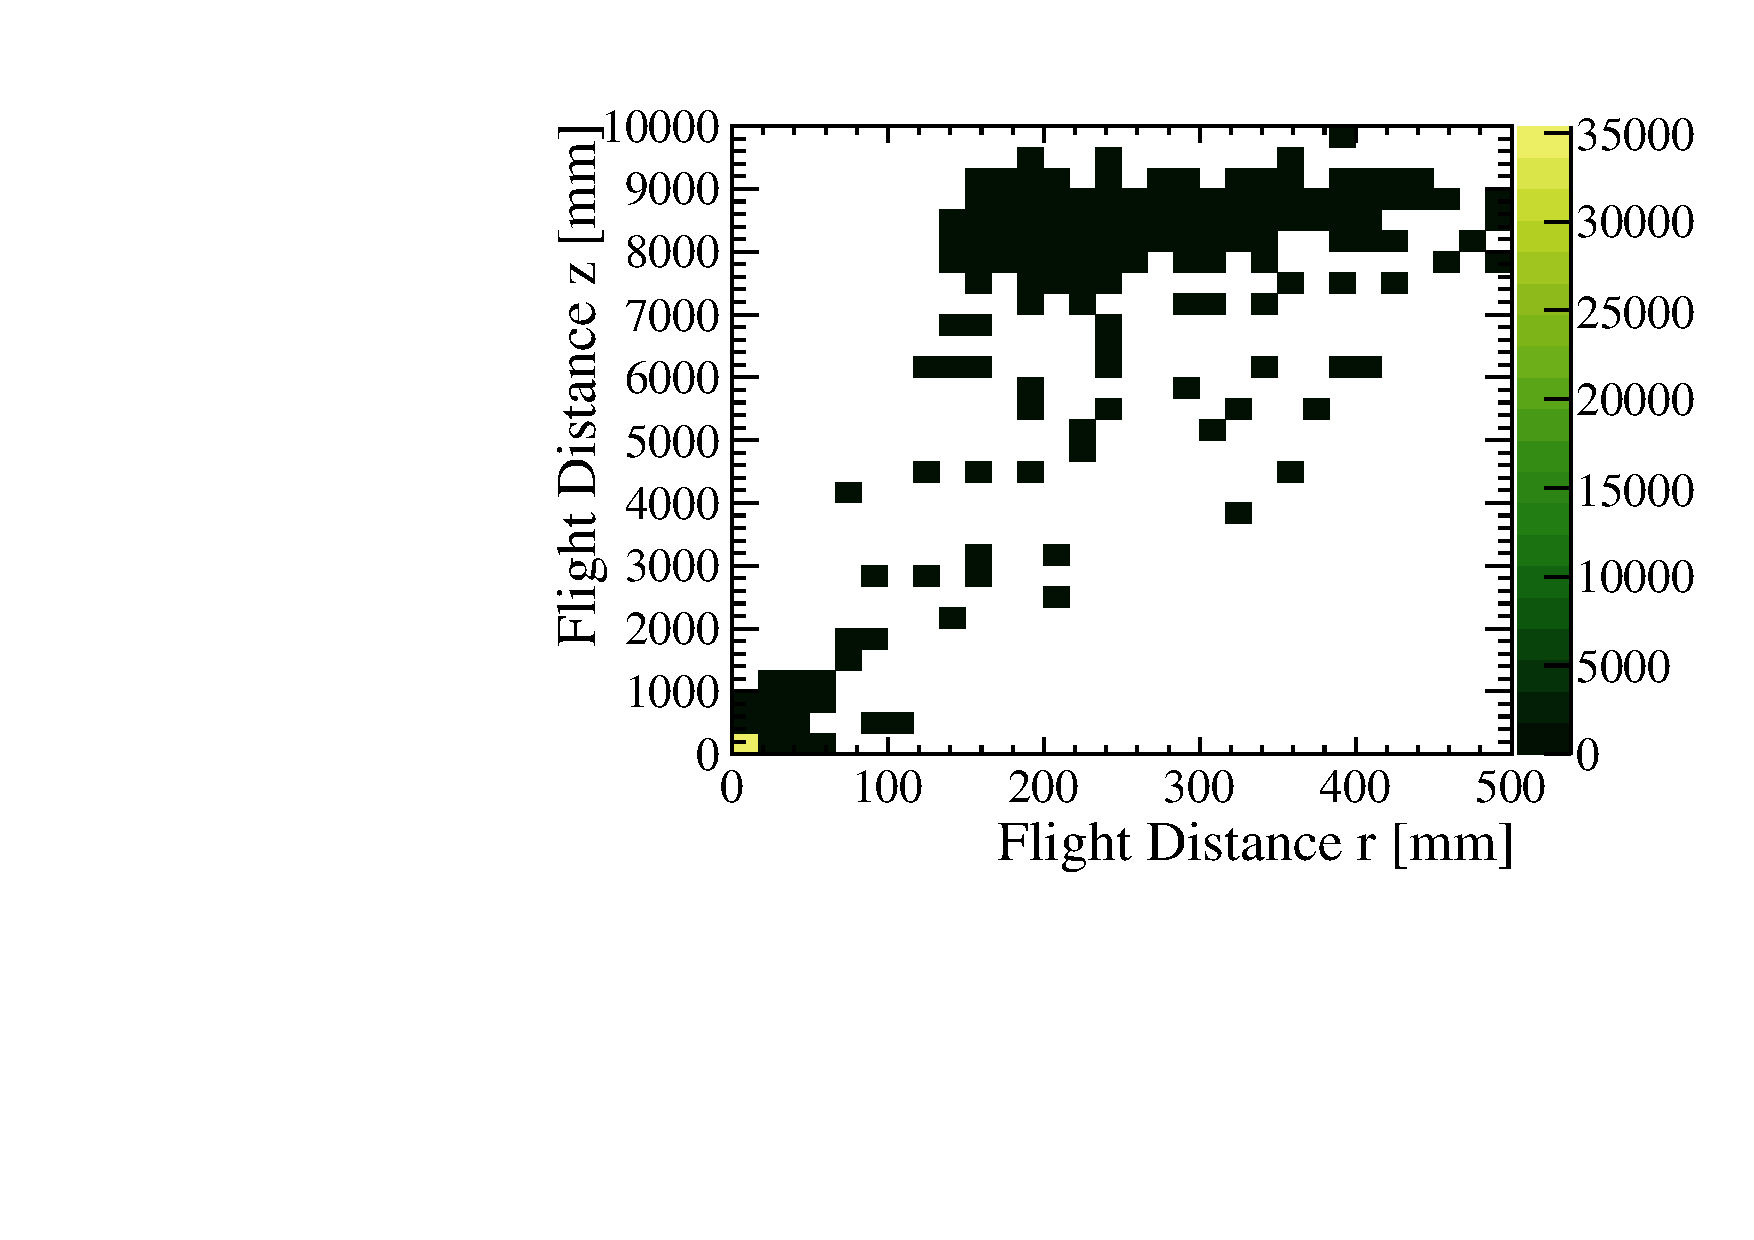
\includegraphics[width=0.5\linewidth]{trimuon/VertexInfoNoClone.pdf}\put(-50,133){(b)}
	\caption{(a) Clone and (b) no clones flight distance properties. It can be seen that \textit{clone} tracks have their decay vertex placed at the end of the detector, whereas regular good tracks will decay within the \gls{VELO}.}
\label{fig:ClonesFD}
%\vspace*{-1.0cm}
\end{figure}


\begin{figure}[h!]
\centering
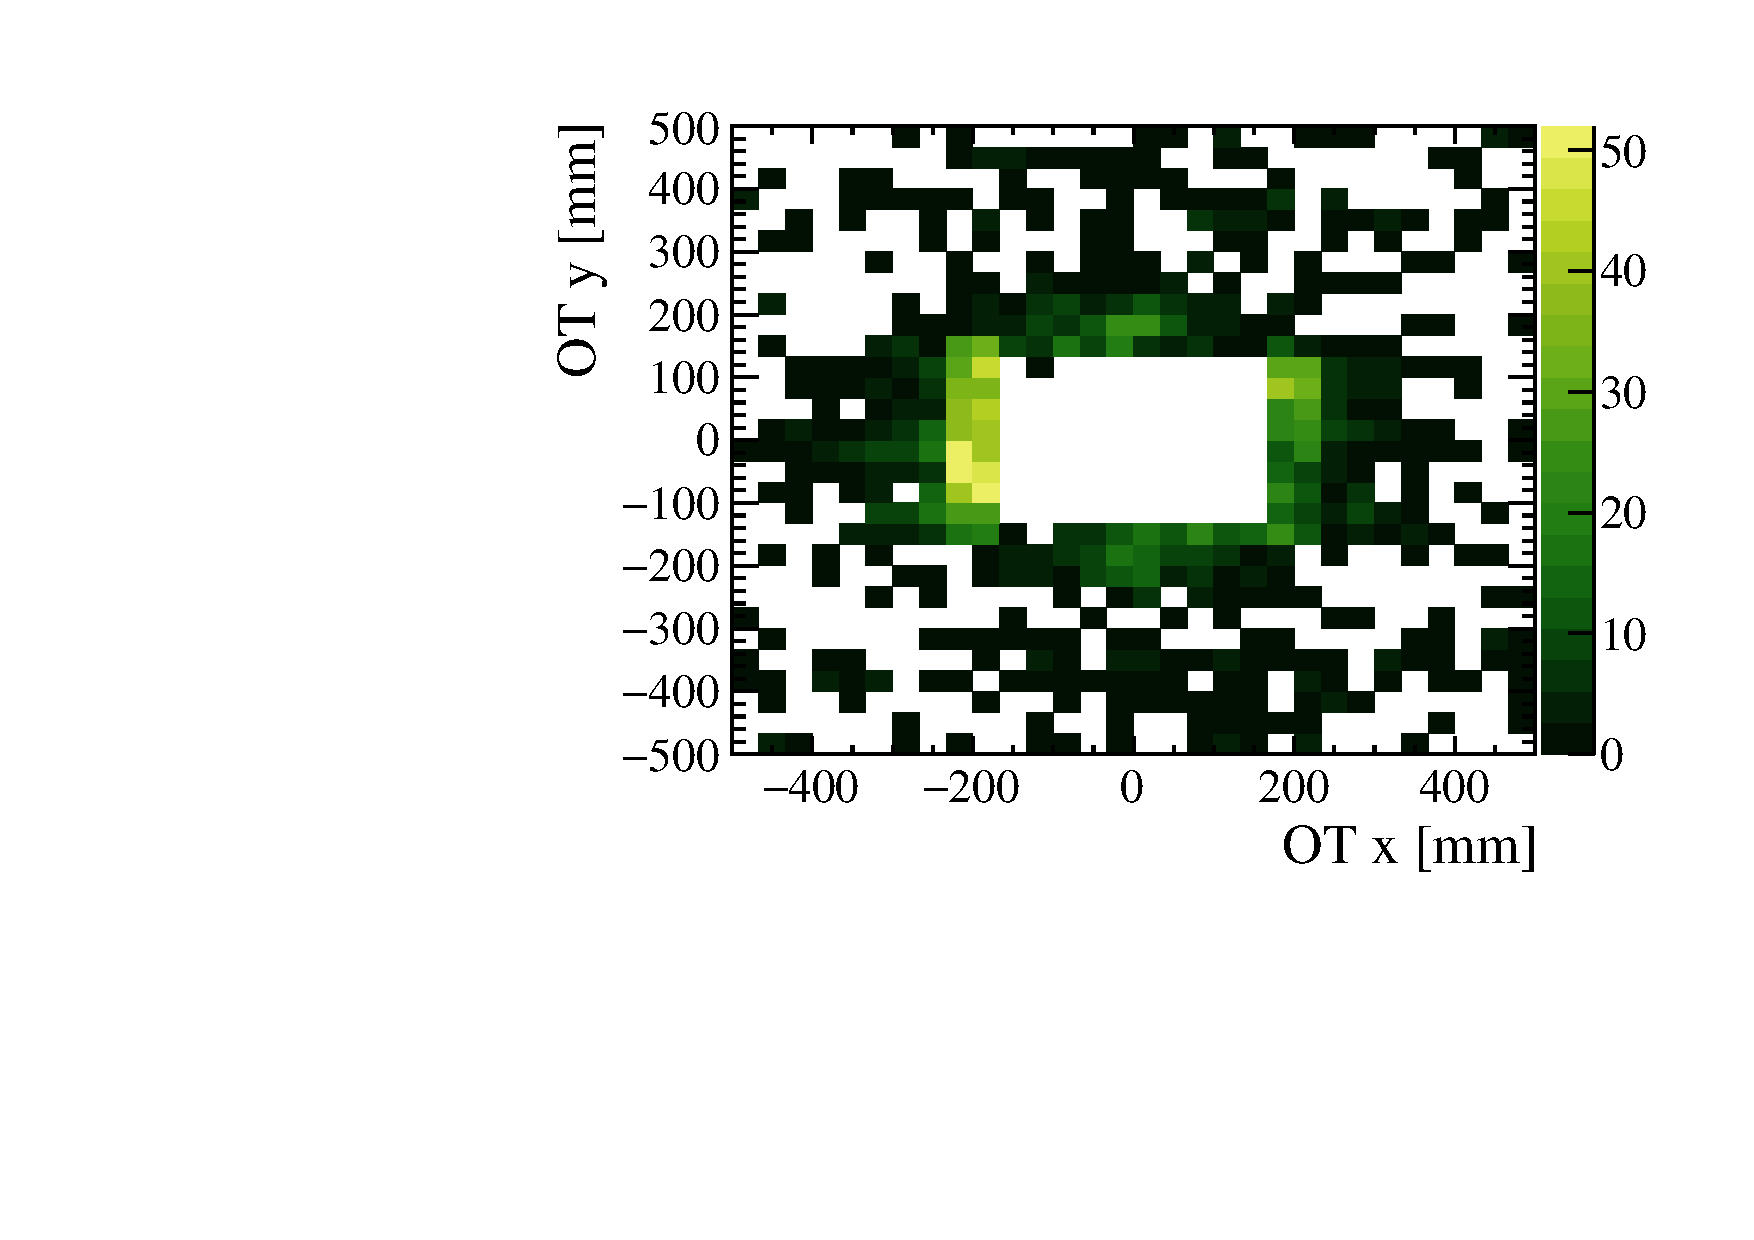
\includegraphics[width=0.5\linewidth]{trimuon/OTxandyClone.pdf}\put(-50,133){(a)}
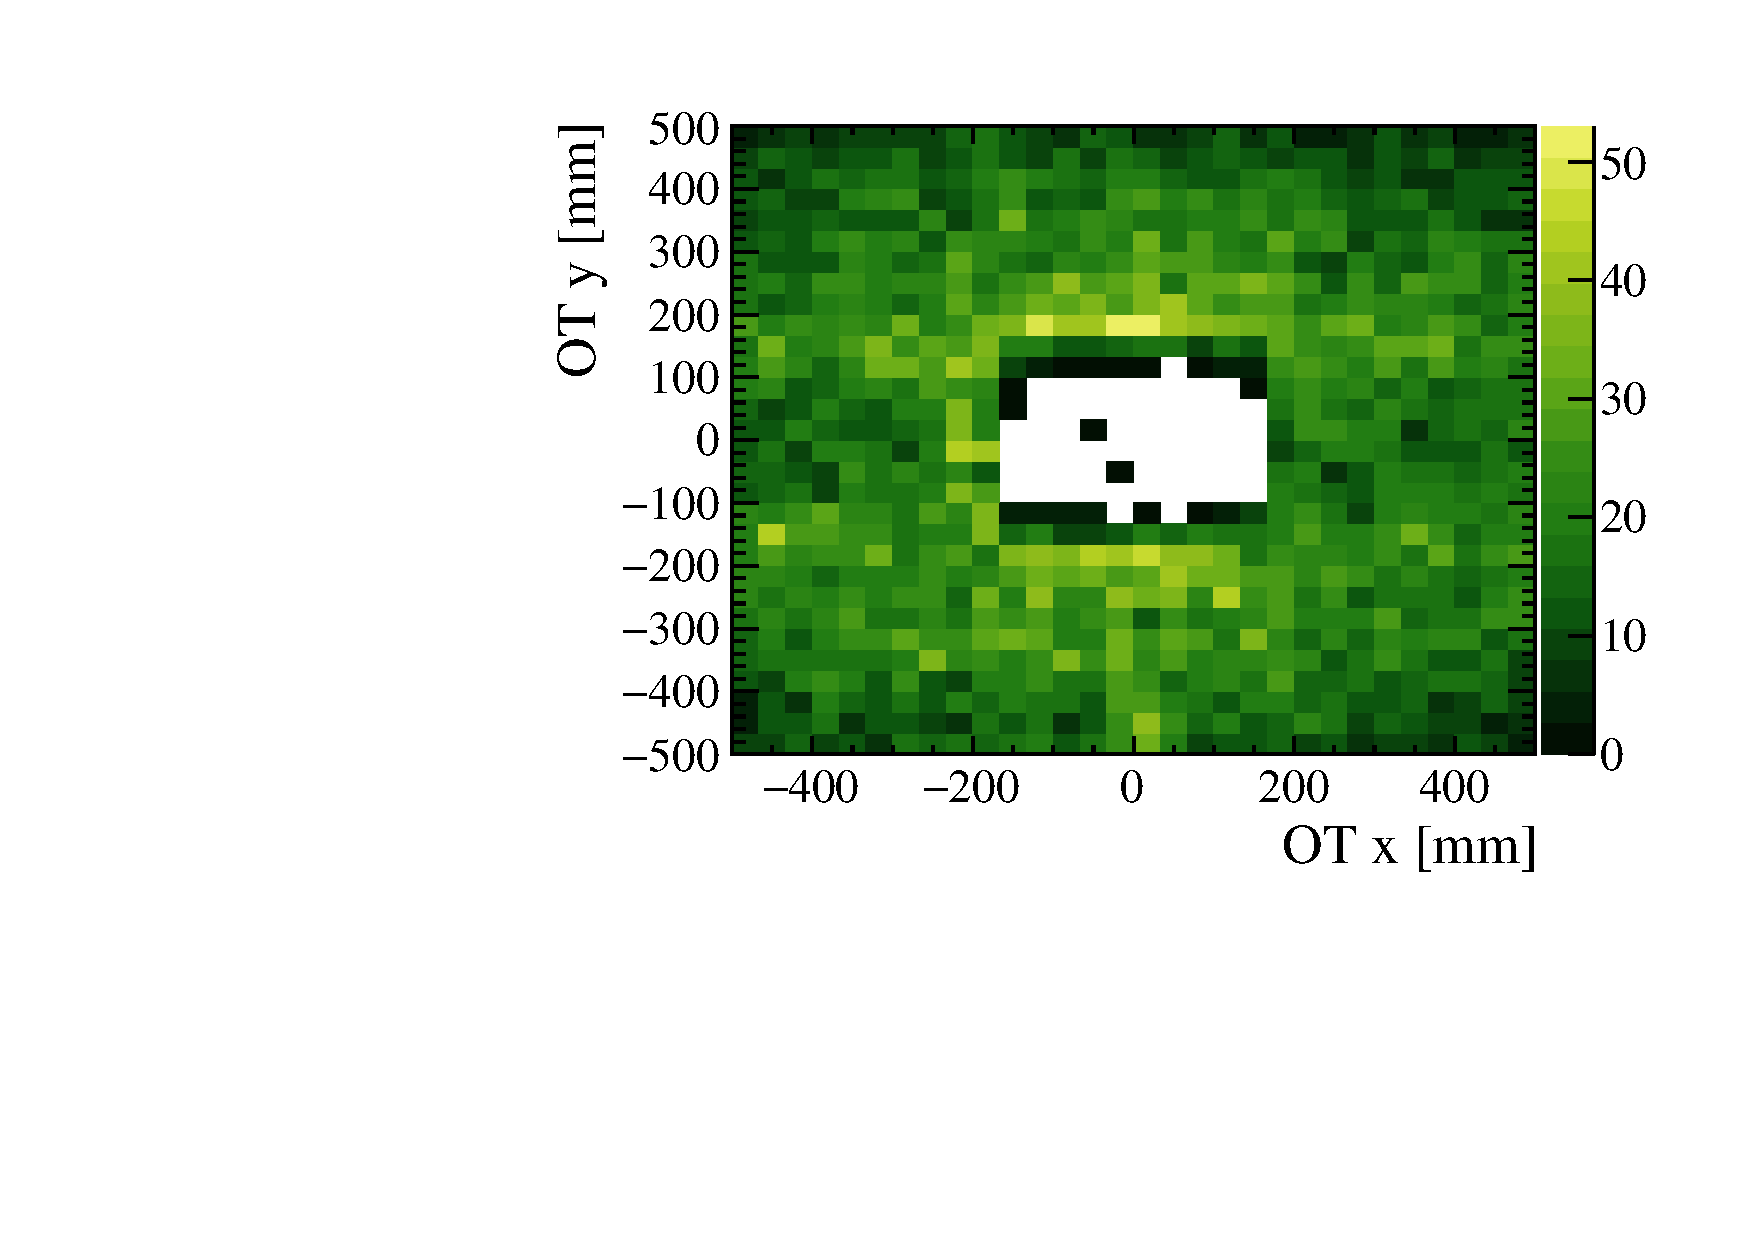
\includegraphics[width=0.5\linewidth]{trimuon/OTxandyNoClone.pdf}\put(-50,133){(b)}
	\caption{The difference in the \gls{OT} detector between (a) clones and (b) real tracks in the \Gls{OT} at the distance 9450 \mm along the \gls{LHCb}. \textit{Clones} are concentrated along the inner edge of the \gls{OT}. Good muon tracks will cover most of \gls{OT} evenly.}
\label{fig:ClonesOT}
%\vspace*{-1.0cm}
\end{figure}

With this typical path for the clones there is a fixed angle of the clones trough the detector (the angle between the muon momentum and the z-axis), which is calculated using information from \gls{OT} as

\begin{equation}
	\arctan(\theta)=\arctan\Big(\frac{\gls{FD}\ radius}{\gls{FD}\ distance\ along\ z}\Big)=\arctan\Big(\frac{200\ \mm\ (\autoref{fig:ClonesOT})}{8500\ \mm}\Big) = 0.023 \rm{rad}. 
\end{equation}


With the \texttt{L0Muon} $p_{T}$ threshold of 1.76 \gevc for 2012 \cite{Albrecht:2013fba}, the typical momentum from about 75  to 120 \gevc is yielded because

\begin{equation}
	p=1.76\gevc/\sin\bigg(\arctan\Big(\frac{200\ \mm}{8500\ \mm}\Big)\bigg).
\end{equation}

The angle between $B$ flight and trimuon momentum vector, \gls{DIRA}, will also be fixed and have typical value of 0.7 \mrad as seen in~\autoref{fig:ClonesDIRA}.

\begin{figure}[h!]
\centering
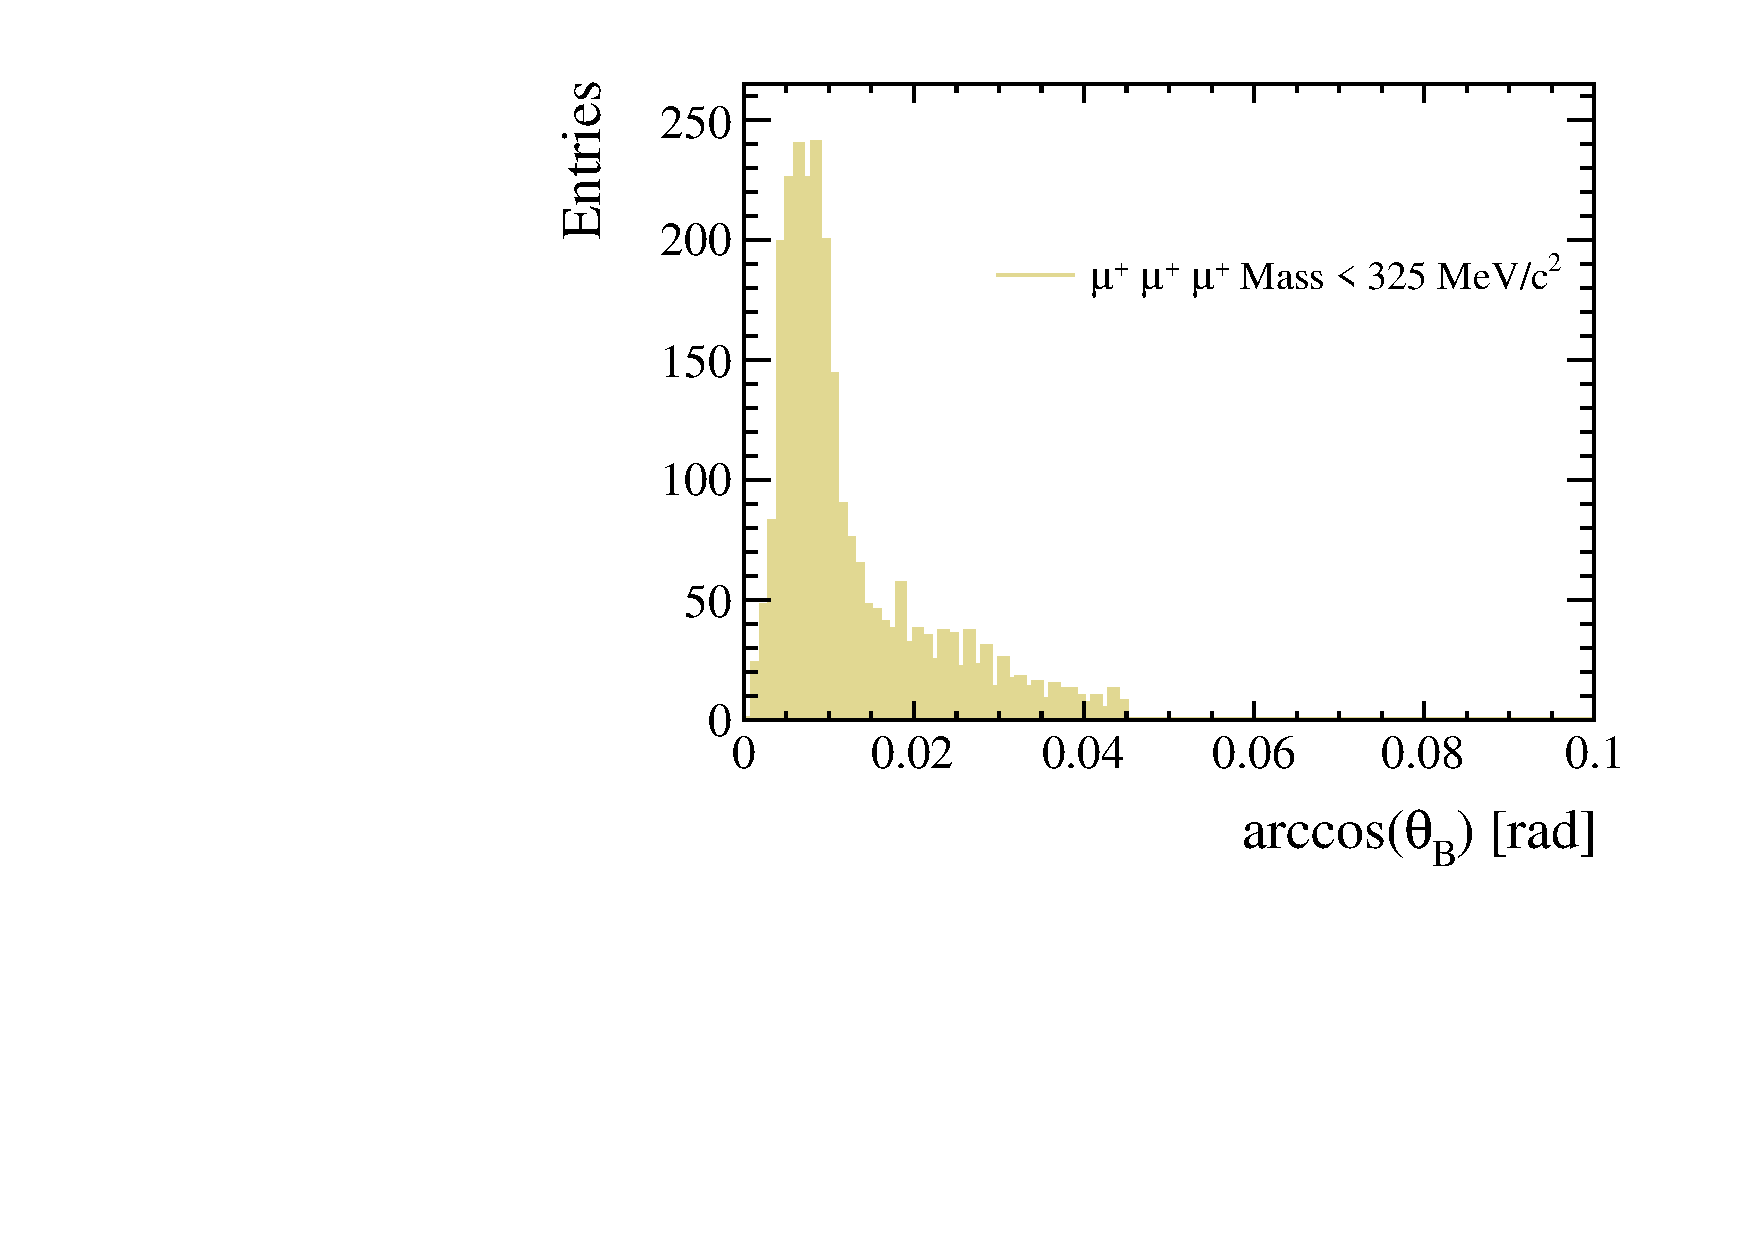
\includegraphics[width=0.5\linewidth]{trimuon/compnice_even_nicer_ONLY_STACKED_HIST_oneFILE_BplusDiraclone.pdf}\put(-50,133){(a)}
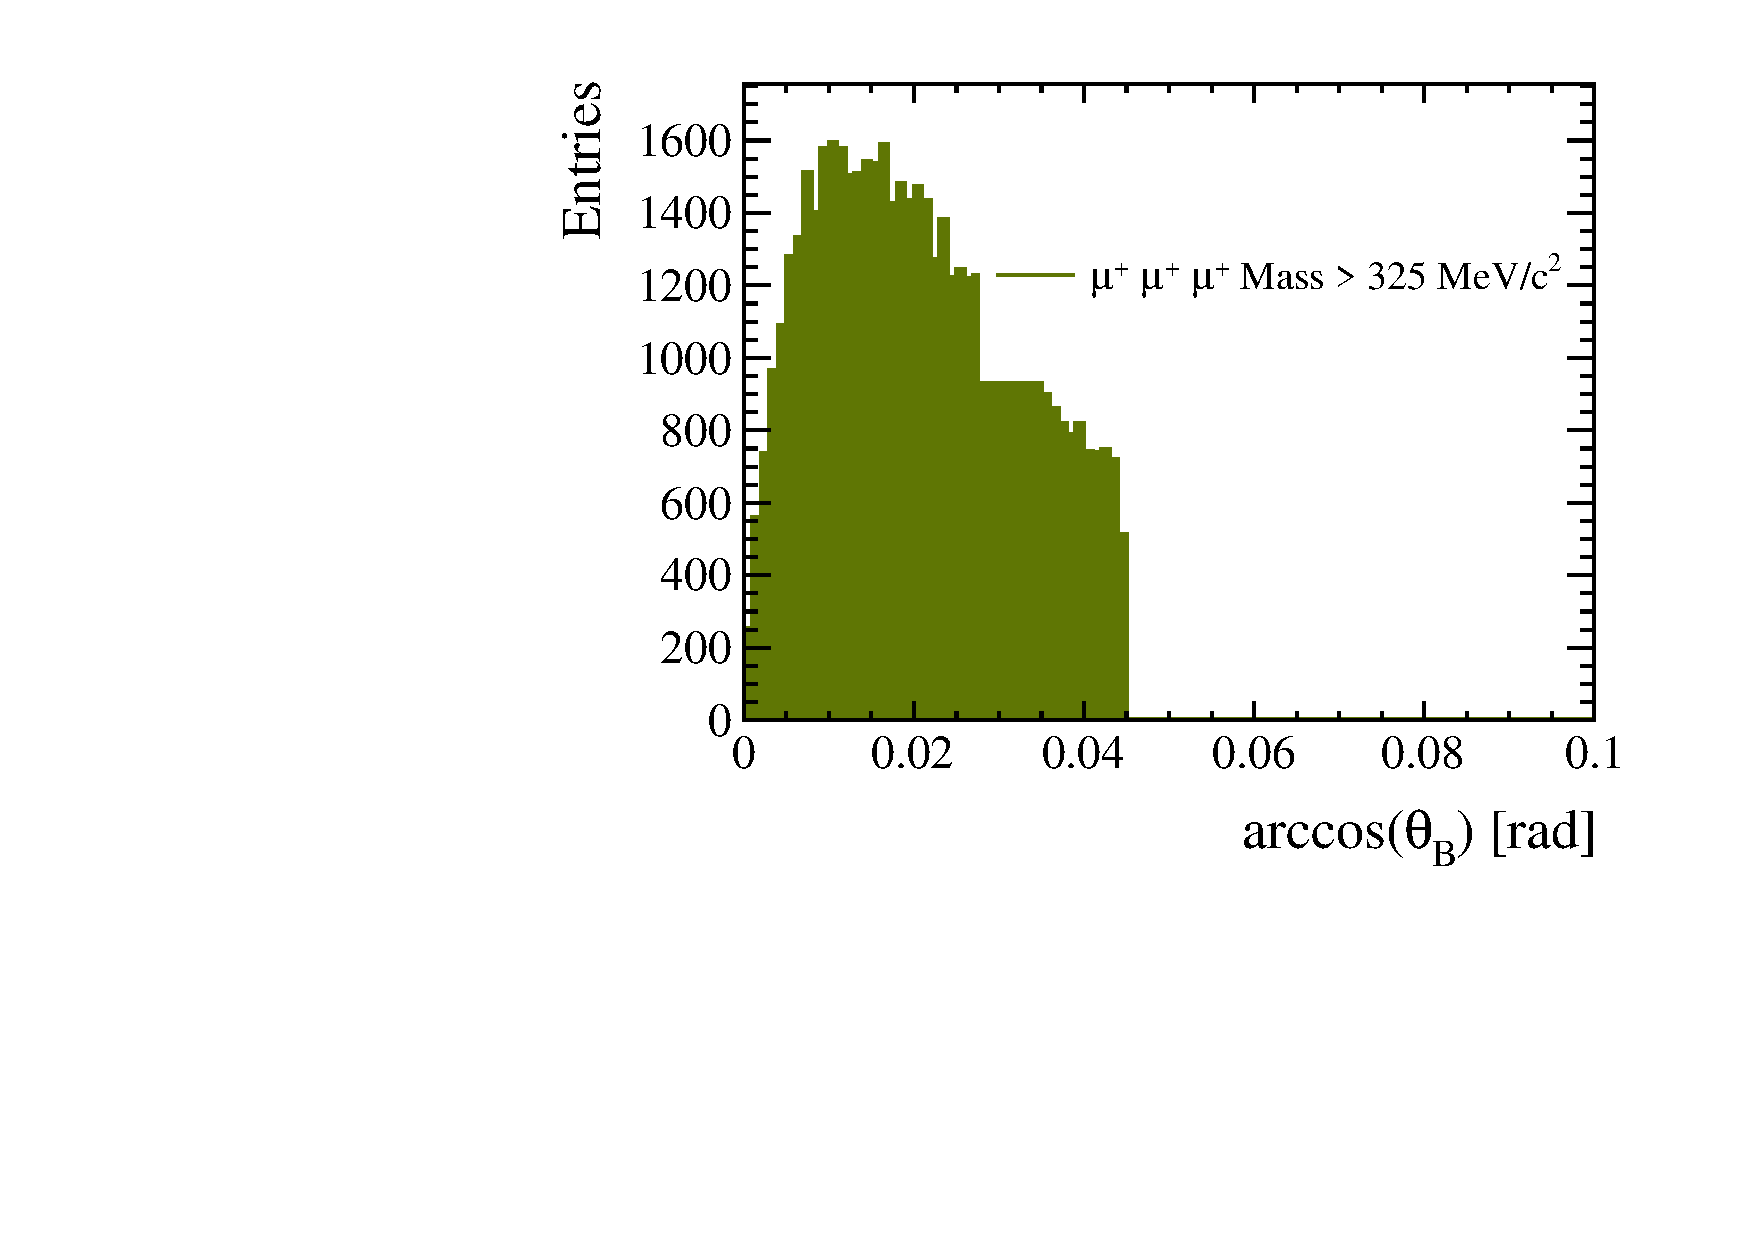
\includegraphics[width=0.5\linewidth]{trimuon/compnice_even_nicer_ONLY_STACKED_HIST_oneFILE_BplusDiranoclone.pdf}\put(-50,133){(b)}
	\caption{(a) Peaking clone distribution is visible as all of \textit{clone} tracks are collinear compared to (b) smooth no clone distribution for \gls{DIRA}.}
\label{fig:ClonesDIRA}
%\vspace*{-1.0cm}
\end{figure}

Hence, missing $p_{T}$ in the direction of the flight can be calculated using \gls{DIRA} and typical $p$,

\begin{equation}
	p_{T}=100\gevc \times \sin(0.0007)=0.7\gevc,
	\label{eq:mispt}
\end{equation}
corrected mass $M_{corr} = \sqrt{{M}^{2} + |p^{2}_{T}|} + |p_{T}| = 4.2 \gevcc$, using missing $p_{T}$ from~\autoref{eq:mispt} and visible mass of \textit{clones} from~\autoref{eq:invmass}.


In order to suppress these tracks in analysing \Bmumumu, where two muons have the same sign, any distinguishing features mentioned could be used. But the most powerful \gls{PID}-wise is requiring \texttt{nShared=0} in Run \Rn{1}, as this requirement removes all of the clones, as seen in~\autoref{fig:ClonesnShared}. 
For Run \Rn{2}, due to the introduced bugs, such strong requirement would harm signal efficiency too much so combination of \texttt{nShared<2} and \texttt{isMuonTight=1} is applied.
%\textit{this should remove them as well as nShared is increased for the non-owner track only- i assume that owner track will be that of nshared=0. I.e below nShared==3 for the clones, so for two muons nShared==2 so if there are two tracks, is ok}
\color{black}
%\newline In order to keep the signal efficiency high in 2016 data, as shown in Table ~\ref{tab:Reason}, softer condition ,$\texttt{nShared}<2$, is applied.

\begin{figure}[h!]
\centering
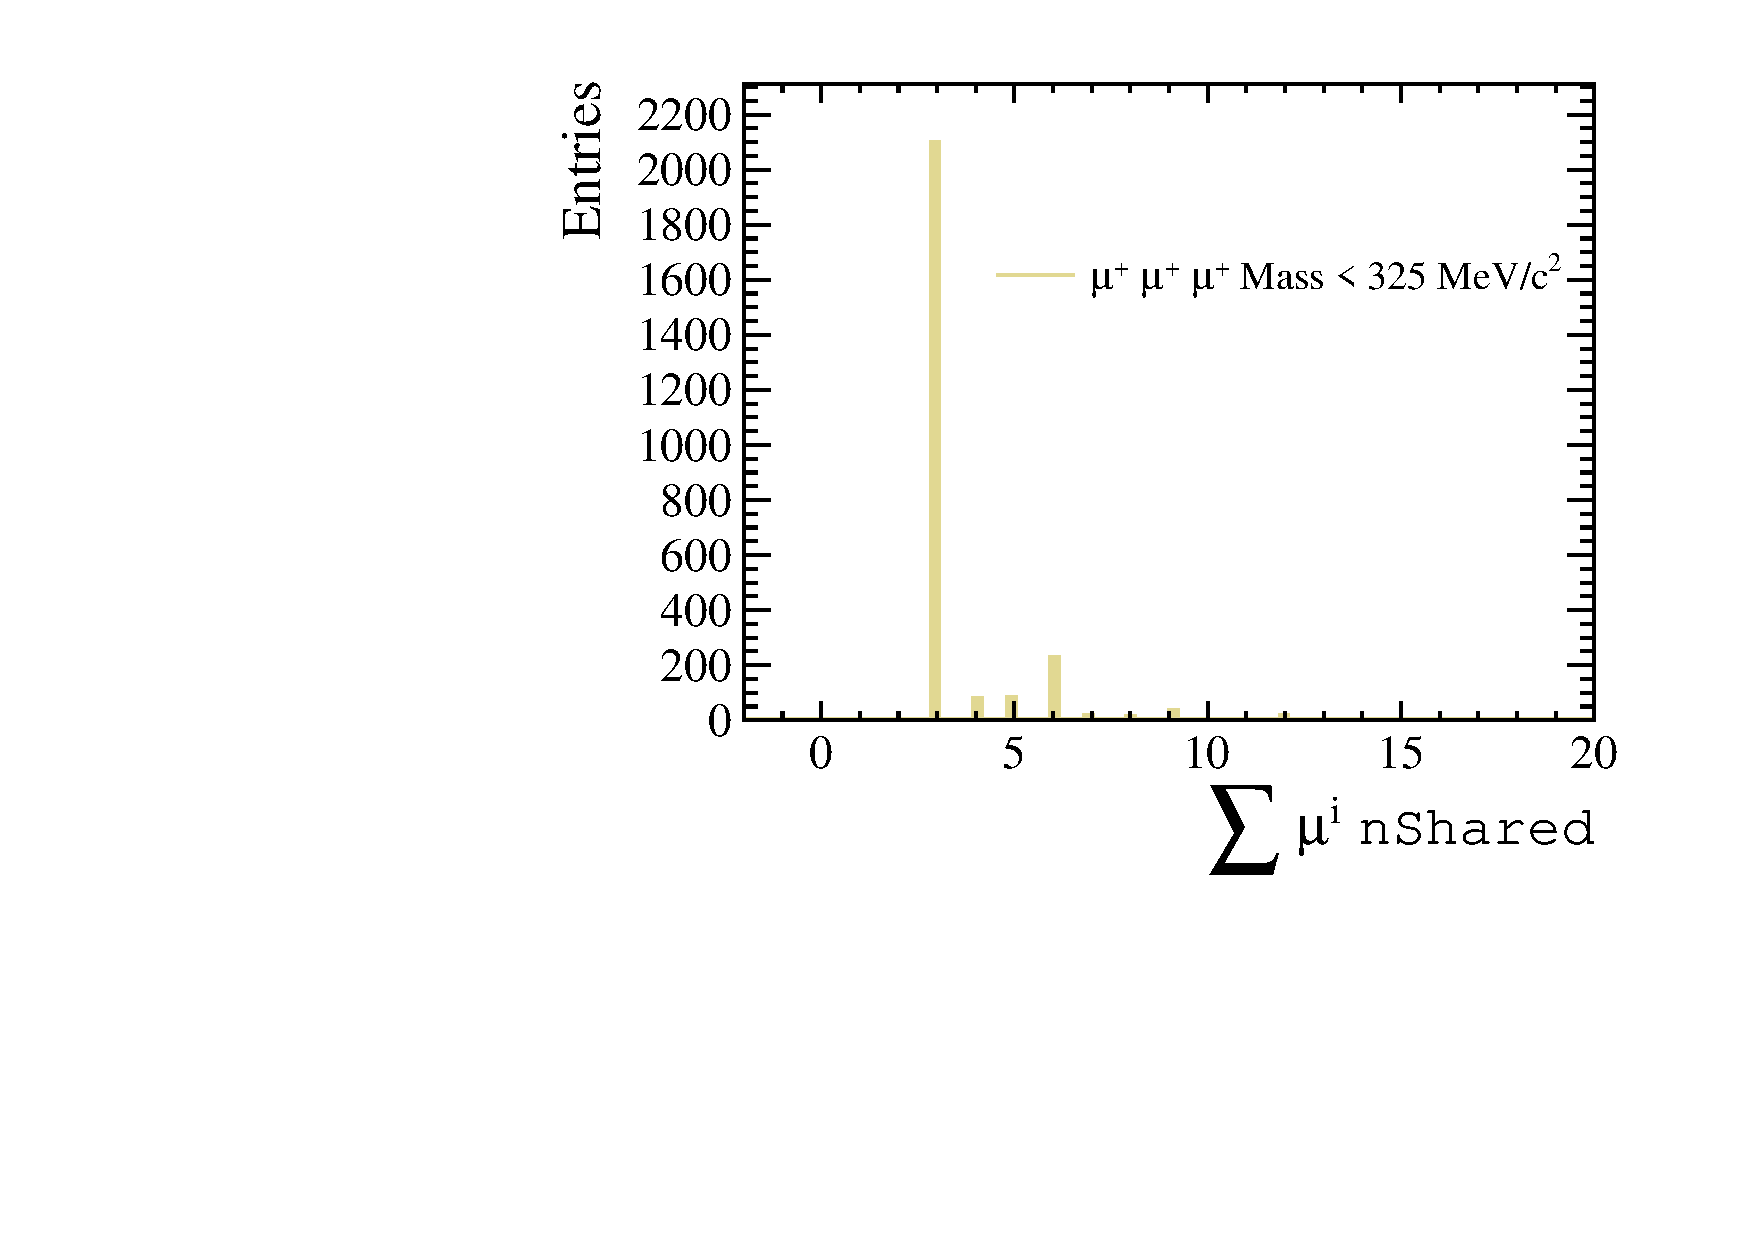
\includegraphics[width=0.5\linewidth]{trimuon/compnice_even_nicer_ONLY_STACKED_HIST_oneFILE_sumnSharedclone.pdf}\put(-50,133){(a)}
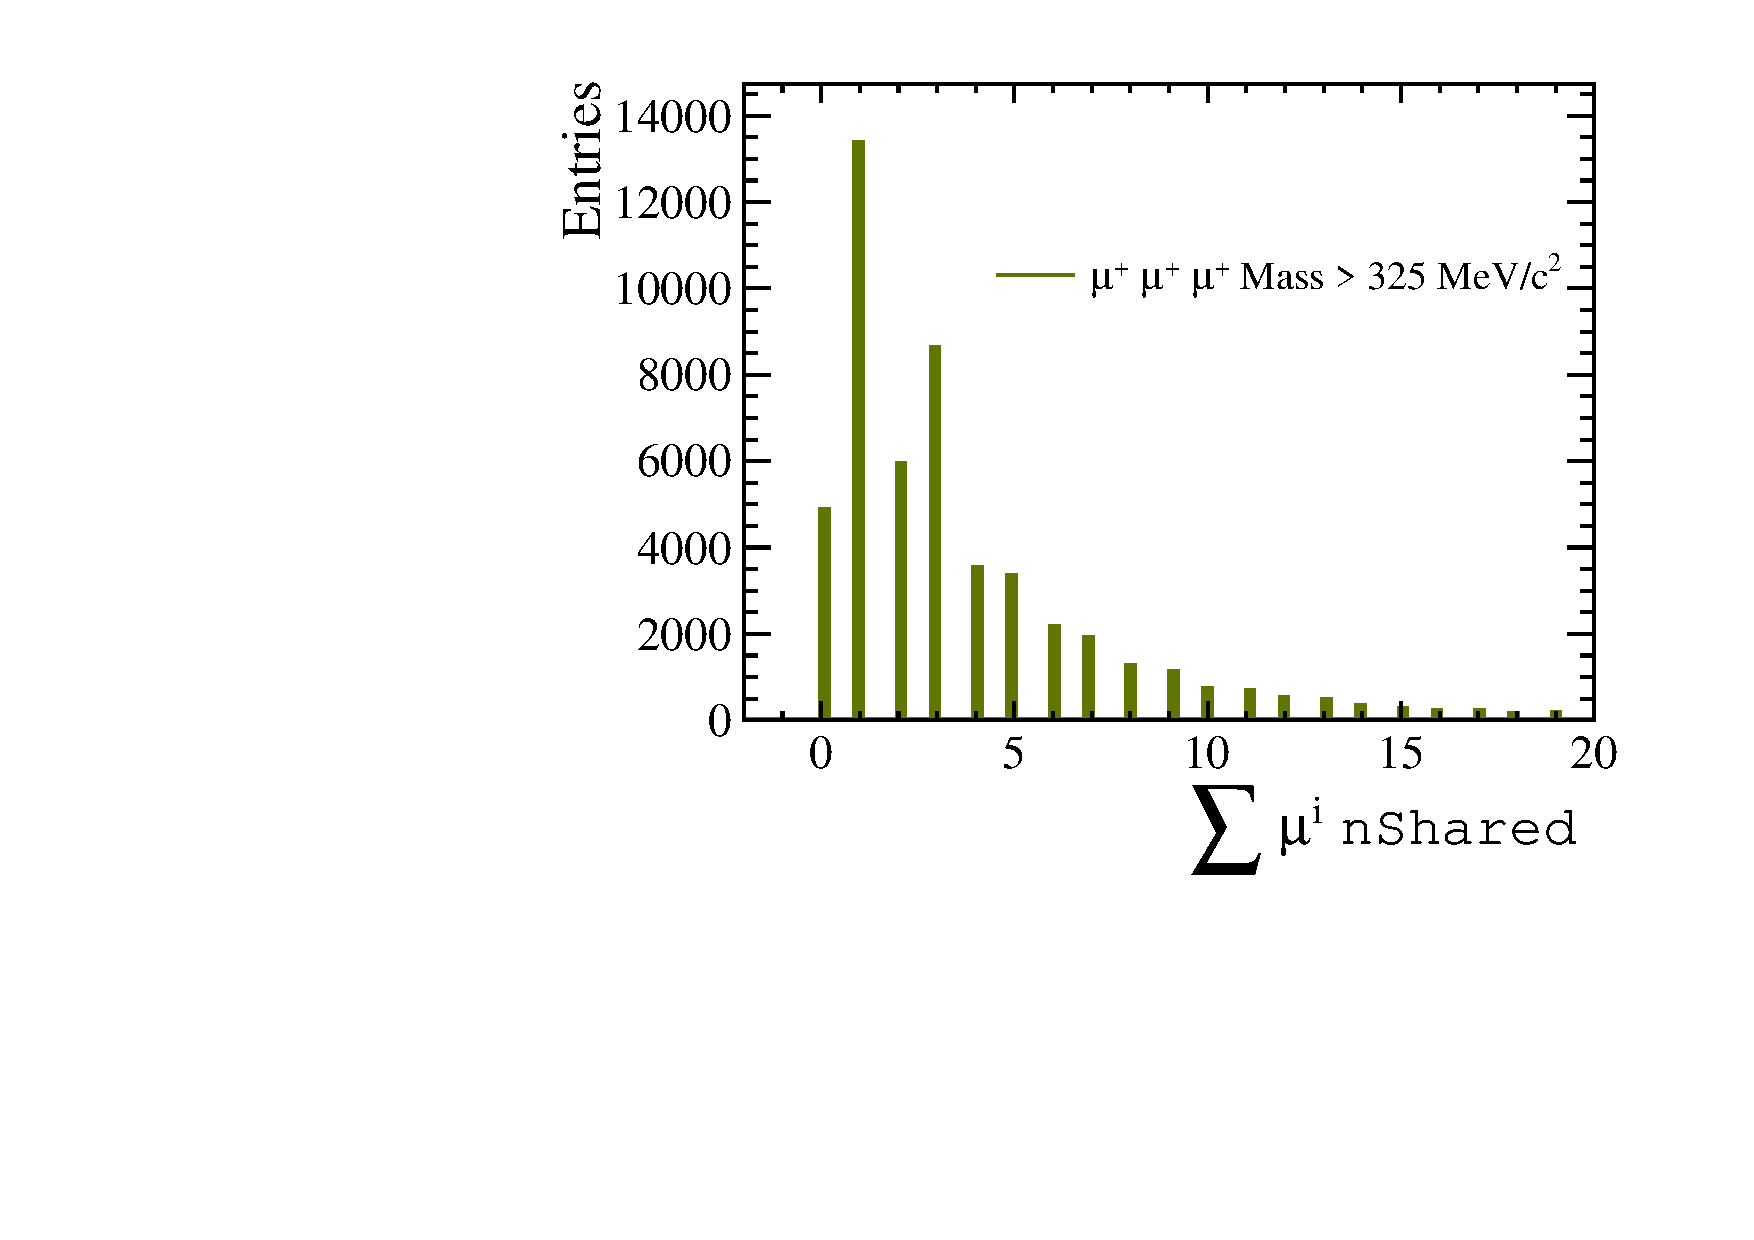
\includegraphics[width=0.5\linewidth]{trimuon/compnice_even_nicer_ONLY_STACKED_HIST_oneFILE_sumnSharednoclone.pdf}\put(-50,133){(b)}
	\caption{(a) Clone and (b) no clone distribution for sum of all muon \texttt{nShared}. Since in this case the clones are of each other, for the clones there is clear peak at three. }
\label{fig:ClonesnShared}
%\vspace*{-1.0cm}
\end{figure}

\section{Probability of \mb{K/\pi \rightarrow \mu} misidentification at LHCb }

Usually, in order to estimate background coming from misidentification of particles as muons in the detector, data samples with particles of known (non-muon) type are identified from the kinematics of the decay chains. From these samples, probabilities of mis-identification are derived as discussed in~\autoref{RICHperf}. However, the three muon signature will induce problems for \gls{PID} variables that are correlated with the number of muons in the detector and specific data samples that incorporates this correlation have to be used for measuring the mis-identification probability.

\subsection{Specific control sample for \mb{K/\pi \rightarrow \mu} misID rates }
\label{extraction}
A platform that \gls{LHCb} analysts usually use to extract the misID and id efficiencies, as described in~\autoref{RICHperf}, is known as the \texttt{PIDCalib} package \cite{Anderlini:2202412}. It contains samples where the identity of the particle is know purely from kinematics.  In this \texttt{PIDCalib} package, such a control same for $K/\pi$ is obtained from $D^{*+}(\rightarrow D^{0}(\rightarrow \underline{K^{+} \pi^{-}}) \pi^{+})$. These statistically populated background-free \textit{sWeighted} samples\cite{sPlot}, for which it is possible to extract misID and ID rates as a function of kinematics given certain \gls{PID} criteria, do not have other muons in the final state. 

More specifically, the topology of the mis-ID background component, which is two real muon tracks with an additional \textit{fake} muon track is very different to the \texttt{PIDCalib} sample $D^{*+}(\rightarrow D^{0}(\rightarrow \underline{K^{+} \pi^{-}}) \pi^{+})$, where there are no muons in the final state.

%This influences the rest of the misID rates as some of the \gls{PID} variables are strongly correlated with number of muons in the decay, due to the fact that the mis-identified particle can share hits with other muons in the rest of the decay. This should be reflected mostly in high momenta region, where the three particles tend to be collimated and share hits most often.

For this reason, $B^{0} \rightarrow J/\psi(\rightarrow \mu^{+} \mu^{-}) K^{*}(\rightarrow \underline{K^{+} \pi^{-}})$ is used instead. While not as common as $D^{*+}(\rightarrow D^{0}(\rightarrow \underline{K^{+} \pi^{-}}) \pi^{+})$ decay, it still has high statistics and can be isolated with little background. It mimics the two real muon plus fake muon correctly and will be used to obtain pion and kaon misID probabilities.
% This is a clean decay that can be fit to obtain \textit{sWeights} to measure PID efficiencies. Moreover, its the signal topology and kinematics are much closer to the actual mis-ID backgroundcomponent than
% that of the PIDCalib control samples.

\subsection{Selection for \mb{B^{0} \rightarrow J/\psi(\rightarrow \mu^{+} \mu^{-}) K^{*}}  }
Data samples for each year of data taking were obtained from the \textit{stripping line} dedicated to look for this type of decay. The sample can be used for mis-ID studies of the hadrons as no particle identification is applied on them. Some initial selection was applied together with the more stringent \Bmumumu selection.  The trigger criteria were applied on the $J/\psi$ candidate rather than on the $B$ candidate. The full additional selection is summarized in Table ~\ref{tab:cleanjpsikst} is used.


\begin{table}[h!]
\begin{center}
\begin{tabular}{ l  l }
\toprule
Idea  & Cut  \\ \hline
ID $K^{*}$ & $|$ M(K$\pi$) - M$_{PDG}(K^{∗}_{0})$ $|$ $ <100$ \mevcc \\
%Compatible with \texttt{PIDCalib} & \color{black} &  for K,$\pi$ , p$_{T} > 250$ \mevc\\
%Compatible with \texttt{PIDCalib} &  for $\mu$ , p$_{T} > 800$ \mevc \\
Muon swap veto & $|$ M((h $\rightarrow \mu$ )$\mu$) - M$_{PDG}$(J/$\psi$)$|$ $> 60$ \mevcc \\
	Veto $B^{+}\rightarrow K^{+}\mu^{+}\mu^{-}$ & max(M($K^{+}\mu^{+}\mu^{-}$)), M($(\pi^{+} \rightarrow K^{+})\mu^{+}\mu^{-})$) $< 5100$ \mevcc\\
Veto $B^{0}_{s}\rightarrow \phi \mu^{+} \mu^{-} $ & M(K($\pi\rightarrow$ K)) $>1040$ \mevcc \\
	ID muons & \texttt{Probnnmu}$>$0.5 \\
\hline
For kaon misID rates: & \\
ID pion & DLLK $<$ 0 DLLp $<$ 0 and \texttt{IsMuon==0}\\
\hline
For pion misID rates: & \\
ID kaon & DLLK $>$ 0 and DLLK-DLLp $>$ 0 and \texttt{IsMuon==0} \\
\bottomrule
\end{tabular}
\end{center}
\caption{Offline selection for $B^{0} \rightarrow J/\psi(\rightarrow \mu^{+} \mu^{-}) K^{*}$ decay.}
\label{tab:cleanjpsikst}
\end{table}


\subsection{Fitting Strategy for \mb{B^{0} \rightarrow J/\psi(\rightarrow \mu^{+} \mu^{-}) K^{*}} decay }
After the selection, the residual background needs to be modelled. The signal component, $B^{0} \rightarrow J/\psi K^{*}$, is obtained by fixing the shape from simulation apart from the mean $\mu$ and the width $\sigma$. It is fitted with a double-sided Hypatia function \cite{Santos:2013gra} (more in~\autoref{IP}).

Background that peaks in the upper mass sideband, coming from heavier $B^{0}_{s}$, $\bar{B}^{0}_{s} \rightarrow J/\psi (\rightarrow \mu^{+} \mu^{-}) K^*(\rightarrow \underline{K^{+} \pi^{-}})$ is also modelled using simulation, using the same function as signal but with $\mu$ offset by the difference between the known $B^{0}_{s}$ and $B^{0}$.

It is also possible that kaons and pions are swapped between themselves. Background coming from $K \leftrightarrow \pi$ swaps is modelled from simulation where the mass hypotheses were swapped. Its distribution is fitted with a double sided Crystal Ball function \cite{Skwarnicki:1986xj} (more in~\autoref{CB}).

Possibility of misidentified background comes from decay of $\Lambda_{b} \rightarrow K^{-} p \mu^{+} \mu^{-}$ where the proton is misidentified as a pion. This background is modelled from simulation and fitted with a \texttt{RooKeys} p.d.f (more in~\autoref{RK}).

Finally a combinatorial component is modelled by the exponential function.


The mass of the $J/\psi$ was \textit{constrained} to its nominal mass, a procedure also known as a \textit{mass constraint}. It yields new estimates for track parameters of the final state particles, from which a new kinematic refit is done.

In order to obtain $K/\pi$ misID probabilities an unbinned maximum likelihood fit to the $\mu^{+} \mu^{-} \pi^{+} K^{-}$ mass between 5150 - 5450 \mevcc was performed. This fit with parameters listed in~\autoref{tab:floatingparsummarylol} give the yield of all the components. 

\begin{table}[H]
\centering
\begin{tabular}{ l  l }\toprule
Fit Parameter & Status  \\ \hline
	\multicolumn{2}{c}{Yields} \\ \hline
$N_{B^{0} \rightarrow J/\psi K^{*}}$ (Signal)  &  Free \\
$N_{K \pi swaps}$ & Free\\
$N_{\Lambda_{b} \rightarrow J/\psi K^{-} p}$ & Free\\
$N_{B_{s} \rightarrow J/\psi K^{*}}$ & Free \\
$N_{Combinatorial}$ & Free\\
\hline
	\multicolumn{2}{c}{Signal Shape Parameters} \\
\hline
$\mu_{B^{0} \rightarrow J/\psi K^{*}}$ & Constrained from signal MC\\
$\sigma_{B^{0} \rightarrow J/\psi K^{*}}$ & Constrained from signal MC\\
Others & Fixed from MC\\
\hline
$K\ \pi\ swaps$ Shape Parameters & Fixed from MC \\
\hline
$\Lambda_{b} \rightarrow J/\psi K^{-} p$ Shape Parameters & Fixed from MC \\
\hline
	\multicolumn{2}{c}{${B_{s} \rightarrow J/\psi K^{*}}$ Shape Parameters} \\\hline
$\mu_{B_{s} \rightarrow J/\psi K^{*}}$ & Offset by $\mu_{B^{0} \rightarrow J/\psi K^{*}}$ \\
Others & Fixed from signal MC \\
\hline
	\multicolumn{2}{c}{Combinatorial Shape Parameters}  \\
\hline
exponential par.  & Free\\
\bottomrule
\end{tabular}
\caption{Summary of the fit parameters and individual component constraints for $B^{0} \rightarrow J/\psi K^{*}$ fit.}
\label{tab:floatingparsummarylol}
\end{table}






The actual determination of the misID rate was obtained using a statistical method of background subtraction, known as the \textit{sPlot} technique \cite{sPlot}, as the samples are not fully background-free. The same method is also used in the \texttt{PIDCalib} package. In the \textit{sPlot} method, the invariant mass distribution is fitted with no \gls{PID} applied and each event is assigned \textit{sWeights}, probabilities that a given event is a signal-like or a background-like. Then, through the \textit{sPlot} technique, background is subtracted. Signal component can then be calculated by summing all the \textit{sWeights} for all the candidates. The misID probabilities are finally obtained by dividing this signal component sum of \textit{sWeights} with \gls{PID} applied and with no \gls{PID} applied. This misID probabilities are then considered within some kinematic partitioning, bins of $p,\eta$. 

\color{black}

The misID rate was also cross-checked with another method, the \textit{fit twice method}. This is because the \textit{sPlot} technique relies on the fact that there is no correlation between the control variables ($p$, $\eta$) and the discriminating variable (invariant mass) for both signal and background. This assumption may not be true, especially for background, and it can introduce biases.

The \textit{fit twice method} consists of fitting $B^{0} \rightarrow J/\psi(\rightarrow \mu^{+} \mu^{-}) K^{*}$ before and after the \gls{PID} requirement in a given kinematic ($p$, $\eta$) bin separately. Misid probabilities are then obtained as the ratio of signal yields arising from these two fits.


It was shown that these two methods yields very similar results, hence,
for purposes of the \Bmumumu analysis the \textit{sWeight} values will be used. Fits to Run \Rn{1} and Run \Rn{2} data for both kaon and pion misID studies can be seen in ~\autoref{fig:JpsiKst}.
%IF YOU WANT TO CHANGE THE PLOTS HAVE A LOOKHERE /vols/lhcb/ss4314/fitjpsikst/fitjpsikst_idKAON_includeswaps_automatize_master_sweight_cinMuonAc_NOghostprob_mydefbin_onnlyONEbinINeta_2016_newPIDopt/NOFCME/ there is mainPLOTonly function
\begin{figure}[H] 

\center
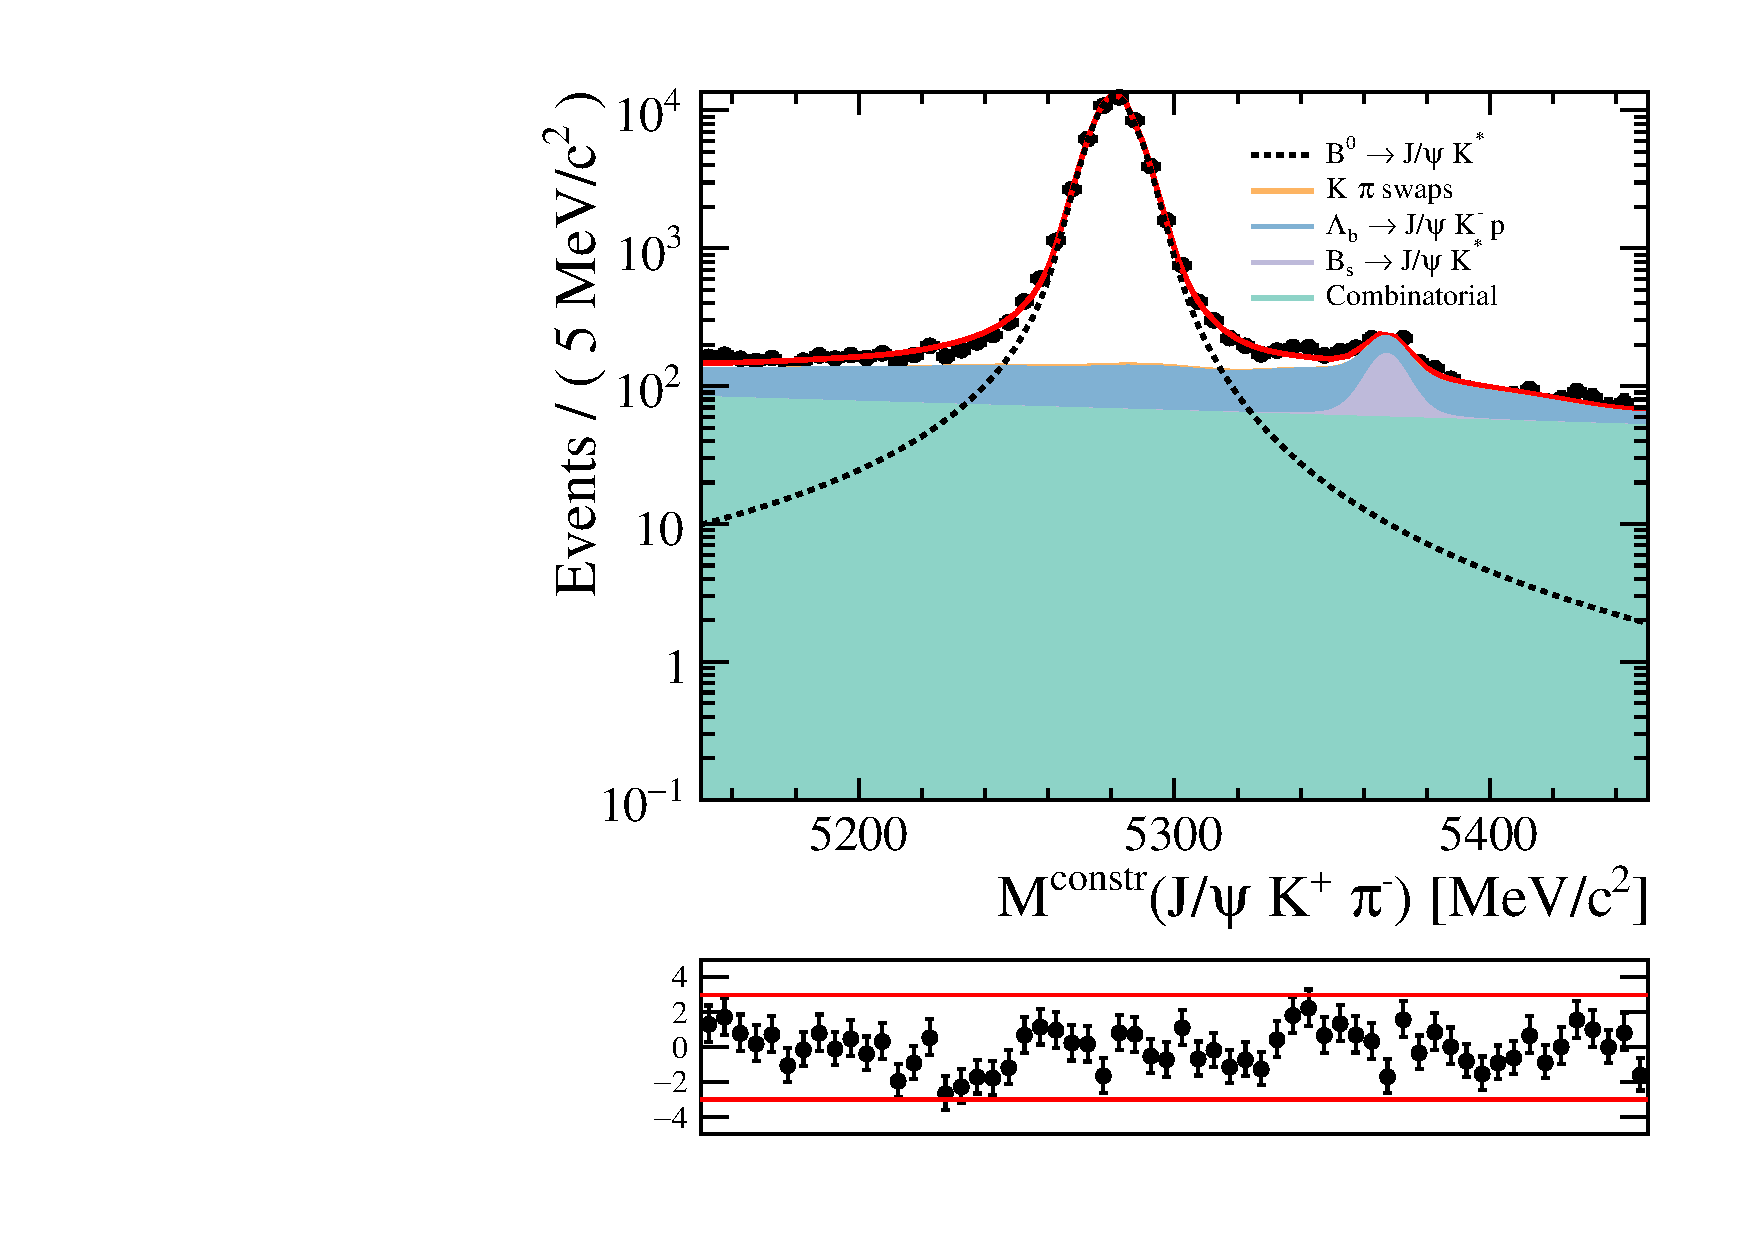
\includegraphics[width = 0.5\textwidth]{figs/trimuon/jpsikst/2011/plotJpsiKstFitLogyPretty_nicecolor_2011_KAONMISID.pdf}\put(-150,100){(a) 49K events }%
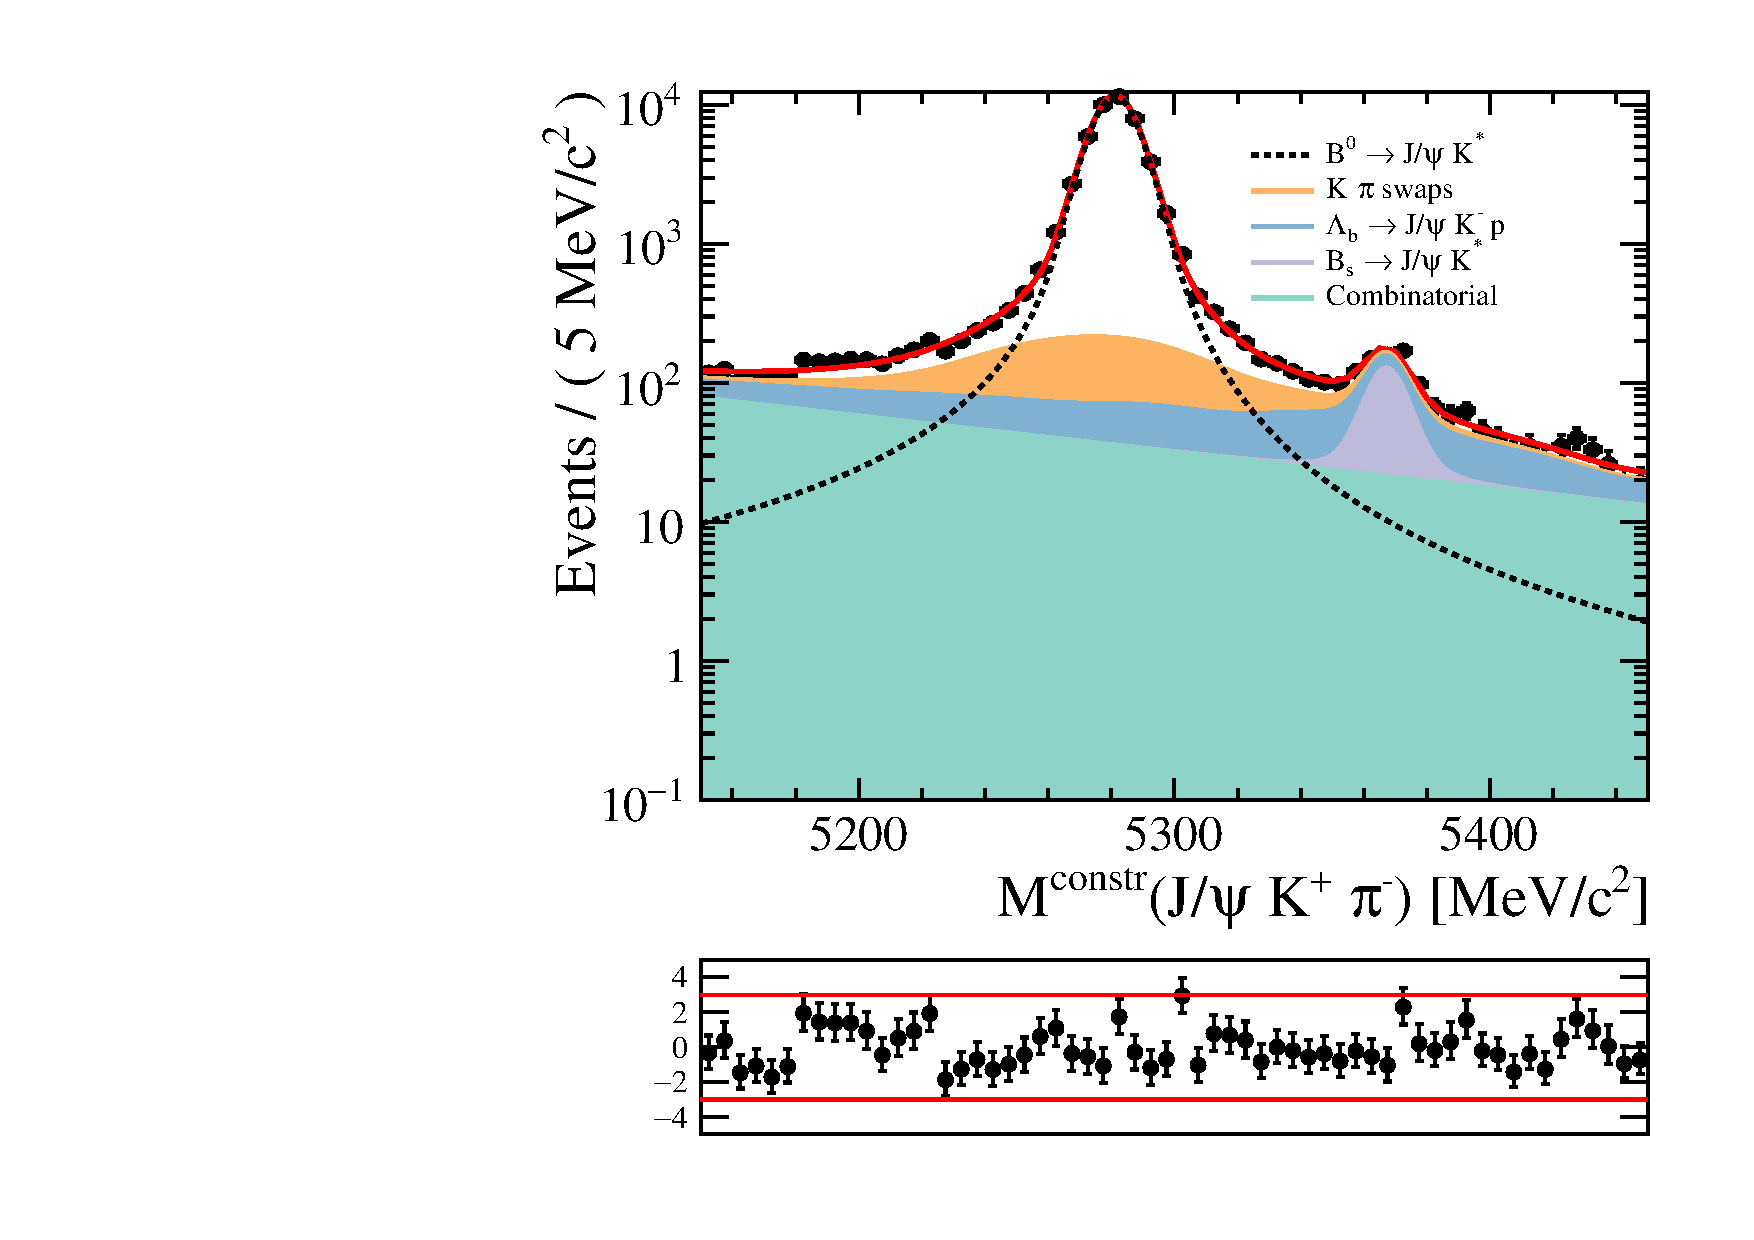
\includegraphics[width = 0.5\textwidth]{figs/trimuon/jpsikst/2011/plotJpsiKstFitLogyPretty_nicecolor_2011_PIONMISID.pdf}\put(-150,100){(b) 46K events}
\newline
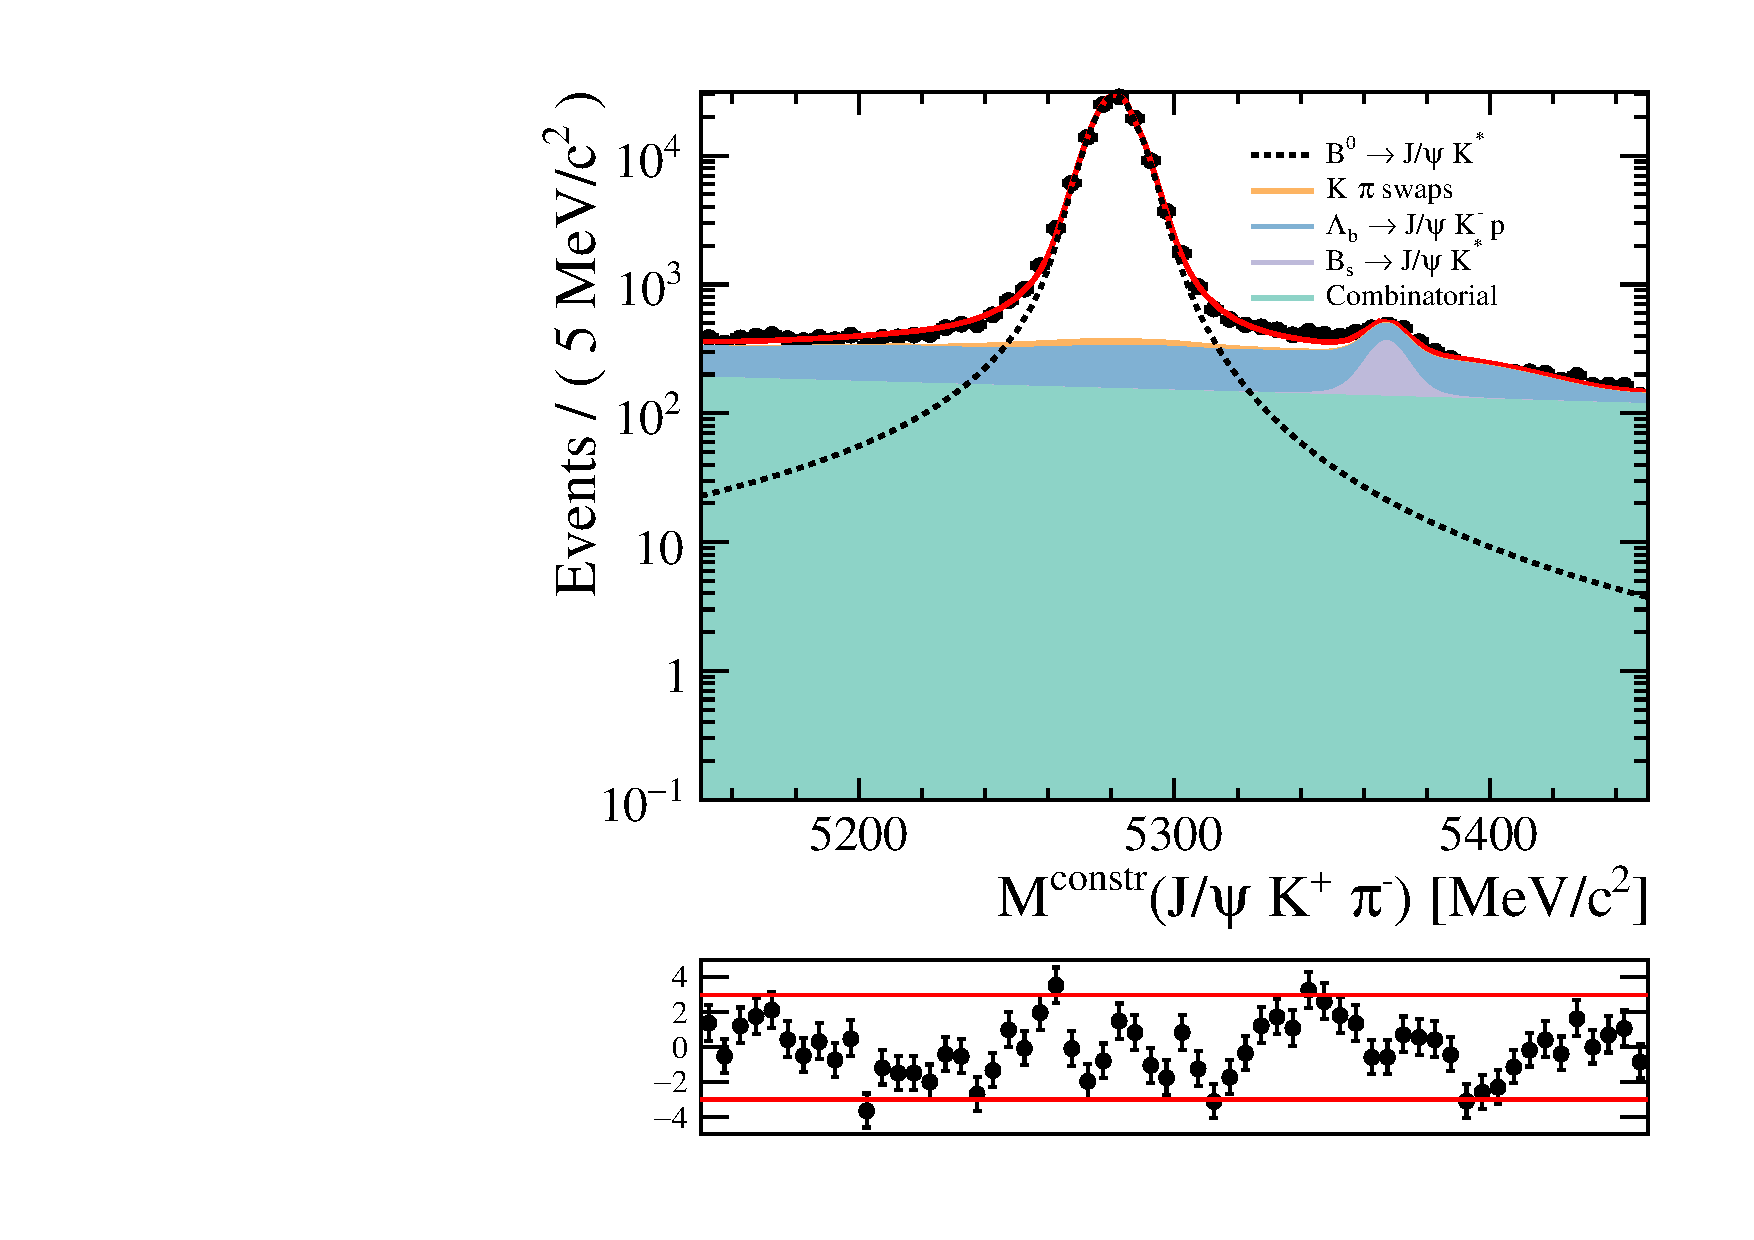
\includegraphics[width = 0.5\textwidth]{figs/trimuon/jpsikst/2012/plotJpsiKstFitLogyPretty_nicecolor_2012_KAONMISID.pdf}\put(-150,100){(c) 112K events }%
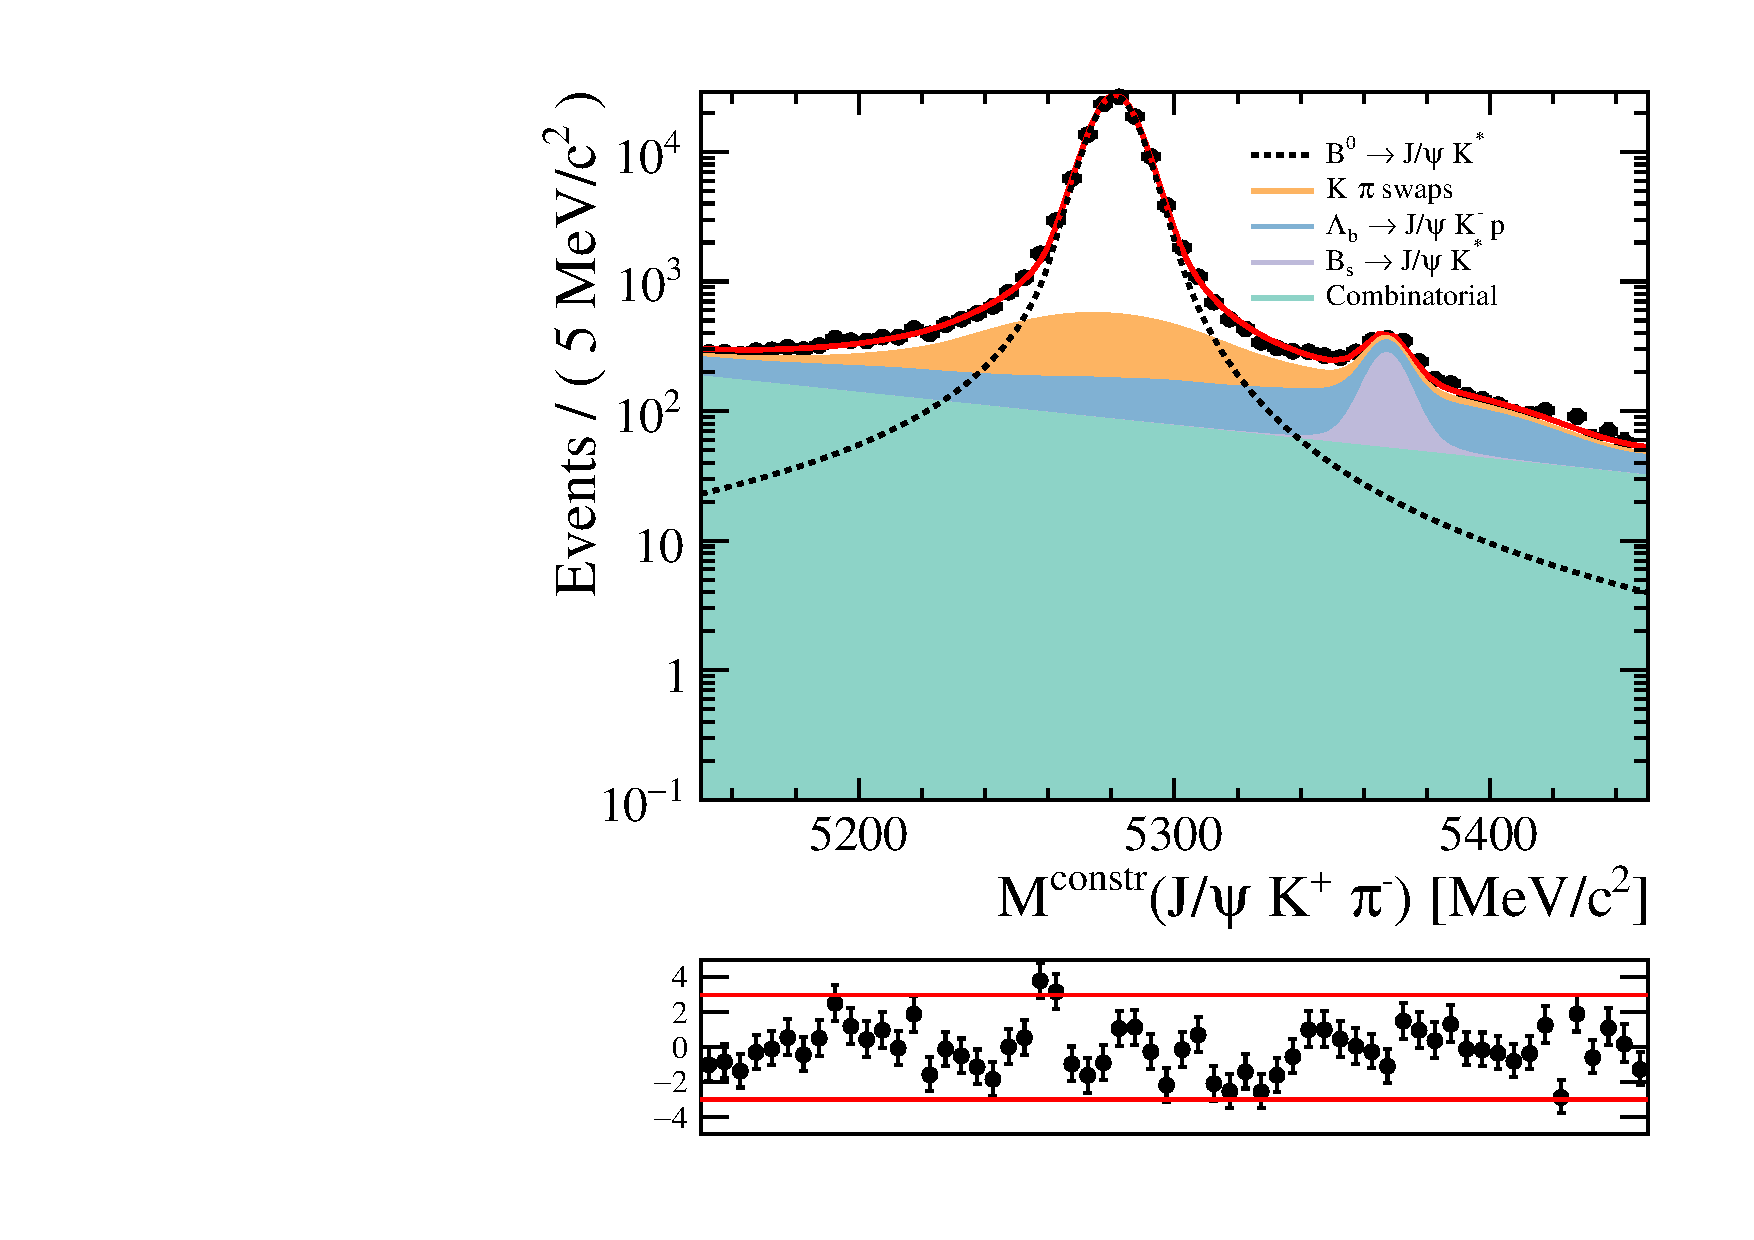
\includegraphics[width = 0.5\textwidth]{figs/trimuon/jpsikst/2012/plotJpsiKstFitLogyPretty_nicecolor_2012_PIONMISID.pdf}\put(-150,100){(d) 107K events}
\newline
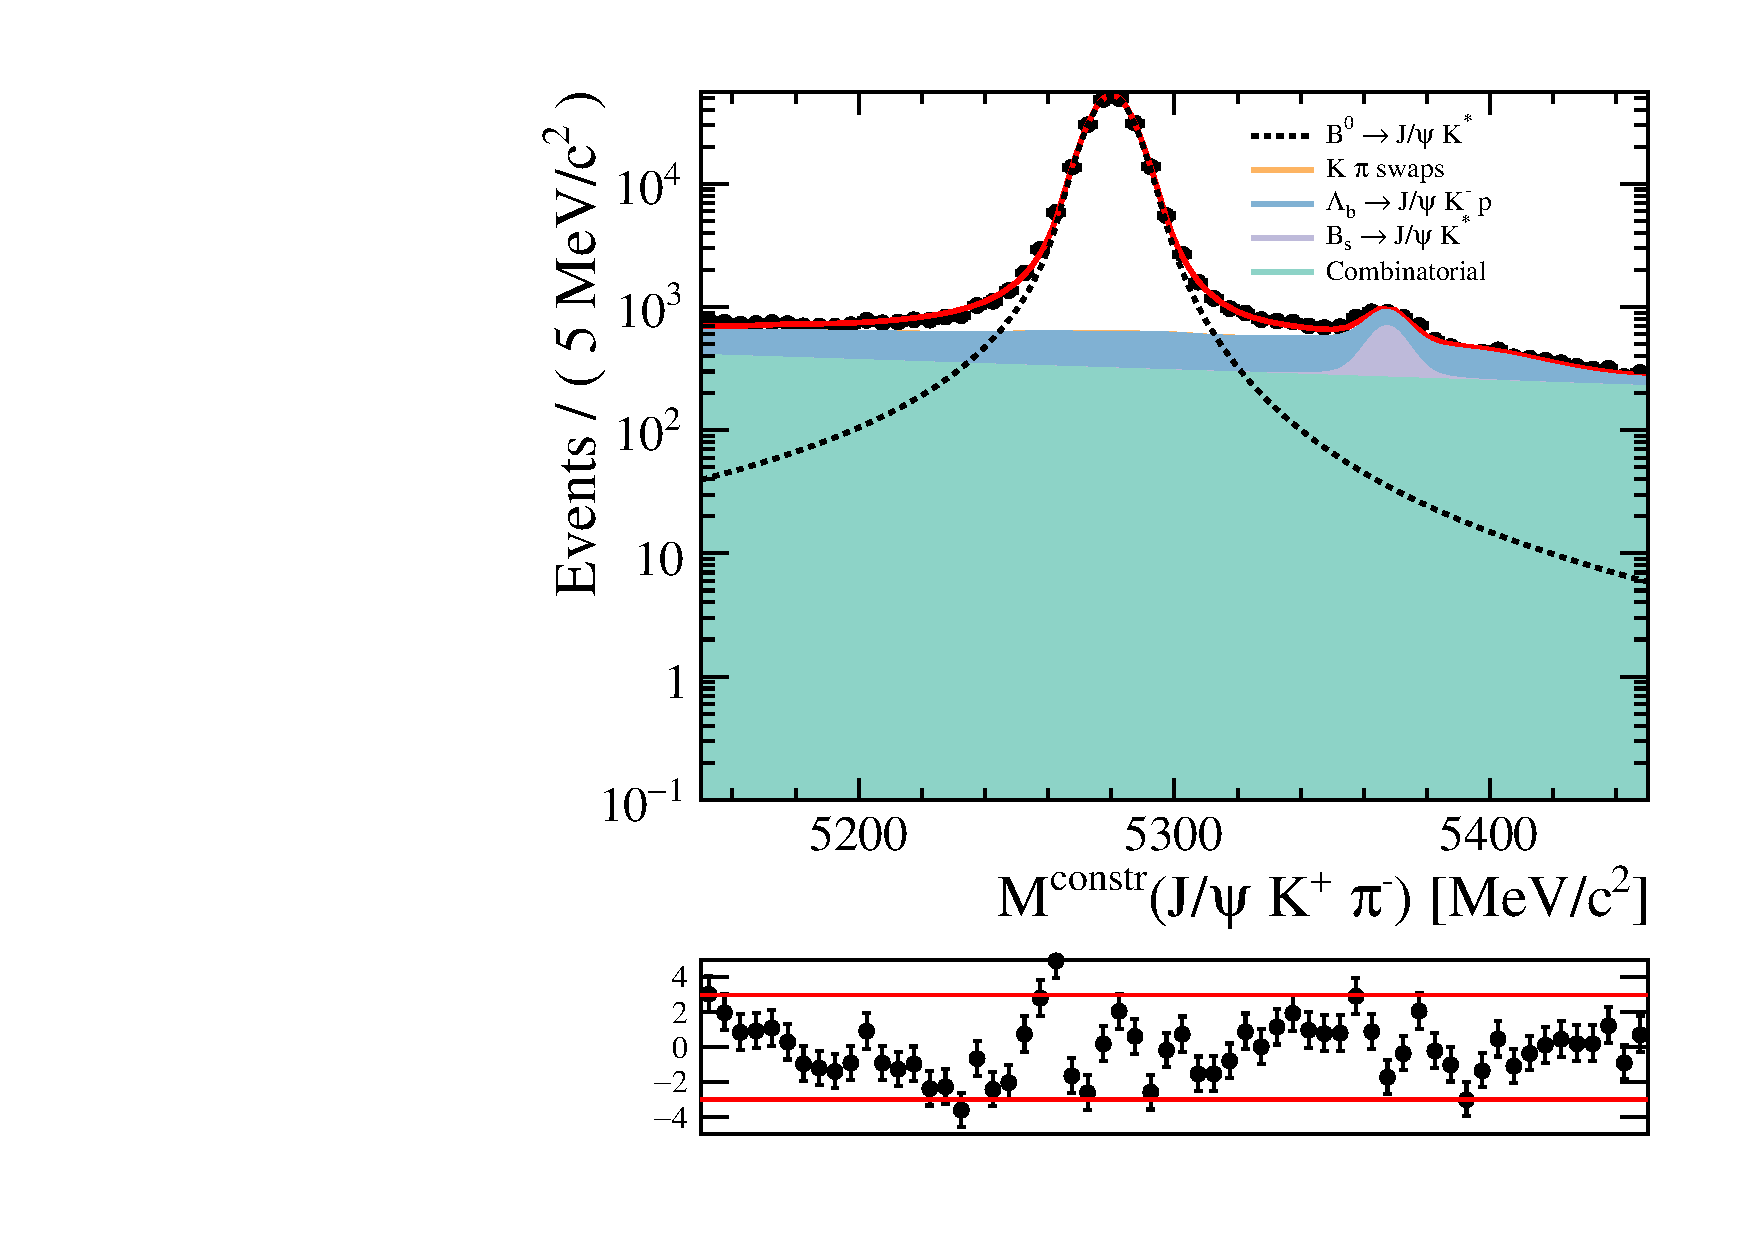
\includegraphics[width = 0.5\textwidth]{figs/trimuon/jpsikst/2016/plotJpsiKstFitLogyPretty_nicecolor_2016_KAONMISID.pdf}\put(-150,100){(e) 205K events}%
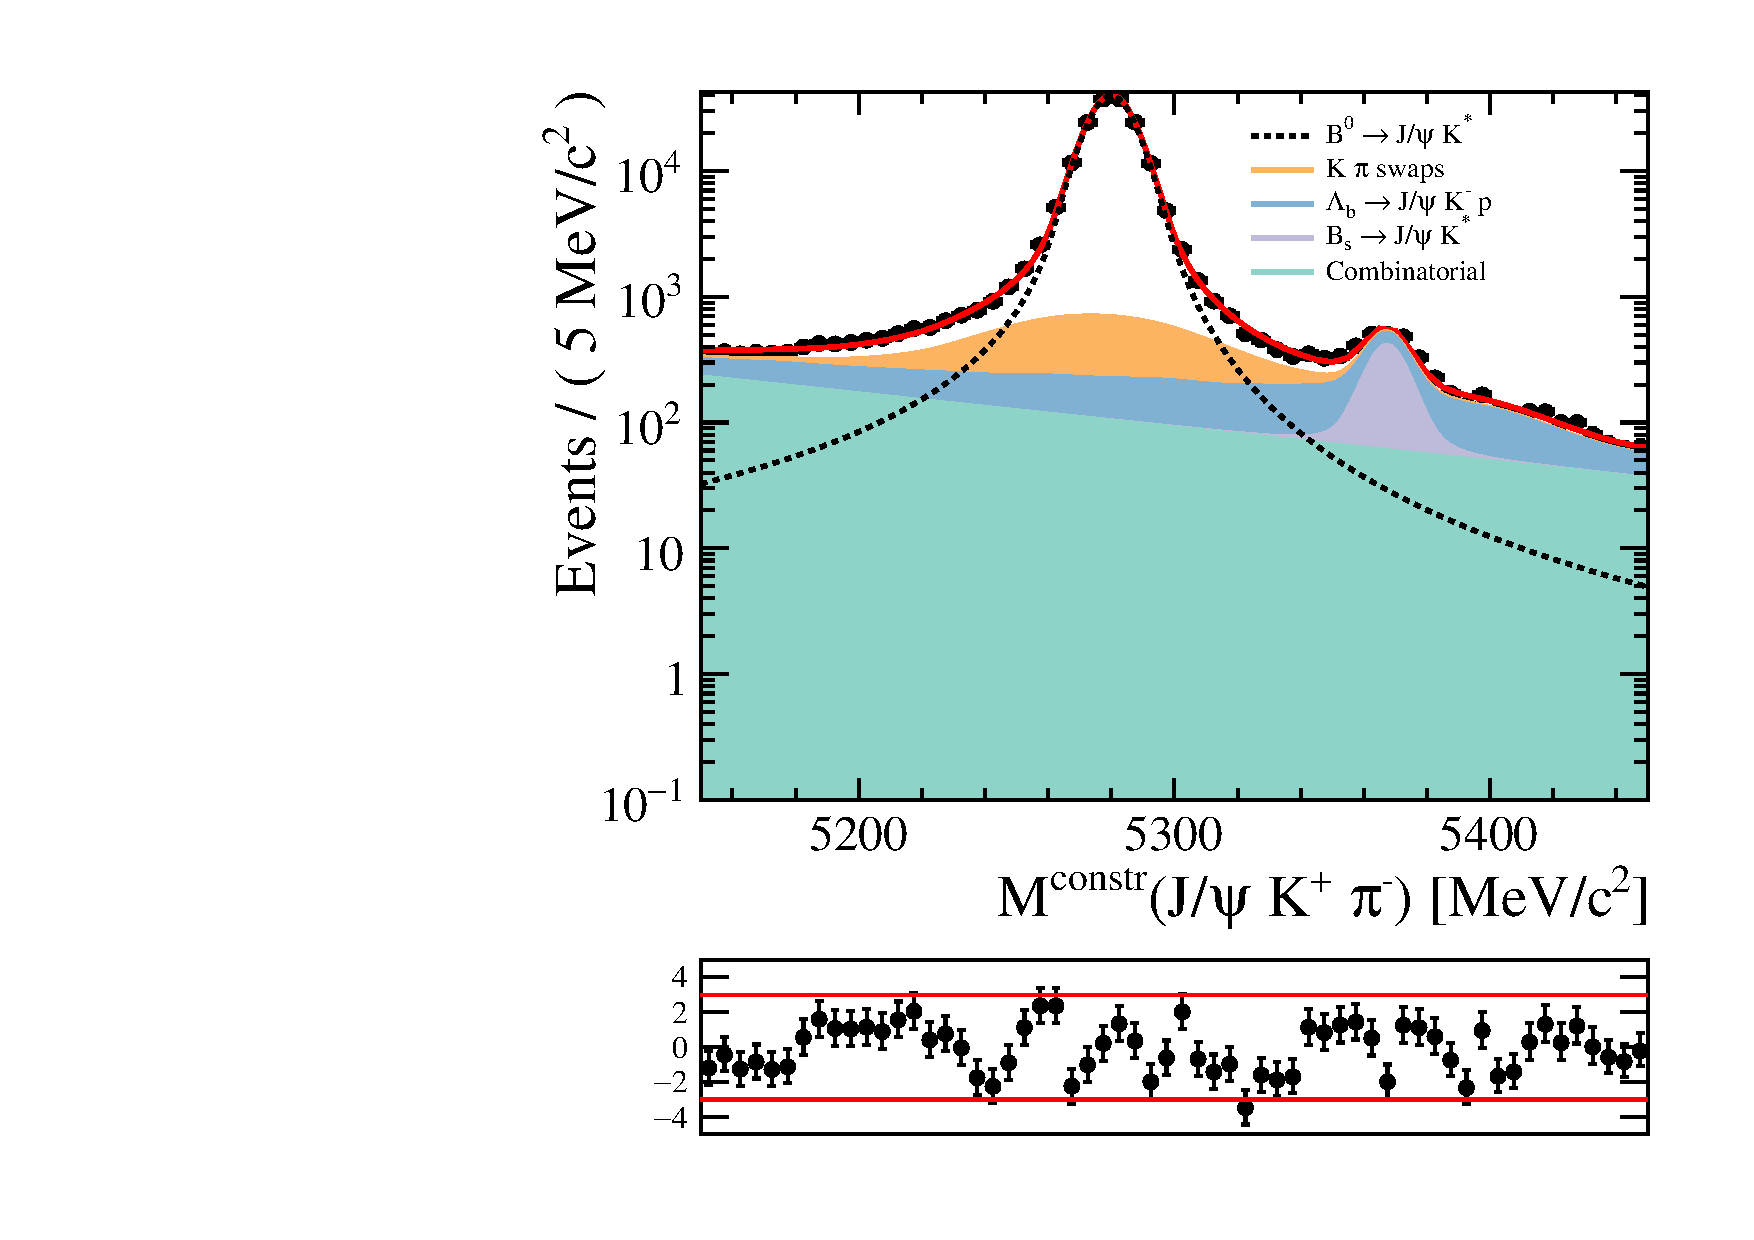
\includegraphics[width = 0.5\textwidth]{figs/trimuon/jpsikst/2016/plotJpsiKstFitLogyPretty_nicecolor_2016_PIONMISID.pdf}\put(-150,100){(f) 161K events}
	\caption{Fit to constrained $J/\psi(\rightarrow \mu^{+} \mu^{-}) K^{*}(\rightarrow \pi^{+} K^{-})$ mass with all the components for (a)(b) 2011, (c)(d) 2012, (e)(f) 2016. On the left, fit to data with pion ID (giving kaon misID probabilities), on right data with kaon ID (pion misID rates).}
\label{fig:JpsiKst}
\end{figure}

\subsection{Results of \mb{B^{0} \rightarrow J/\psi(\rightarrow \mu^{+} \mu^{-}) K^{*}} control sample for \mb{K/\pi \rightarrow \mu} misID rates }
\label{ratiatkos}
%\color{red} Using the \textit{sWeight} method, misID rates for kaons and pions can be obtained. In order to rule out that any disagreement of \gls{PID} performance is caused by the fraction of the real kaon and pions tracks within the muon fiducial area, following check is performed. For both control samples, kaon sample from the $D^{*+}(\rightarrow D^{0}(\rightarrow \underline{K^{+} \pi^{-}}) \pi^{+})$ events and the kaon sample from the $B^{0} \rightarrow J/\psi(\rightarrow \mu^{+} \mu^{-}) K^{*}$ events, the probability of correctly identifying kaon is computed, given that only extrapolated tracks that fall within muon acceptance are considered. This is achieved by requiring that given kaon track has \texttt{InMuonAcceptance==1.0}. It can be seen in ~\autoref{tab:ROE} that the ID performance is the same across nearly all of the momentum range for kaons, showing that the fraction of the kaons tracks within muon acceptance is very similar. The same check was performed for pions tracks as well. 

%\color{black}
%
%\begin{table}[h!]
%%\small
%\begin{center}
%\begin{tabular}{ l  H  H  c   }\toprule
%	$p$ range [\mevc] & $D^{*+}(\rightarrow D^{0}(\rightarrow \underline{K^{+} \pi^{-}}) \pi^{+})$  & $B^{0} \rightarrow J/\psi(\rightarrow \mu^{+} \mu^{-}) K^{*}(\rightarrow \underline{K^{+} \pi^{-}})$  & $B^{0} \rightarrow J/\psi(\rightarrow \mu^{+} \mu^{-}) K^{*}(\rightarrow \underline{K^{+} \pi^{-}})/D^{*+}(\rightarrow D^{0}(\rightarrow \underline{K^{+} \pi^{-}}) \pi^{+})$  \\	
%\hline
%3000 - 6000 &   0.77$\pm$0.0016 & 0.83$\pm$0.0047 & 1.1$\pm$0.0065 \\
%6000 - 9300 &   0.93$\pm$0.00030 & 0.95$\pm$0.0019 & 1.0$\pm$0.0020 \\
%9300 - 10000 &  0.96$\pm$0.00037 & 0.97$\pm$0.0031 & 1.0$\pm$0.0033 \\
%10000 - 12600 &  0.97$\pm$0.00014 & 0.97$\pm$0.0017 & 1.0$\pm$0.0017 \\
%12600 - 15600 &   0.98$\pm$0.00011 & 0.97$\pm$0.0017 & 0.99$\pm$0.0018 \\
%15600 - 17500 &   0.98$\pm$0.00013 & 0.96$\pm$0.0024 & 0.98$\pm$0.0025 \\
%17500 - 21500 &   0.98$\pm$8.9e-05 & 0.96$\pm$0.0018 & 0.98$\pm$0.0018 \\
%21500 - 27000 &   0.98$\pm$7.8e-05 & 0.96$\pm$0.0018 & 0.98$\pm$0.0019 \\
%27000 - 32000 &   0.98$\pm$8.8e-05 & 0.96$\pm$0.0024 & 0.98$\pm$0.0025 \\
%32000 - 40000 &  0.98$\pm$8.0e-05 & 0.96$\pm$0.0022 & 0.98$\pm$0.0022 \\
%40000 - 60000 &  0.97$\pm$7.5e-05 & 0.95$\pm$0.0021 & 1.0$\pm$0.0022 \\
%60000 - 70000 &  0.96$\pm$0.00016 & 0.96$\pm$0.0043 & 1.0$\pm$0.0046 \\
%70000 - 100000 &  0.95$\pm$0.00013 & 0.94$\pm$0.0044 & 0.99$\pm$0.0046 \\
%\bottomrule
%\end{tabular}
%\end{center}
%	\caption{\color{red} It is necesarry as this is unrelated to following figures  \color{black}\texttt{K$\_$InMuonAcc==1.0} shows the interpolation of $K$ tracks into muon chambers. It can be seen that both samples agree with each other very well, meaning that measured misID rate is done for the same fraction of considered tracks. This measurement is done in a pseudorapidity region $1.5<\eta<5.0$.}
%\label{tab:ROE}
%\end{table}

Using the \textit{sWeight} method, misID rates for kaons and pions can be obtained. Two control samples that are analysed and compared are $D^{*+}(\rightarrow D^{0}(\rightarrow \underline{K^{+} \pi^{-}}) \pi^{+})$ events (standard \texttt{PIDCalib} sample), where there are no other muons in the decay, and $B^{0} \rightarrow J/\psi(\rightarrow \mu^{+} \mu^{-}) K^{*}(\rightarrow \underline{K^{+}\pi^{-}})$ events, where there are two real muons along with kaons or pions. Selecting only tracks that are within the muon fiducial region for both pion and kaon allows to perform study of the misID probabilities within the two calibration samples. In ~\autoref{fig:JpsiKnew}(a), the $\pi \rightarrow \mu$ misID probability for different \gls{PID} hypotheses from $B^{0} \rightarrow J/\psi(\rightarrow \mu^{+} \mu^{-}) K^{*}(\rightarrow K^{+}\pi^{-})$ sample is studied. As it can be noticed, the more stringent the muon selection on the pion track, the lower the probability of misidentification.

In general the agreement between the two samples is good in the low momentum regions as shown in ~\autoref{fig:JpsiKnew}(b). These pions are softer and hence they will spread out more in the magnetic field, causing less interference with two other real muons in decay. However, in the high momentum region, the pion will follow a path through the muon system that is more similar to the path of the muon of the same charge in the $B^{0} \rightarrow J/\psi(\rightarrow \mu^{+} \mu^{-}) K^{*}$ decay. The influence of the two other real muons in a high momenta the region will lead to bigger disagreement as these two real muons leave hits in the muon chambers close to the collimated pion track, making the rate of \texttt{IsMuon==1.0} (pink) higher. 


%By selection tracks within the muon fiducial region for both pion and kaon allows to perform study of the misID probabilities with the two calibration samples.
%In ~\autoref{fig:JpsiKnew}, the $\pi \rightarrow \mu$ misID probability for different \gls{PID} hypotheses are studied. As it can be noticed, the more stringent the muon selection on the pion track, the lower the probability of misidentification. 

%On the right, the ratio of the misID probabilities between two samples show particular trend. 


\begin{figure}[h!]
\center
%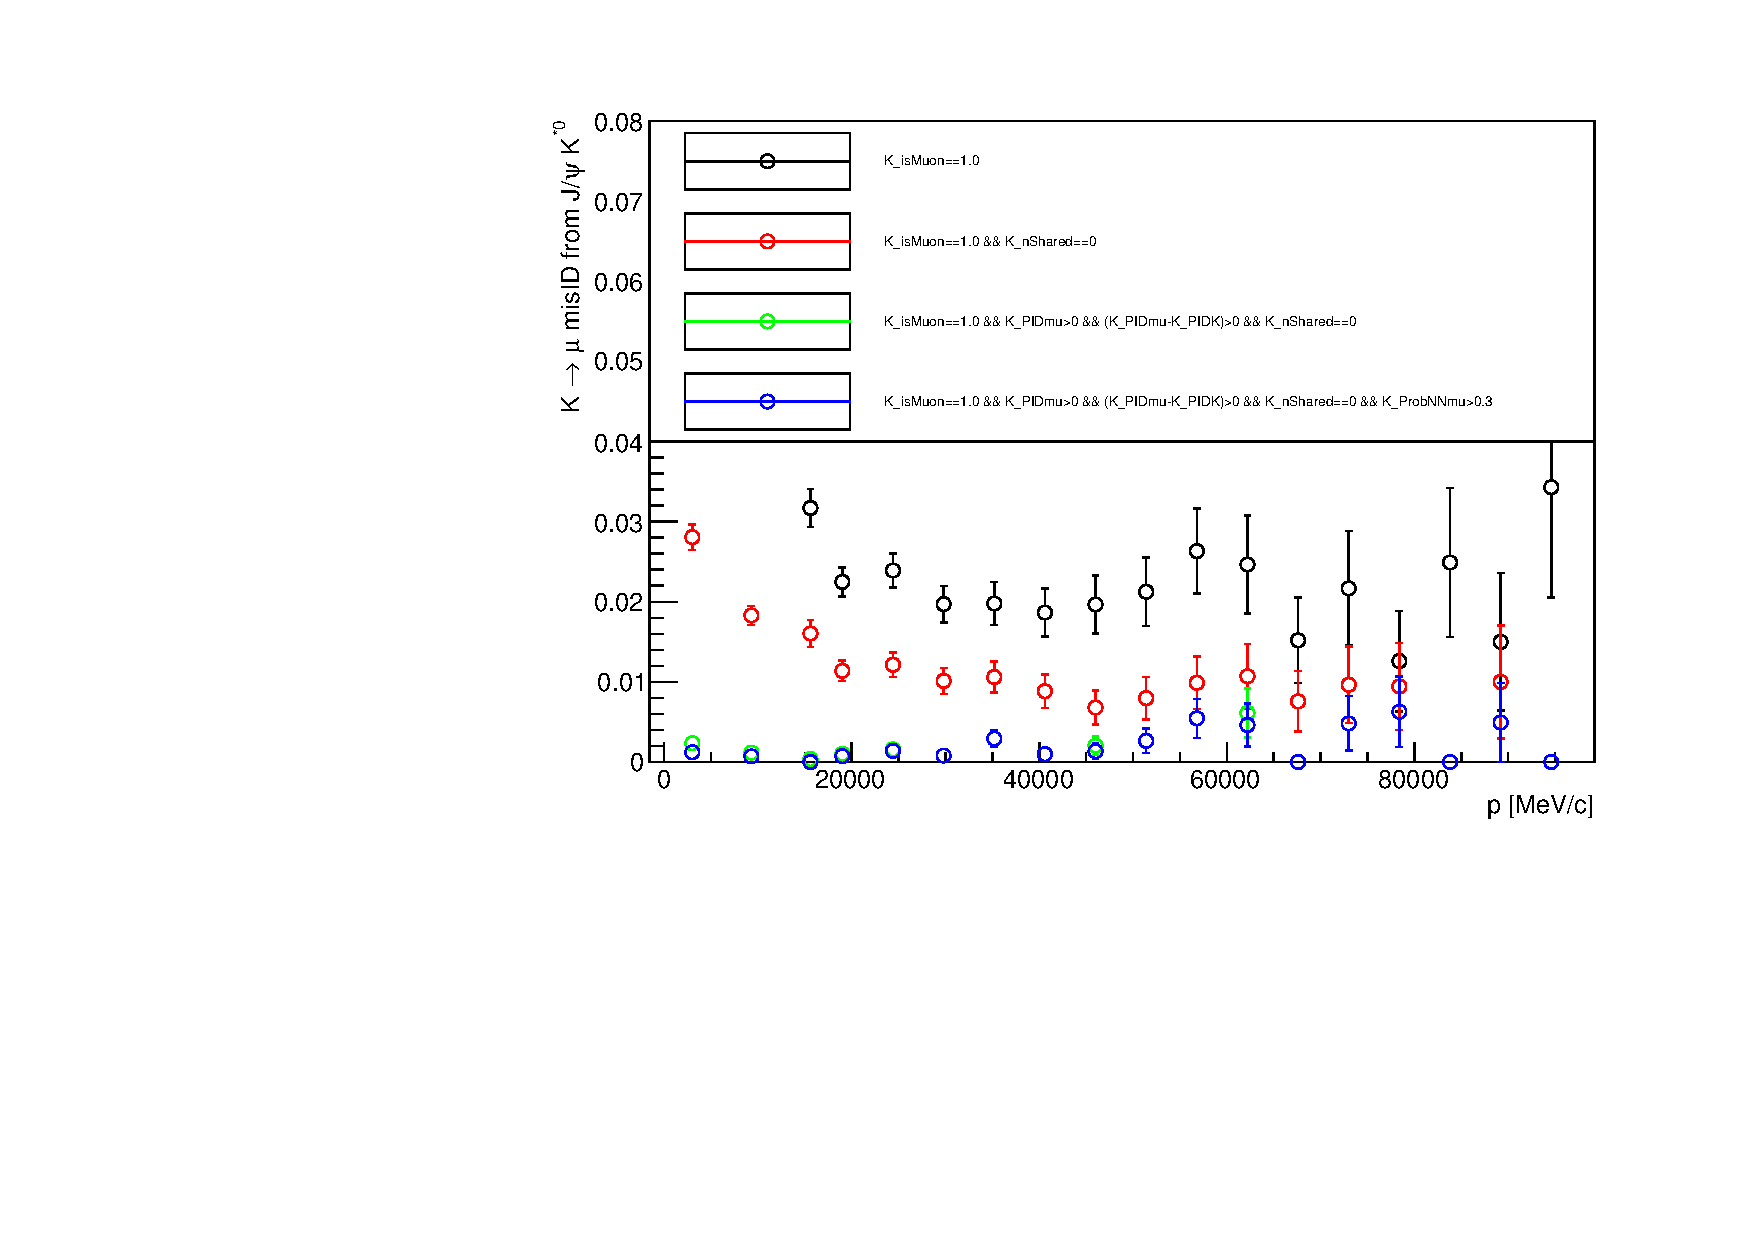
\includegraphics[width = 0.55\textwidth]{figs/trimuon/jpsikst/2012/Visualize_Weights_KaonMisid_2011_small.pdf}\put(-50,133){(a)}%
		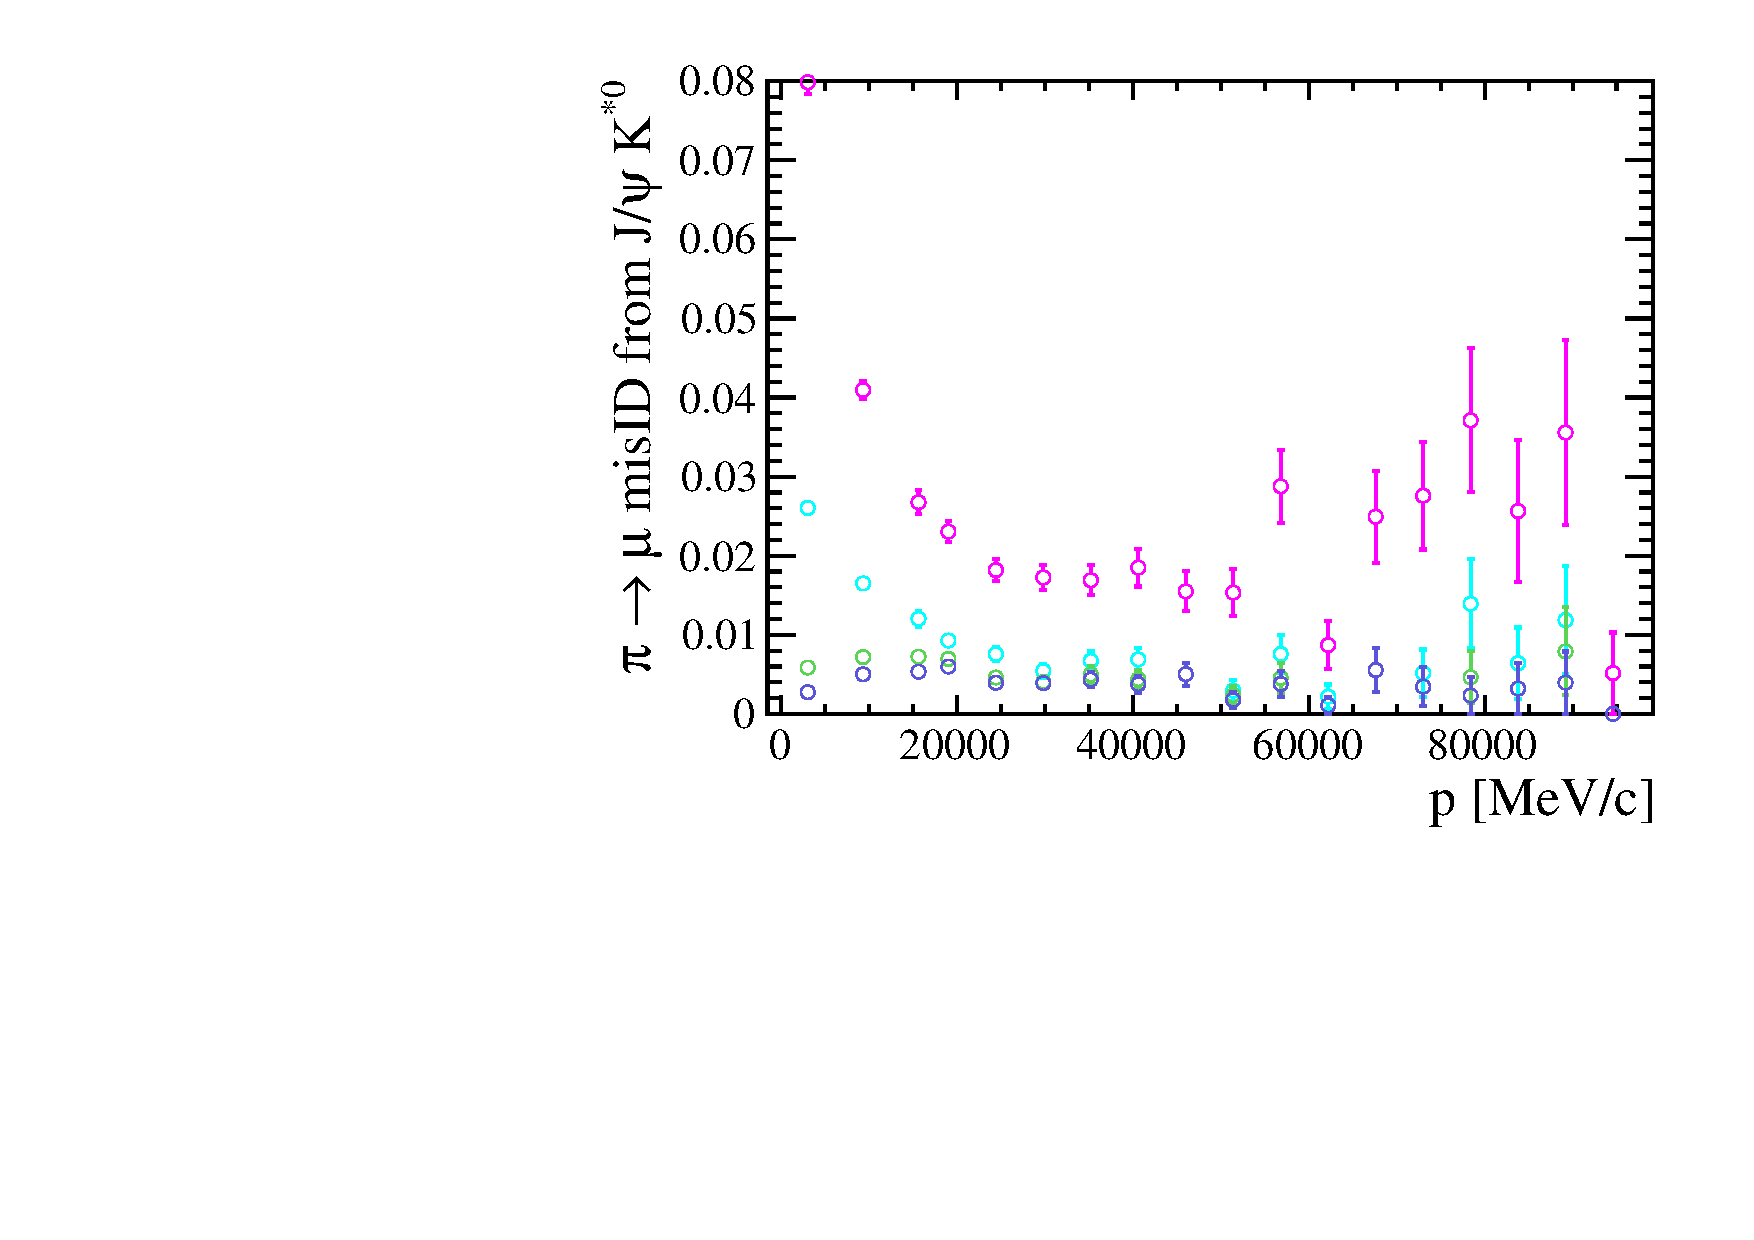
\includegraphics[width = 0.5\textwidth]{figs/trimuon/jpsikst/2012/Visualize_Weights_PionMisid_2012_small_thesis.pdf}\put(-50,133){(a)}
%		\newline
%		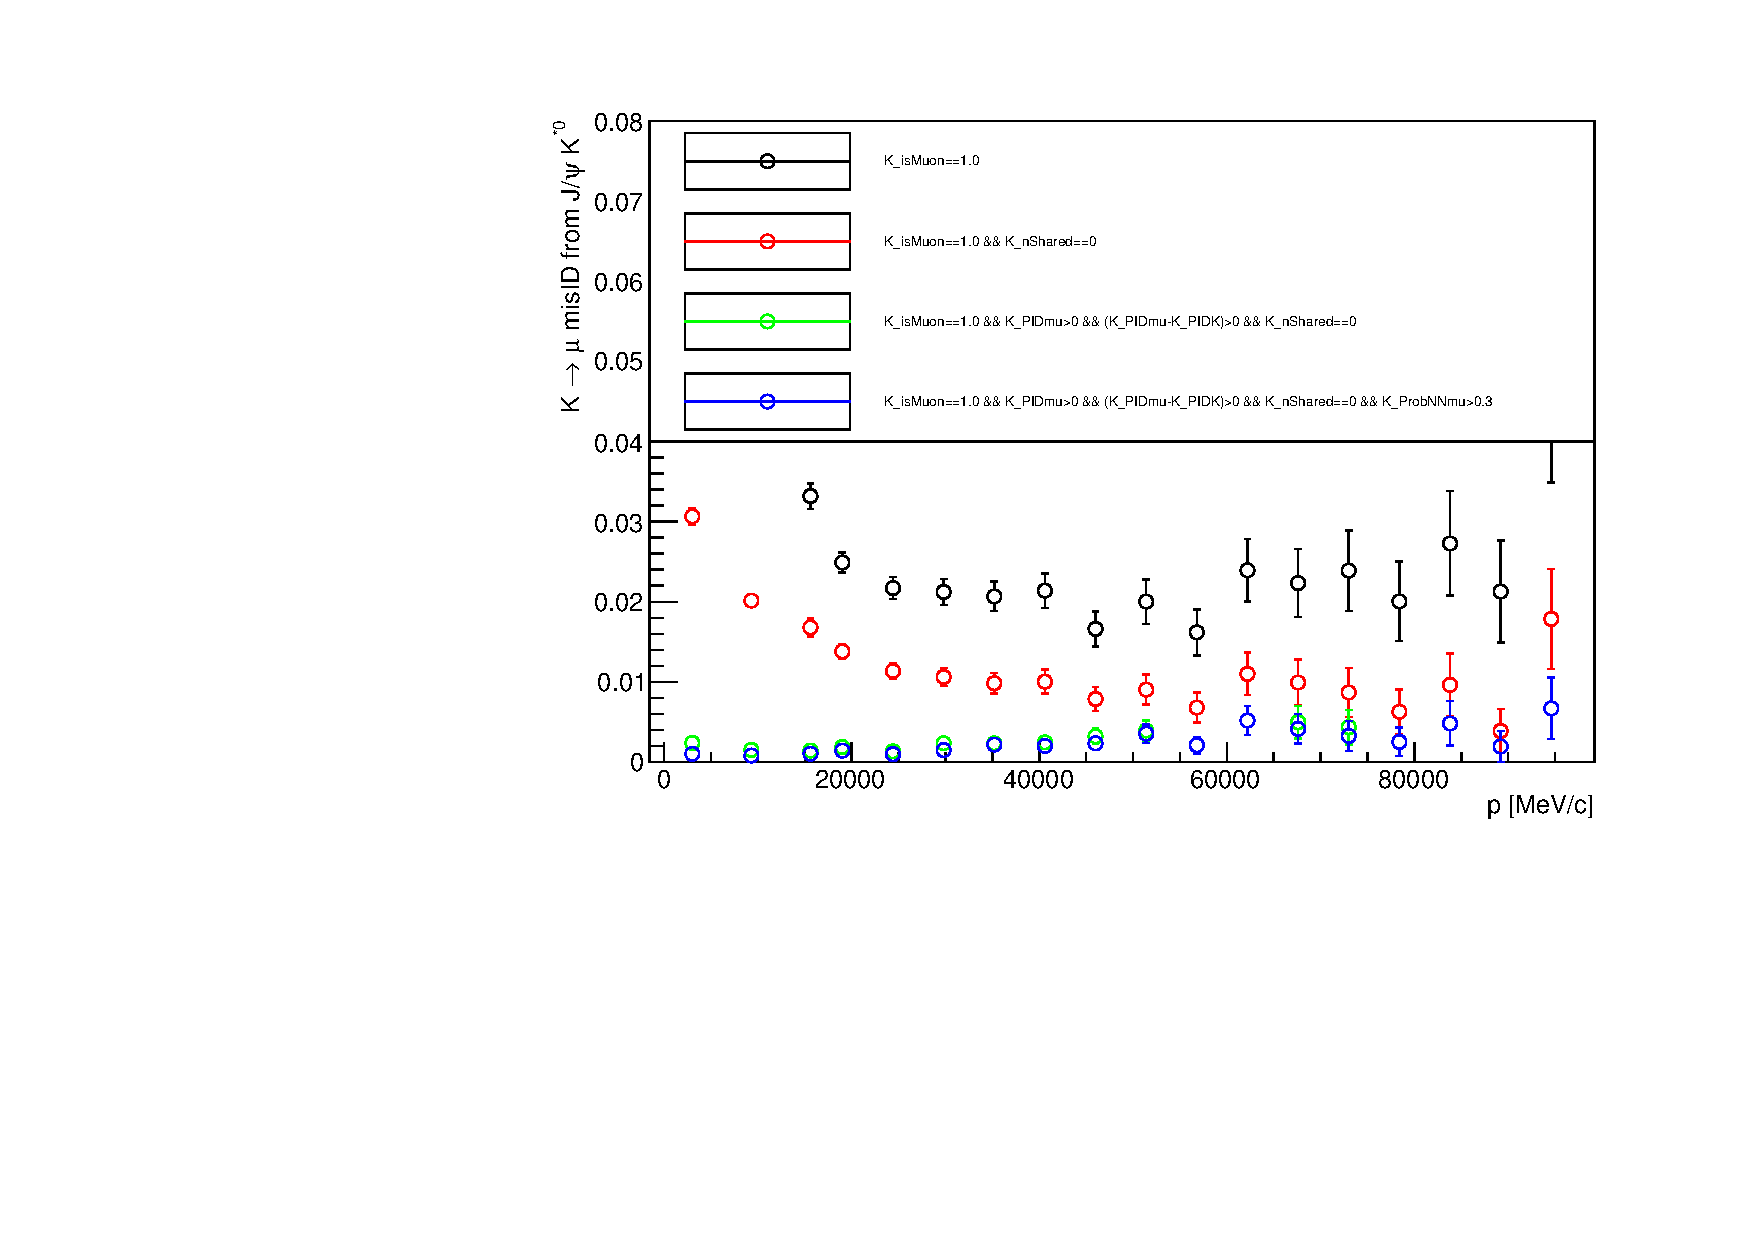
\includegraphics[width = 0.55\textwidth]{figs/trimuon/jpsikst/2012/Visualize_Weights_KaonMisid_small.pdf}\put(-50,133){(c)}%
		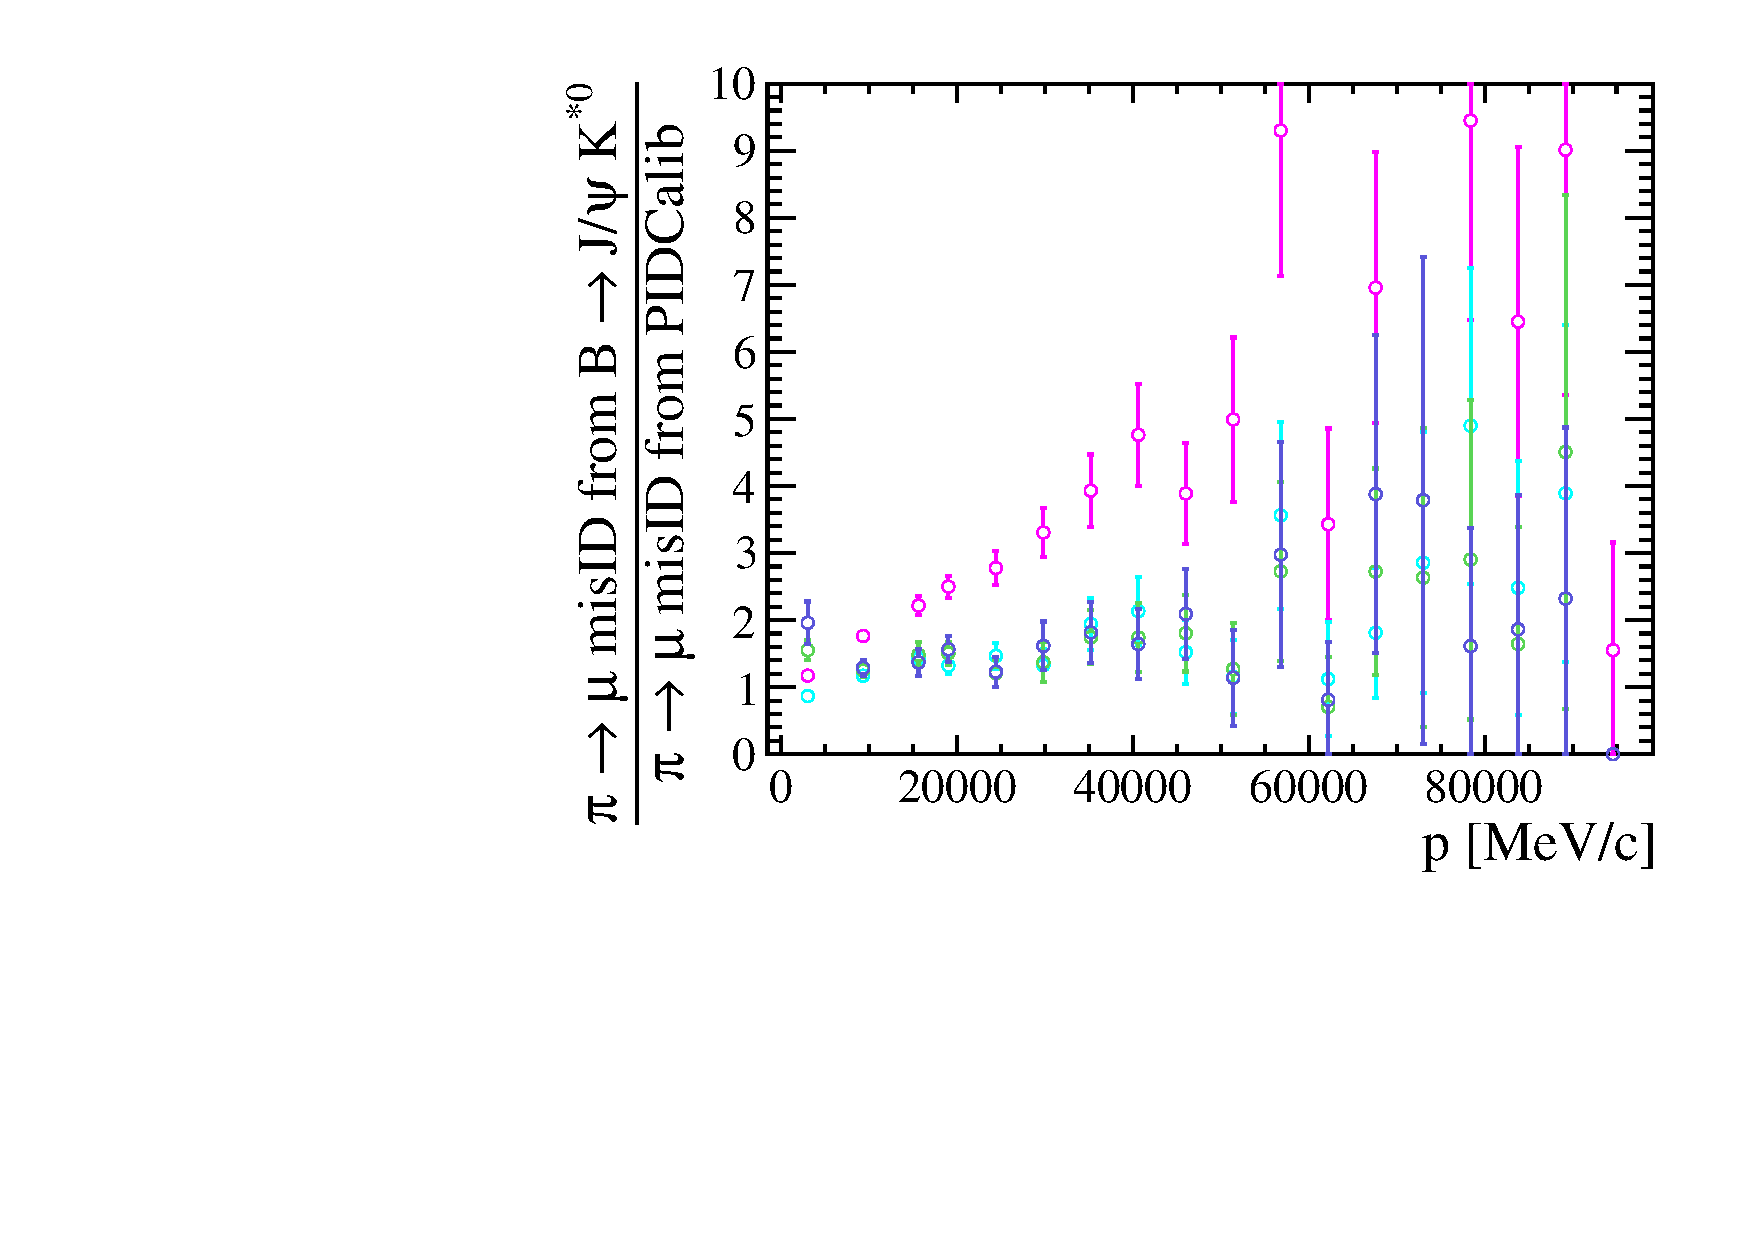
\includegraphics[width = 0.5\textwidth]{figs/trimuon/jpsikst/2012/Visualize_Ratios_PionMisid_small_thesis.pdf}\put(-50,133){(b)}
		\newline
%		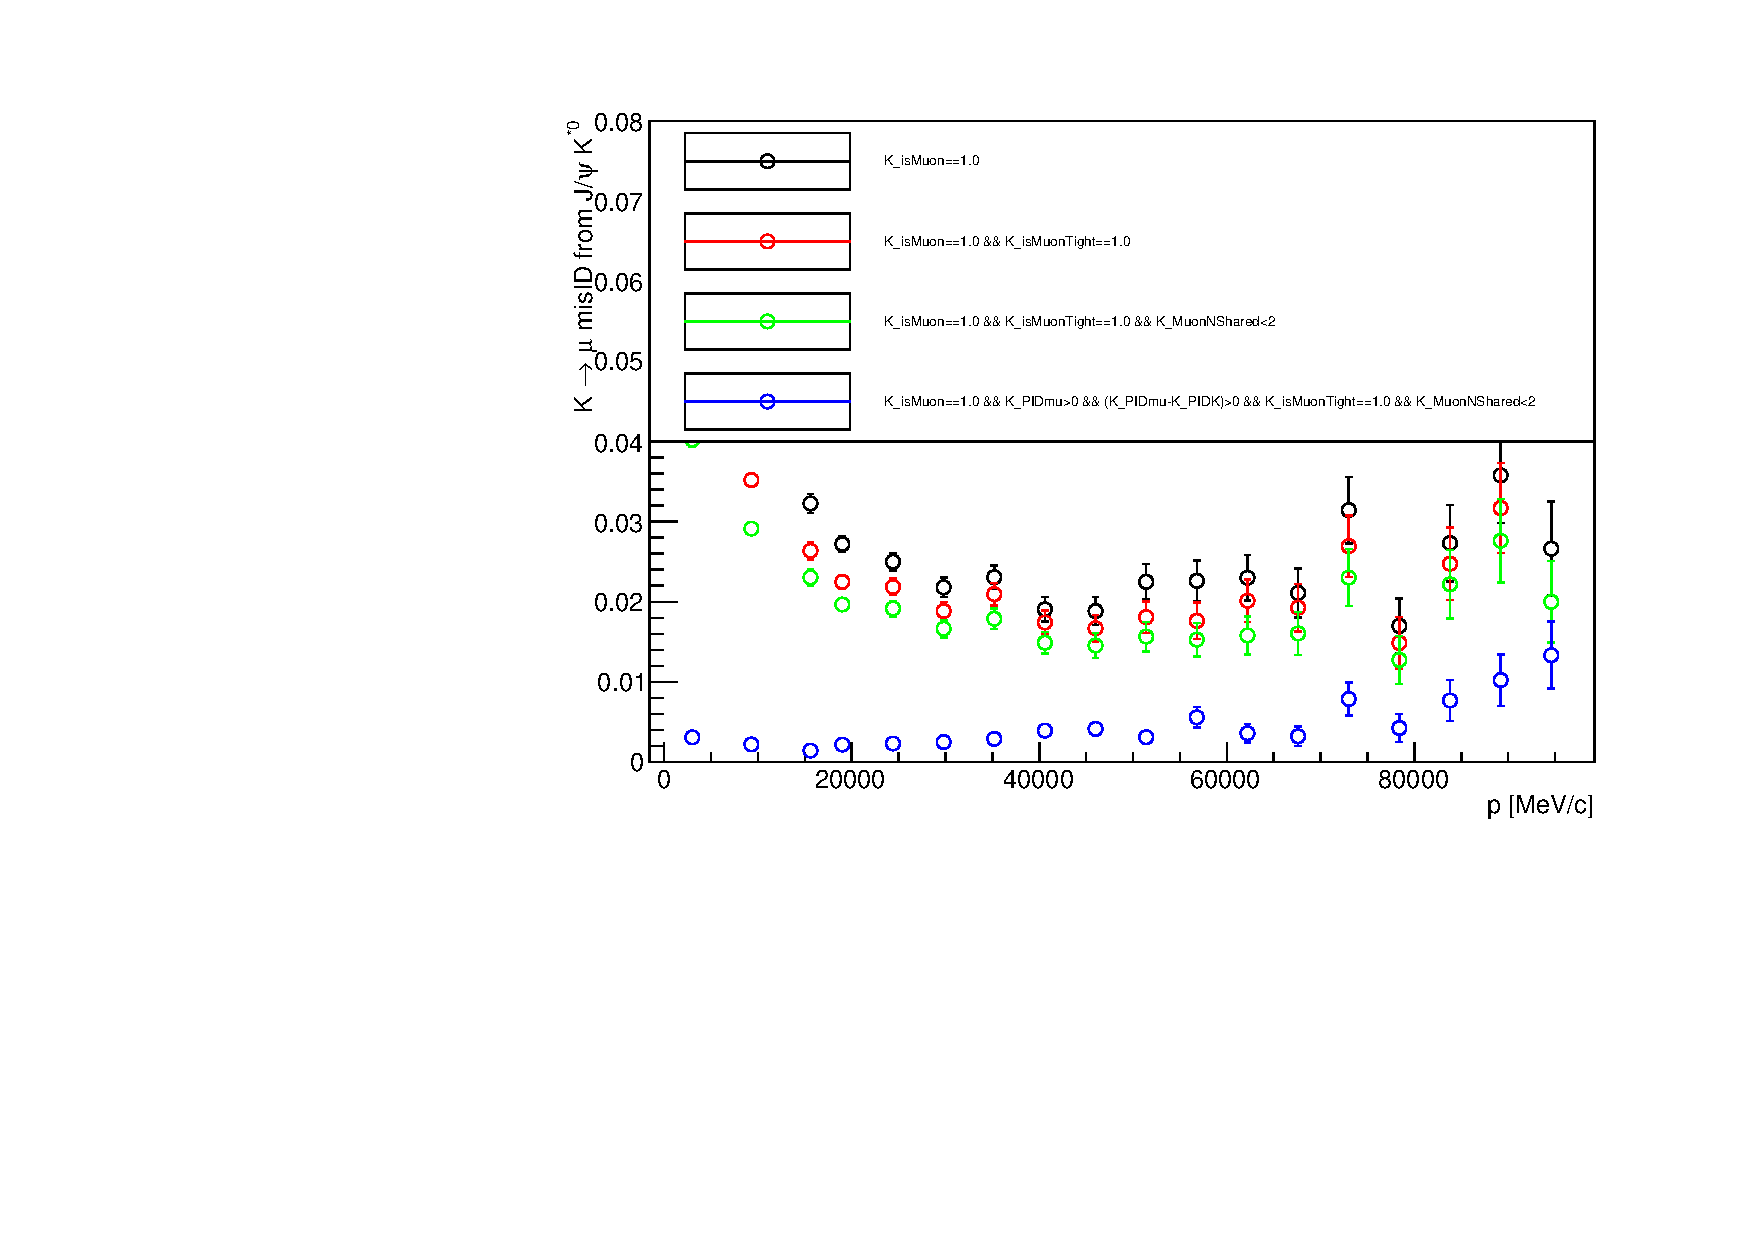
\includegraphics[width = 0.55\textwidth]{figs/trimuon/jpsikst/2012/Visualize_Weights_KaonMisid_2016_small.pdf}\put(-50,133){(e)}%
		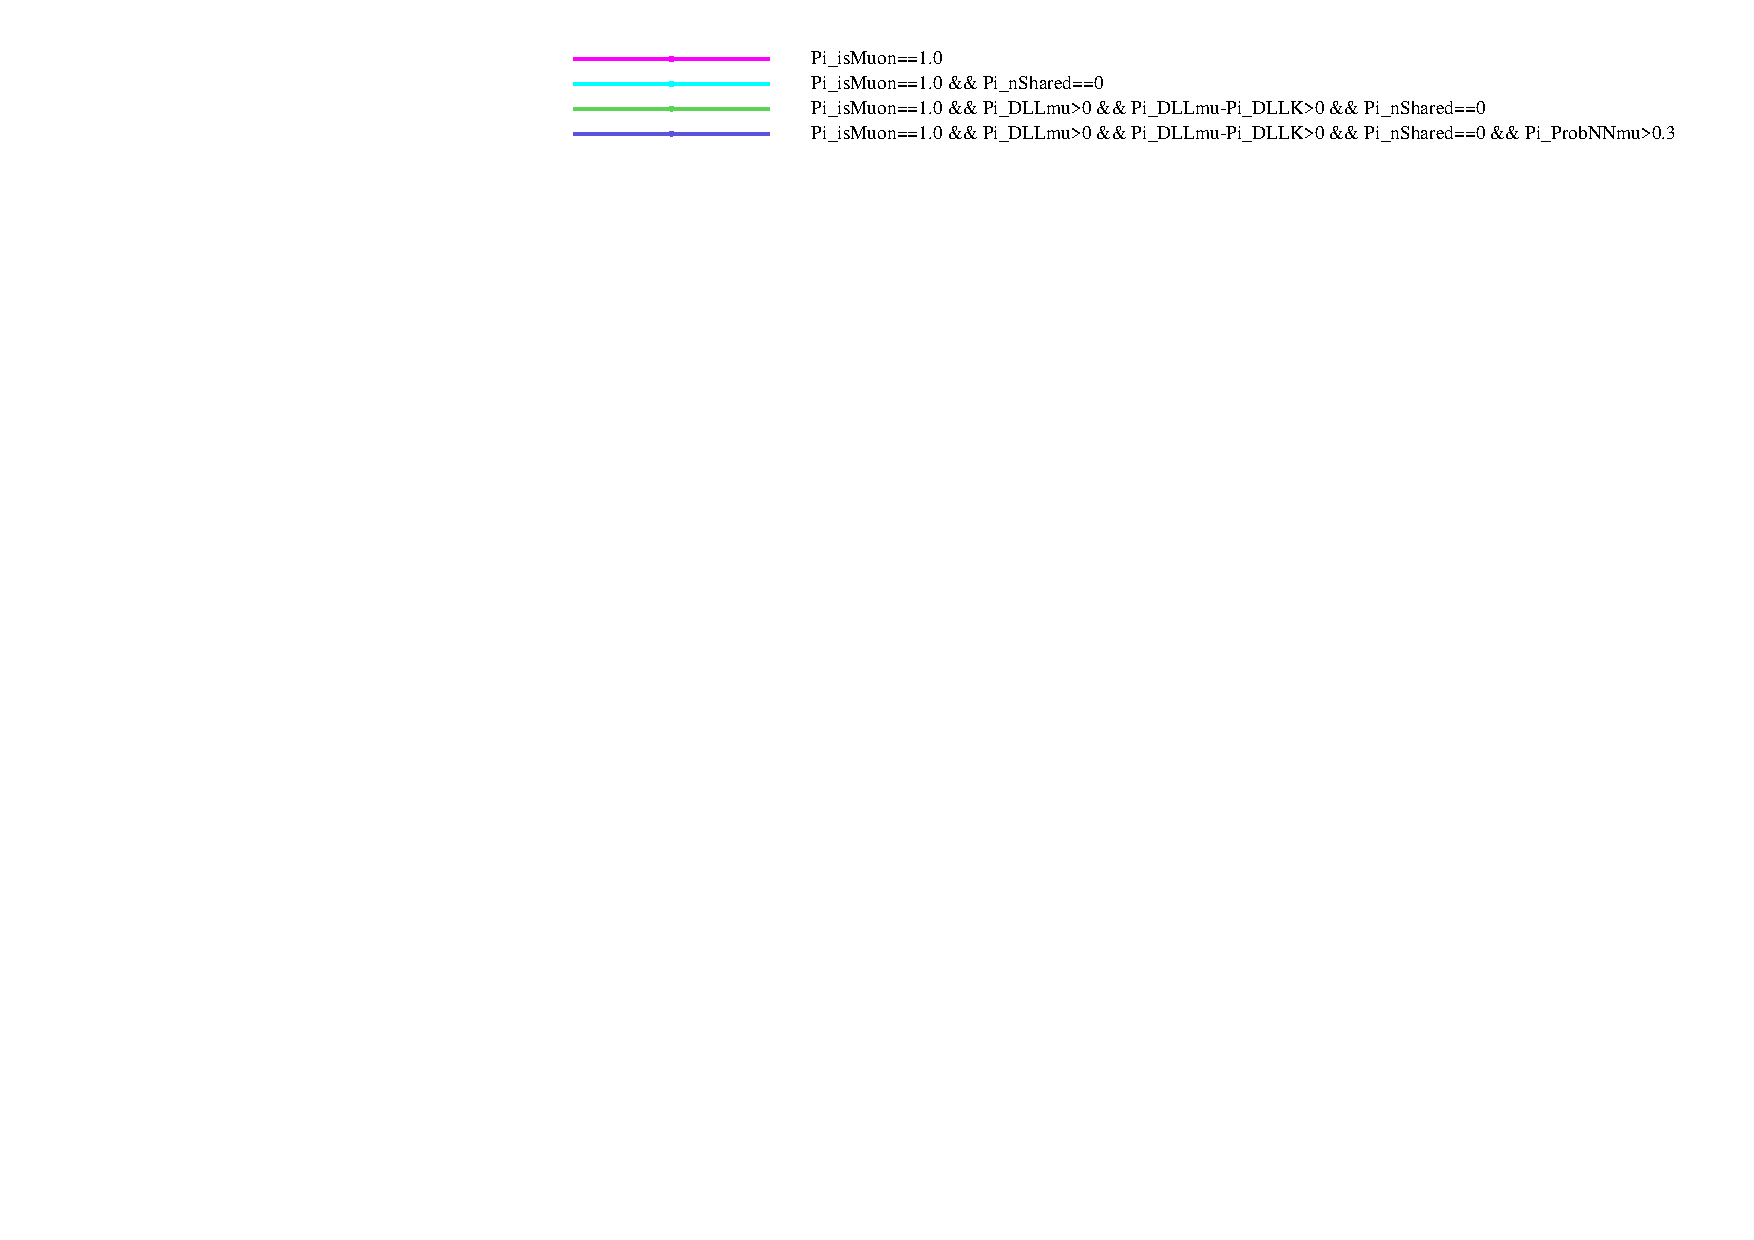
\includegraphics[width = 1.0\textwidth]{figs/trimuon/jpsikst/2012/Visualize_Weights_PionMisid_2012_small_thesis_legend.pdf}
		\caption{(a) $\pi \rightarrow \mu$ misID probabibility for different PID requirements obtained using $B^{0} \rightarrow J/\psi(\rightarrow \mu^{+} \mu^{-}) K^{*} (\rightarrow {K^{+} \pi^{-}} )$ for 2012 data. (b) This is compared to the standard \texttt{PIDCalib} $D^{*+}(\rightarrow D^{0}(\rightarrow K^{+} \pi^{-}) \pi^{+})$ sample. }
		\label{fig:JpsiKnew}
\end{figure}

%Using the \textit{sWeight} method, misID rates for kaons and pions can be obtained. Two control samples that are analysed are $D^{*+}(\rightarrow D^{0}(\rightarrow \underline{K^{+} \pi^{-}}) \pi^{+})$ events and $B^{0} \rightarrow J/\psi(\rightarrow \mu^{+} \mu^{-}) K^{*}$ events.
%In general the agreement is good in the low momentum regions between the two samples as shown in ~\autoref{fig:JpsiKnew}. These pions are softer and hence they will spread out more in the magnetic field, causing less interference with other two real muons in decay. However, in high momentum region, the pion will follow a path through the muon system that is more similar to the path of the muon of the same charge in the $B^{0} \rightarrow J/\psi(\rightarrow \mu^{+} \mu^{-}) K^{*}$ decay. The influence of other two real muons in high momenta region will lead to bigger disagreement as these two real muons leave hits in the muon chambers close to the collimated pion track, making the rate of \texttt{IsMuon==1.0} (pink) is higher. 

This disagreement is decreased by requiring \texttt{nShared==0.0} (blue), as having two other collimated muons to share hits will be more likely. The effect of other \gls{PID} variables can also be seen, but it is harder to interpret as these depend on several variables.

Even though this disagreement is decreased, for the high momenta region $\pi \rightarrow \mu$ ~\autoref{fig:JpsiKnew} and $K \rightarrow \mu$~\autoref{fig:JpsiKaonnew} rate is 2 to 3 times higher with additional two real muon tracks. Such disagreement is significant and if the misID rates from the standard control samples were to be used to be parametrically applied on samples to estimate the misID background, there would be an underestimate the misID component by the same factor.

In conclusion, it was shown that the standard misID samples are not good proxies for estimating the misID probabilities as there is interference from two other muons in the event. Instead, the misID probabilities that are used in calculations for the misID background for \Bmumumu are obtained from \textit{Sweighted} $B^{0} \rightarrow J/\psi(\rightarrow \mu^{+} \mu^{-}) K^{*}$. Remaining effects of taking this sample for calibration are considered as a systematic uncertainty, with more details in~\autoref{misidfitstrat}.



\begin{figure}[h!]
\center
%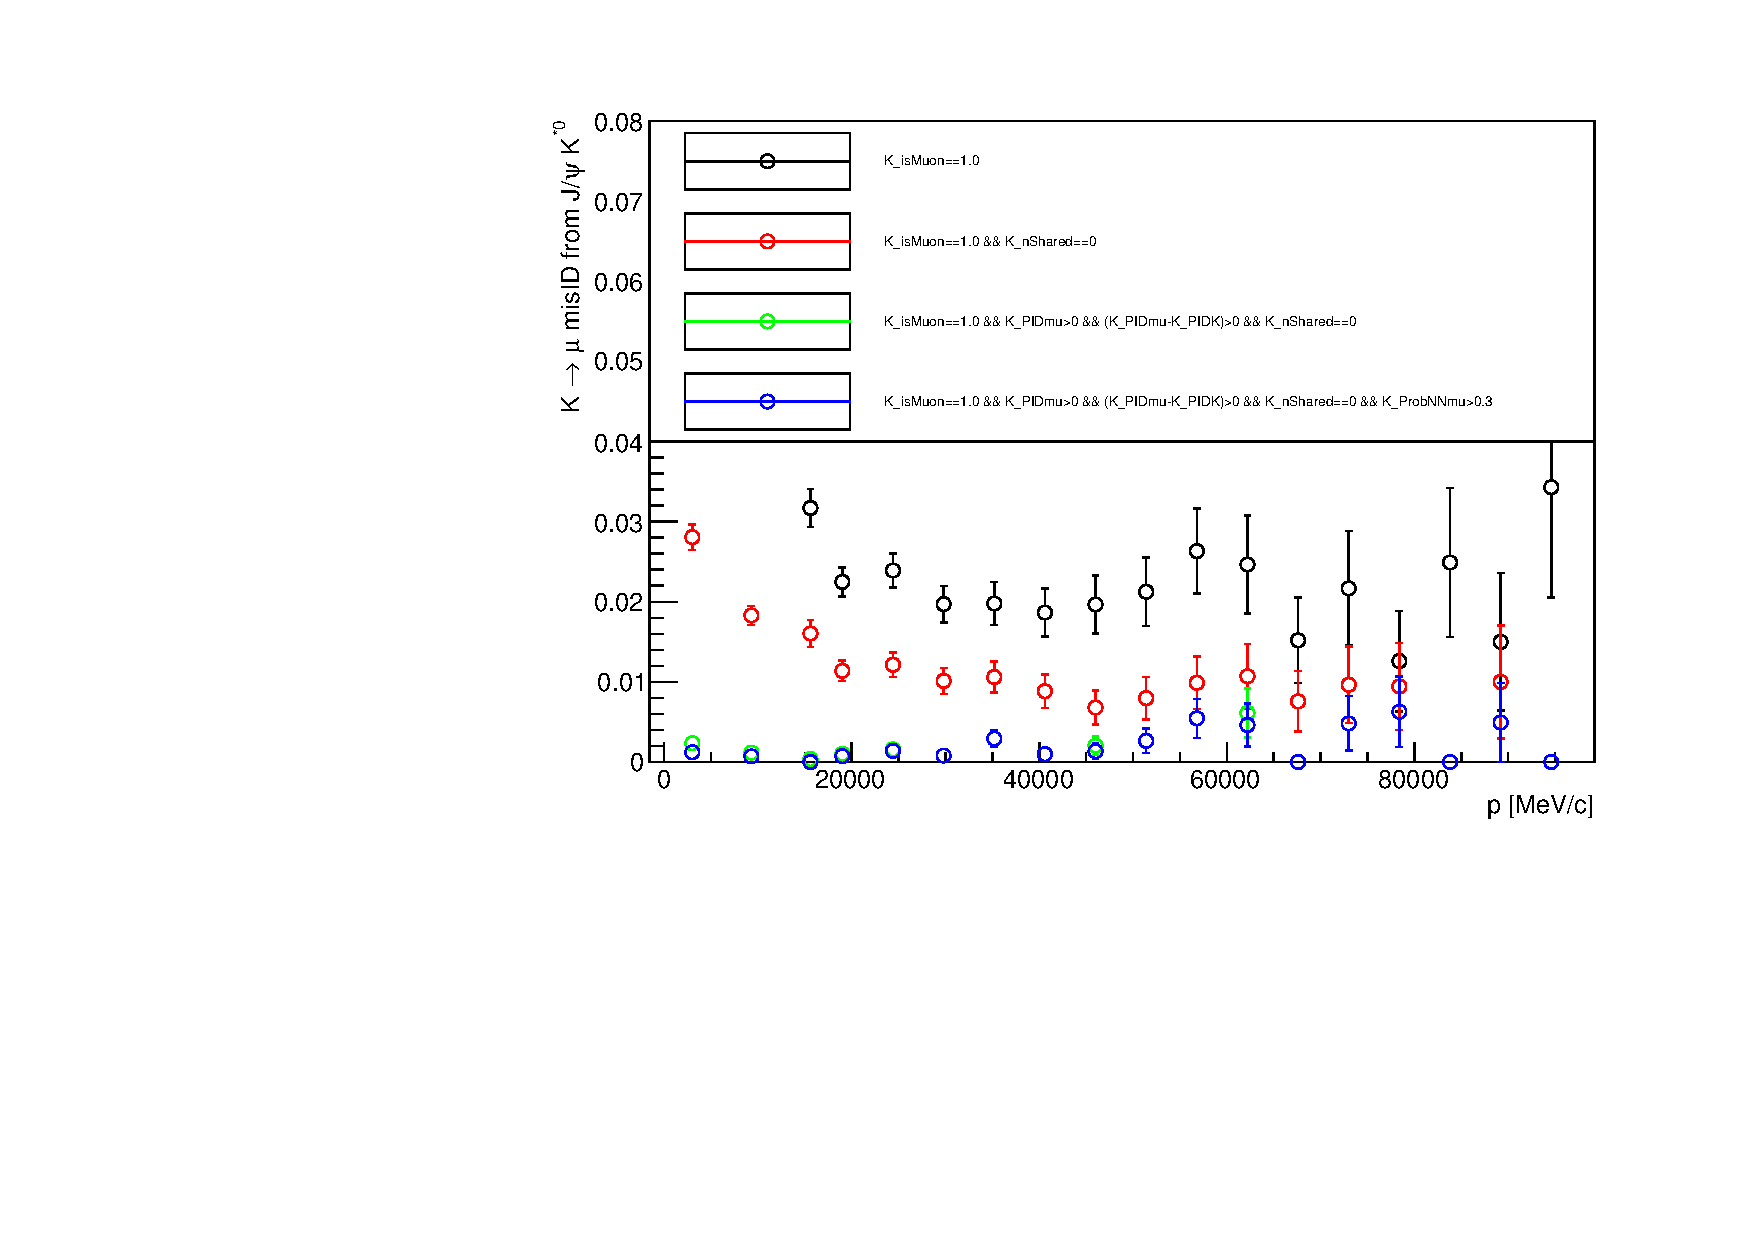
\includegraphics[width = 0.55\textwidth]{figs/trimuon/jpsikst/2012/Visualize_Weights_KaonMisid_2011_small.pdf}\put(-50,133){(a)}%
		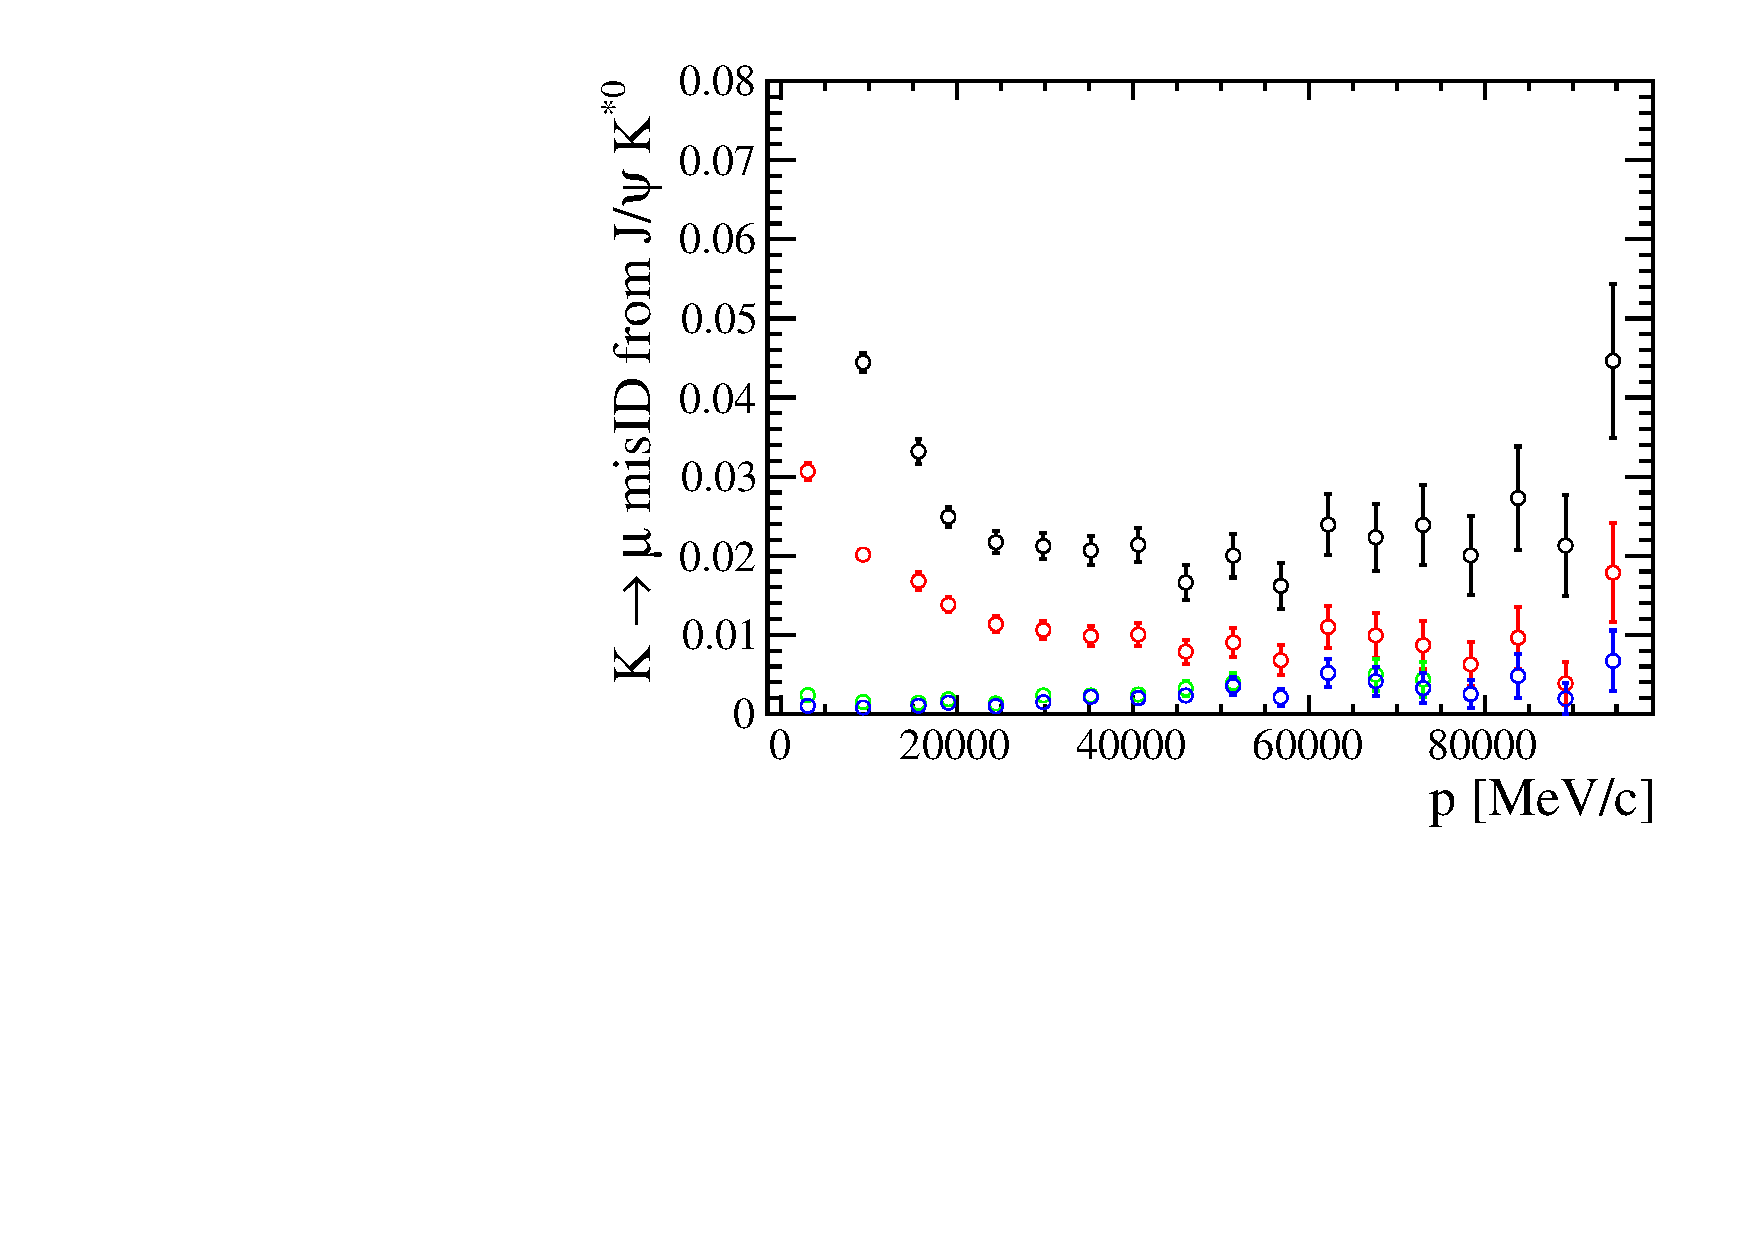
\includegraphics[width = 0.5\textwidth]{figs/trimuon/jpsikst/2012/Visualize_Weights_KaonMisid_2012_small_thesis.pdf}\put(-50,133){(a)}
%		\newline
%		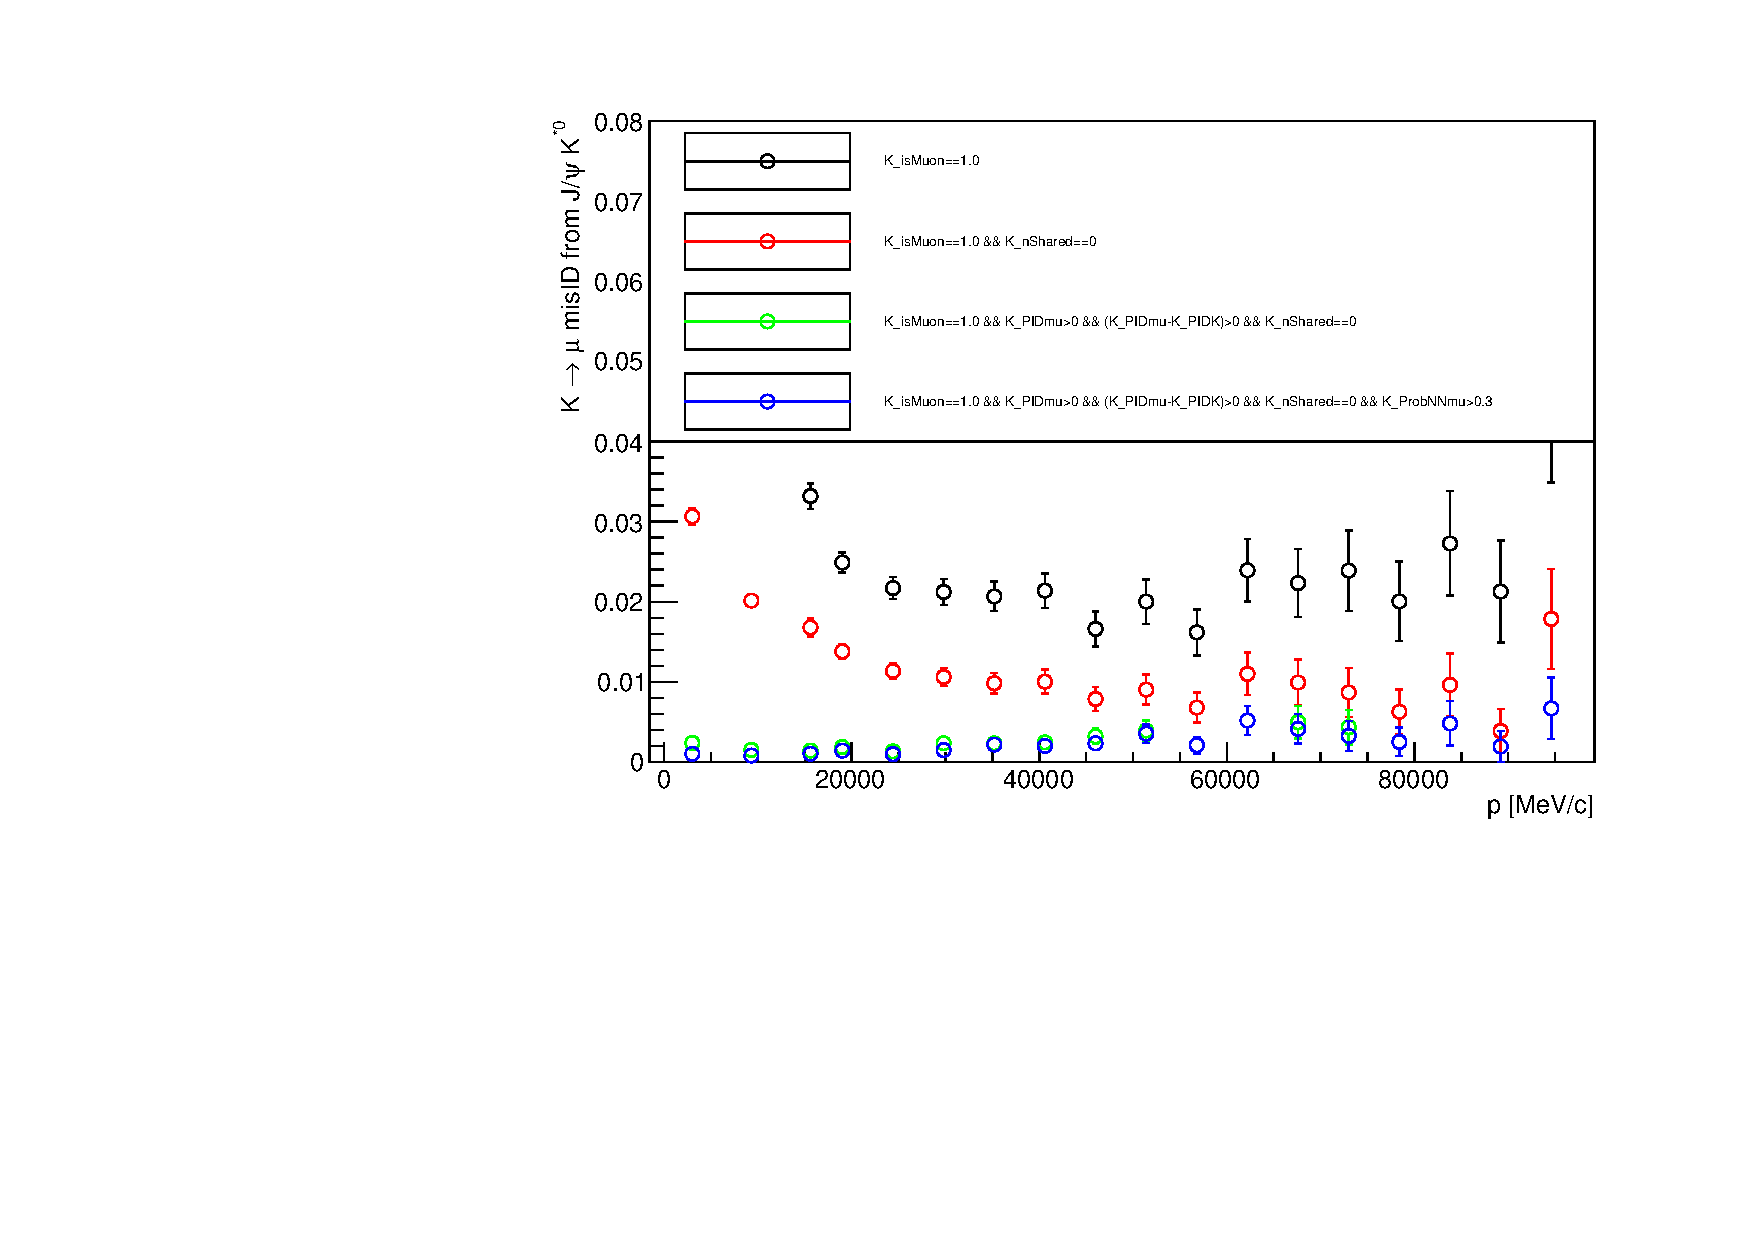
\includegraphics[width = 0.55\textwidth]{figs/trimuon/jpsikst/2012/Visualize_Weights_KaonMisid_small.pdf}\put(-50,133){(c)}%
		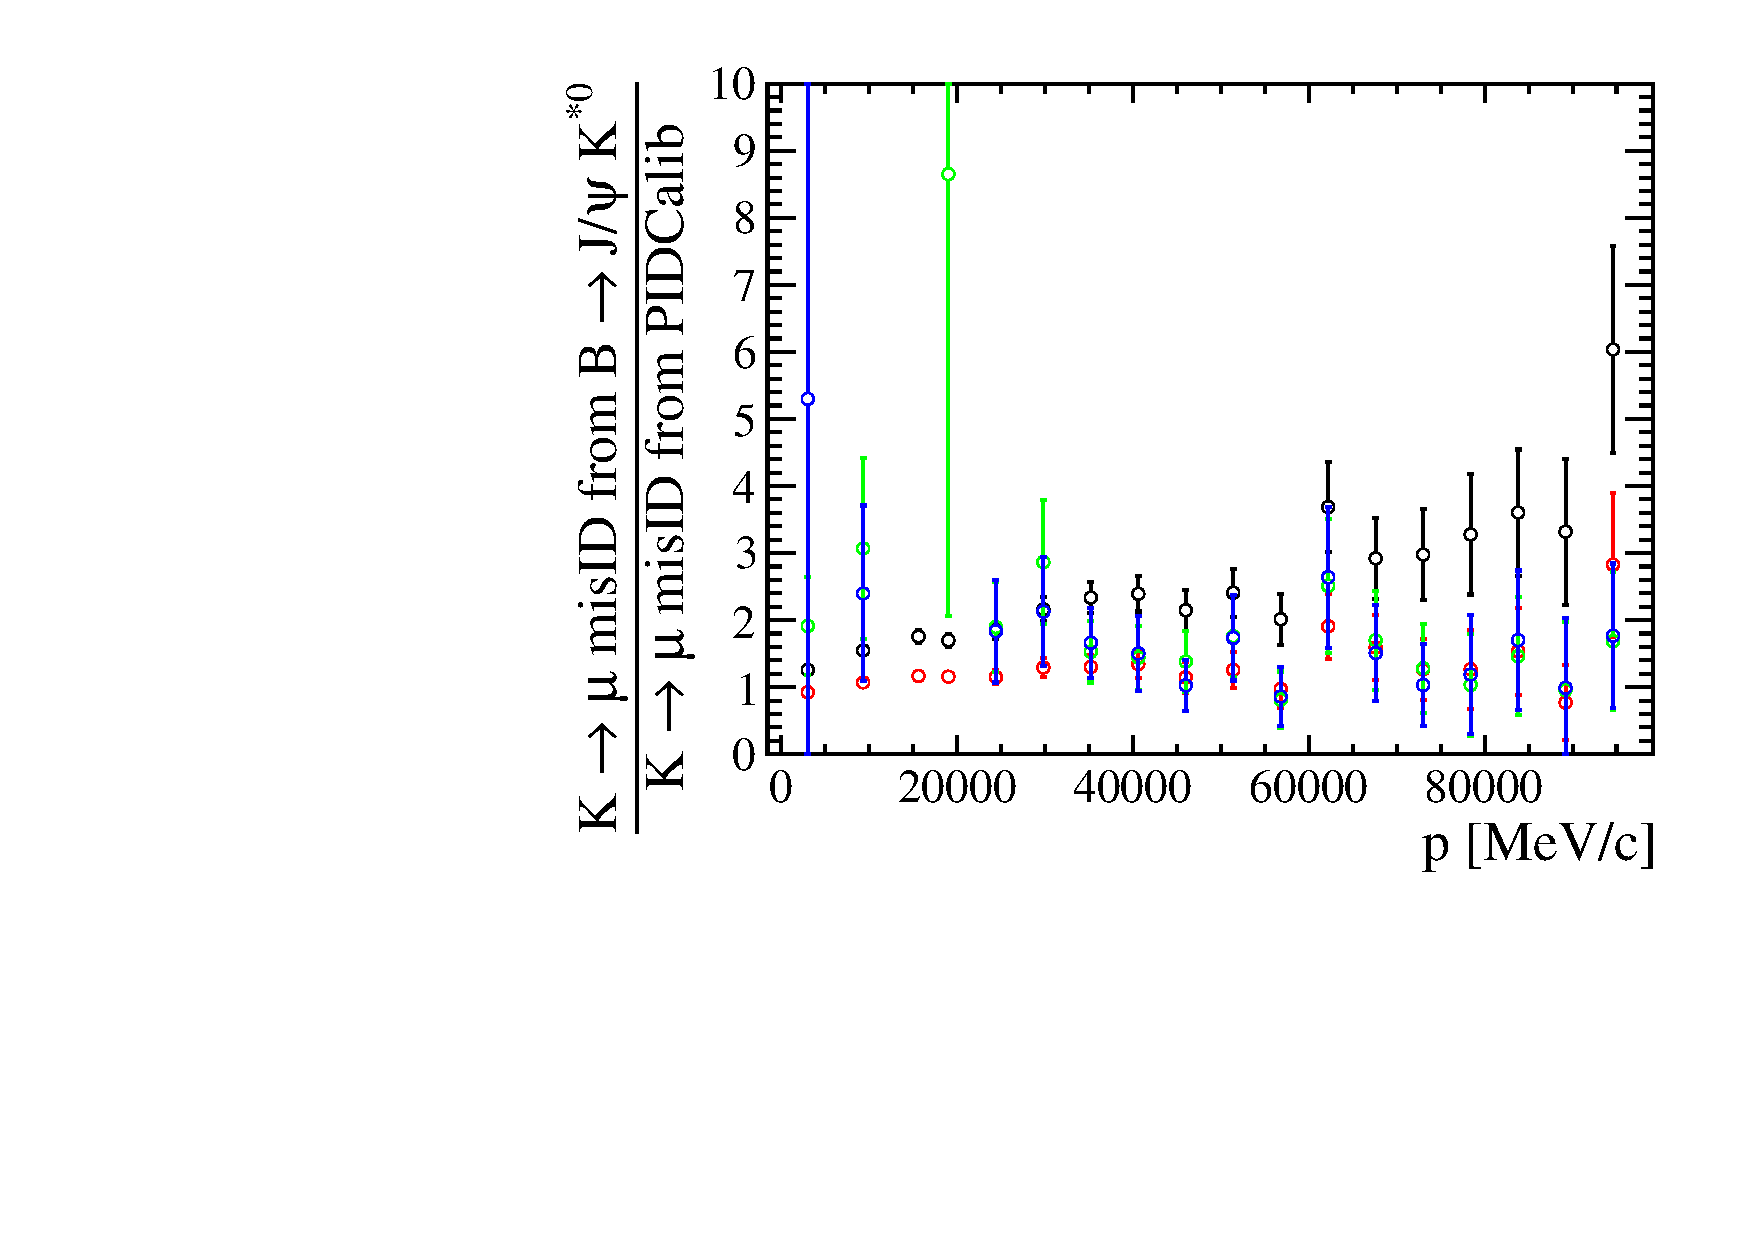
\includegraphics[width = 0.5\textwidth]{figs/trimuon/jpsikst/2012/Visualize_Ratios_KaonMisid_small_thesis.pdf}\put(-50,133){(b)}
		\newline
%		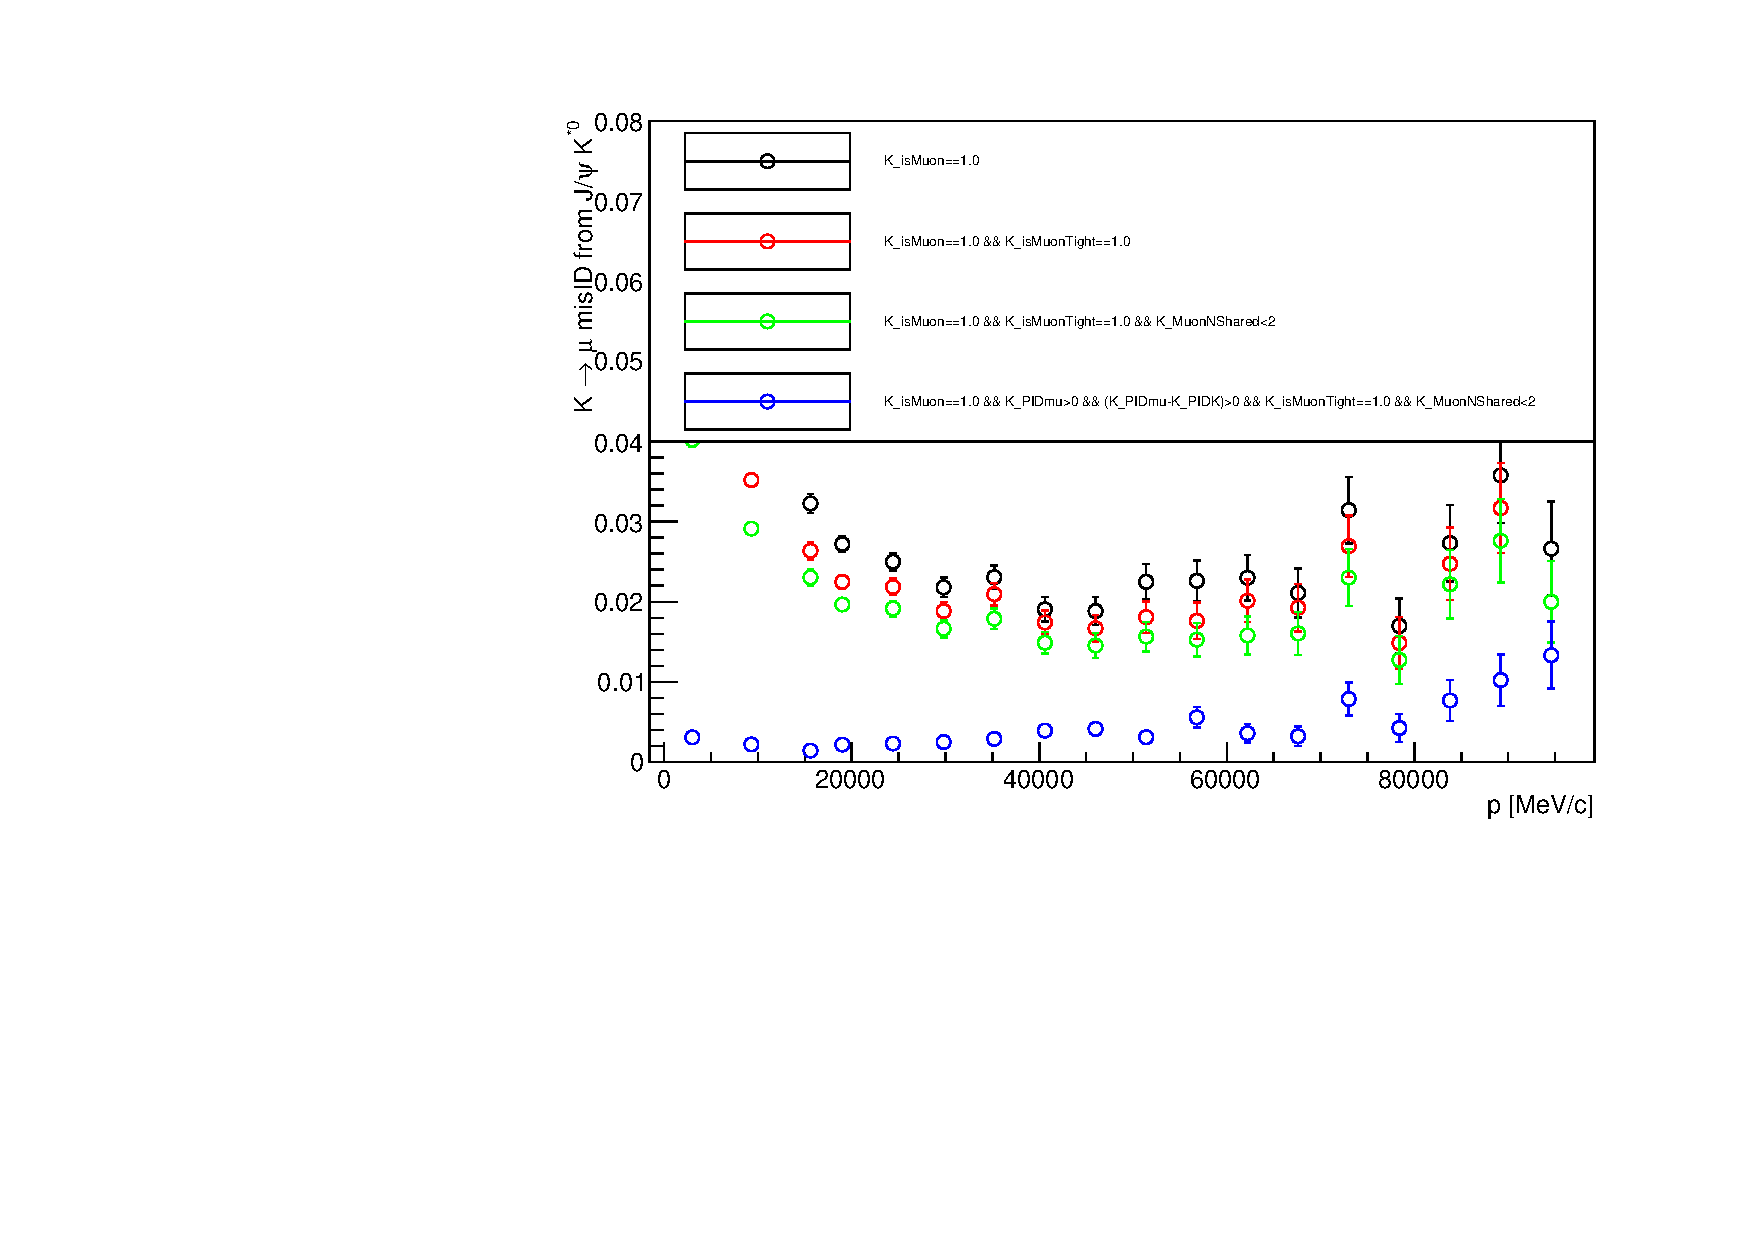
\includegraphics[width = 0.55\textwidth]{figs/trimuon/jpsikst/2012/Visualize_Weights_KaonMisid_2016_small.pdf}\put(-50,133){(e)}%
		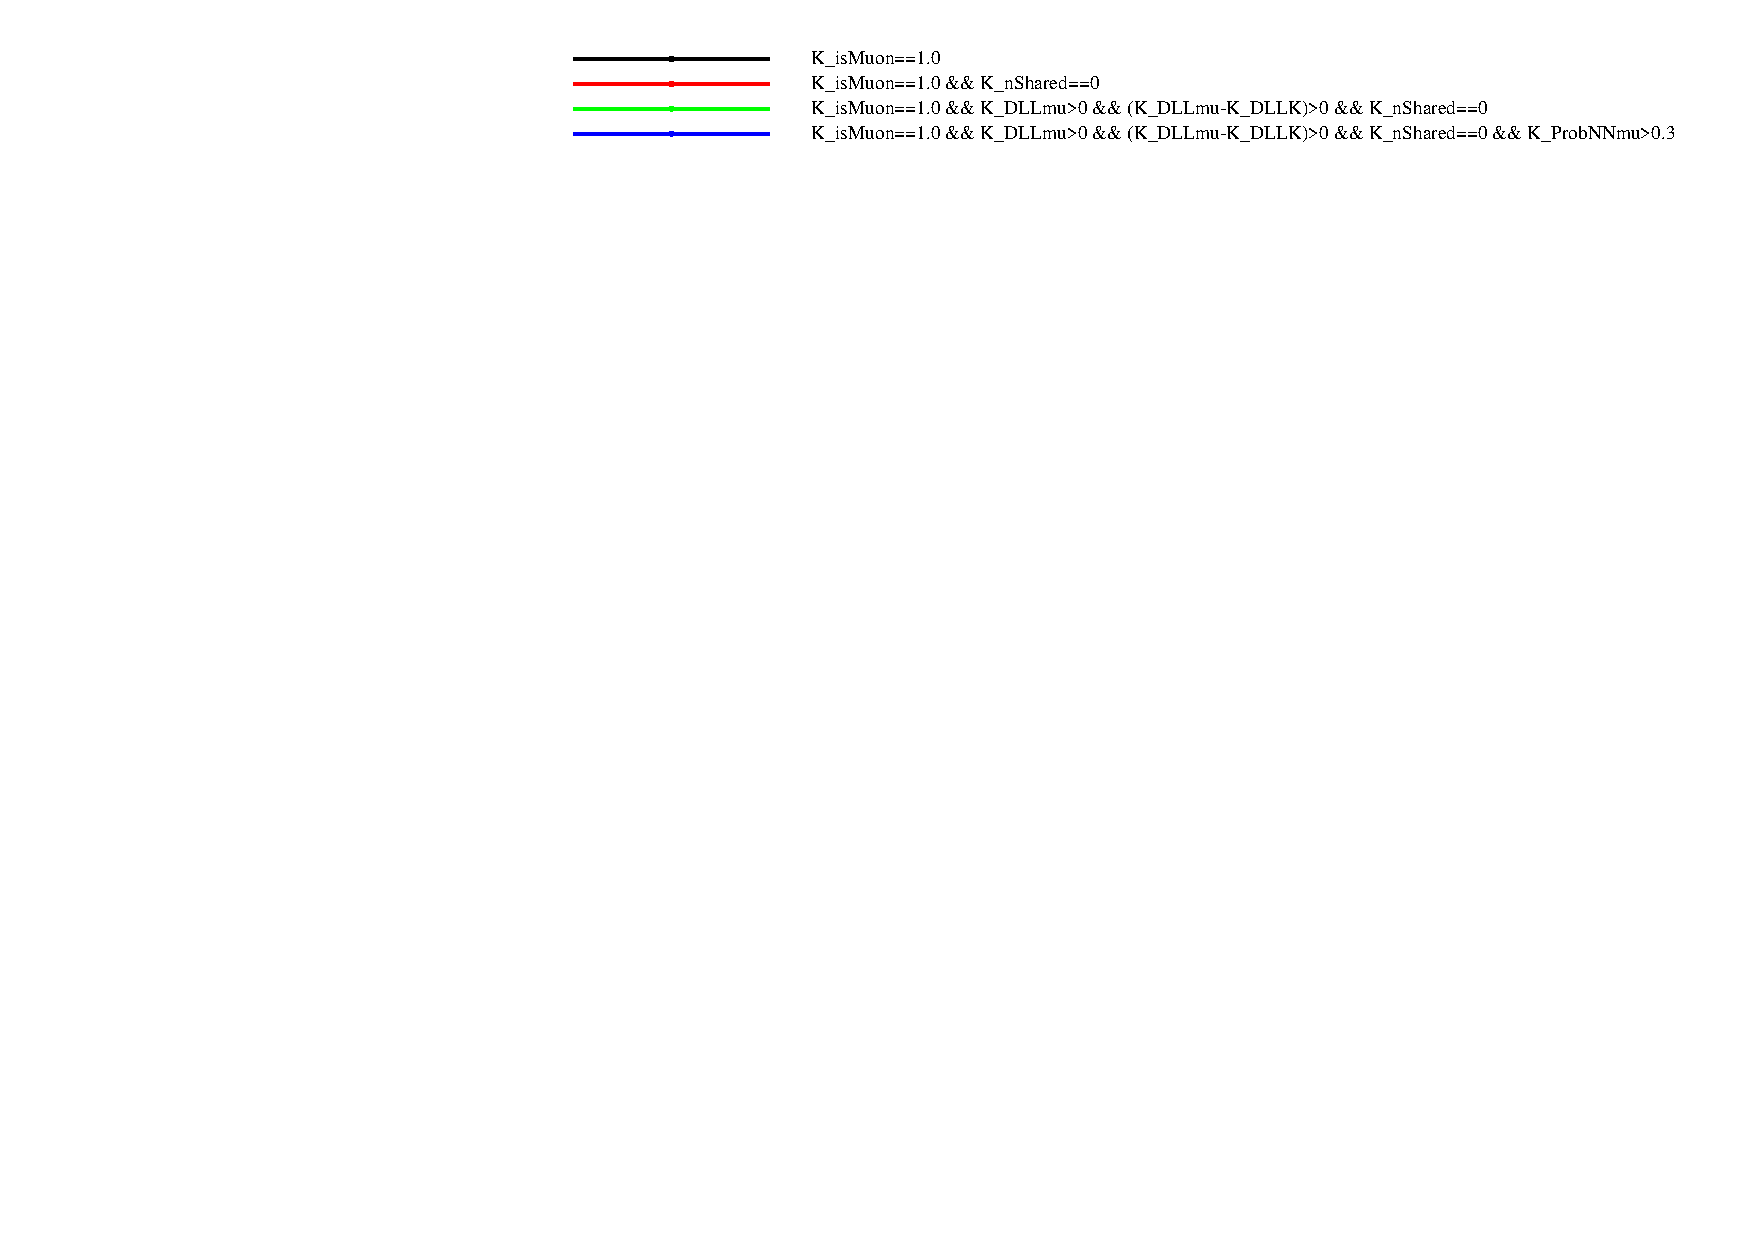
\includegraphics[width = 1.0\textwidth]{figs/trimuon/jpsikst/2012/Visualize_Weights_KaonMisid_2012_small_thesis_legend.pdf}
		\caption{(a) $K \rightarrow \mu$ misID probabibility for different PID requirements obtained using $B^{0} \rightarrow J/\psi(\rightarrow \mu^{+} \mu^{-}) K^{*} (\rightarrow {K^{+} \pi^{-}} )$ for 2012 data. (b) This is compared to the standard \texttt{PIDCalib} $D^{*+}(\rightarrow D^{0}(\rightarrow K^{+} \pi^{-}) \pi^{+})$ sample. }
		\label{fig:JpsiKaonnew}
\end{figure}

Due to the different \gls{PID} definitions of \texttt{nShared} between Run \Rn{1} and \Rn{2}, different \gls{PID} requirement are tested.  Results for $\pi \rightarrow \mu$ and $K \rightarrow \mu$ are summarized in~\autoref{fig:JpsiPionnew2016} and
~\autoref{fig:JpsiKaonnew2016}. The misID probabilities in 2016 for also show the same momentum dependent trend as in 2012. 



\begin{figure}[h!]
\center
%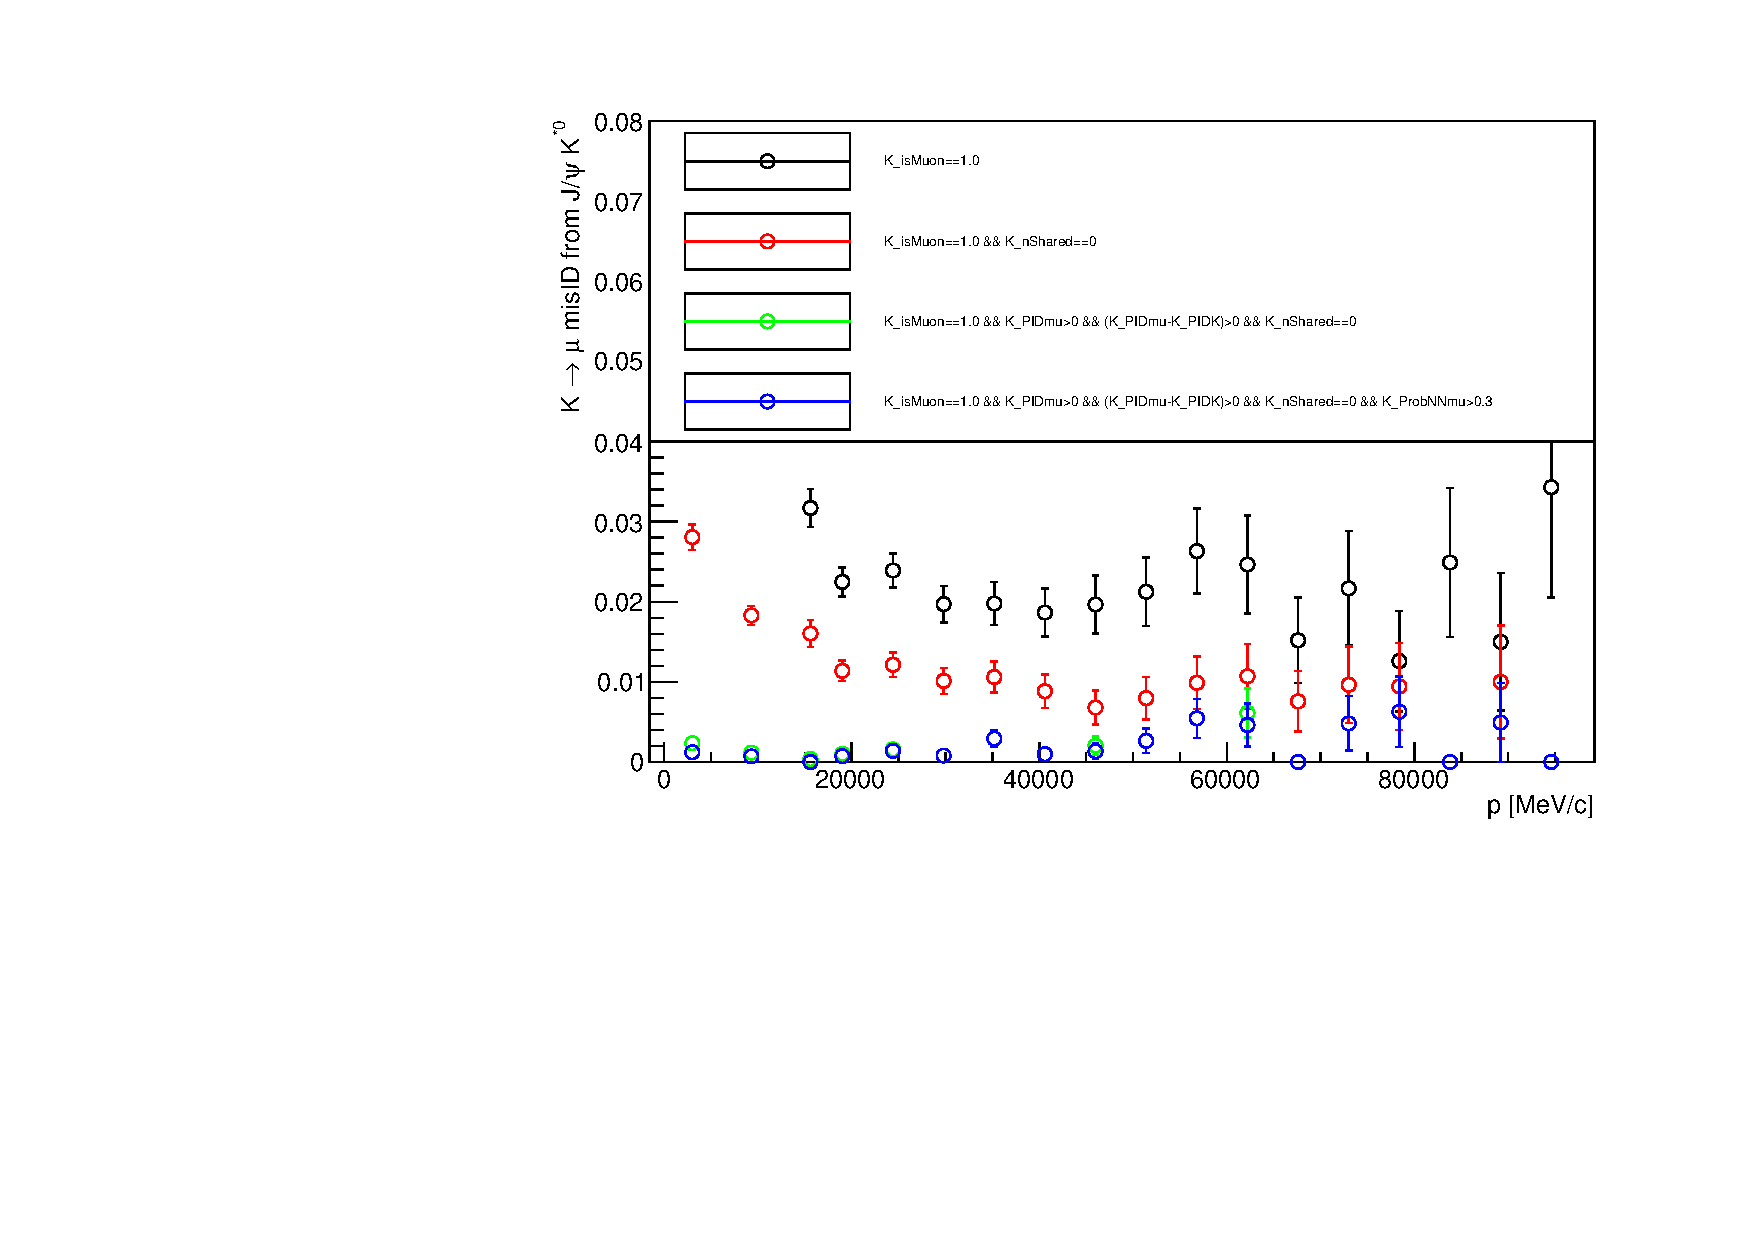
\includegraphics[width = 0.55\textwidth]{figs/trimuon/jpsikst/2012/Visualize_Weights_KaonMisid_2011_small.pdf}\put(-50,133){(a)}%
		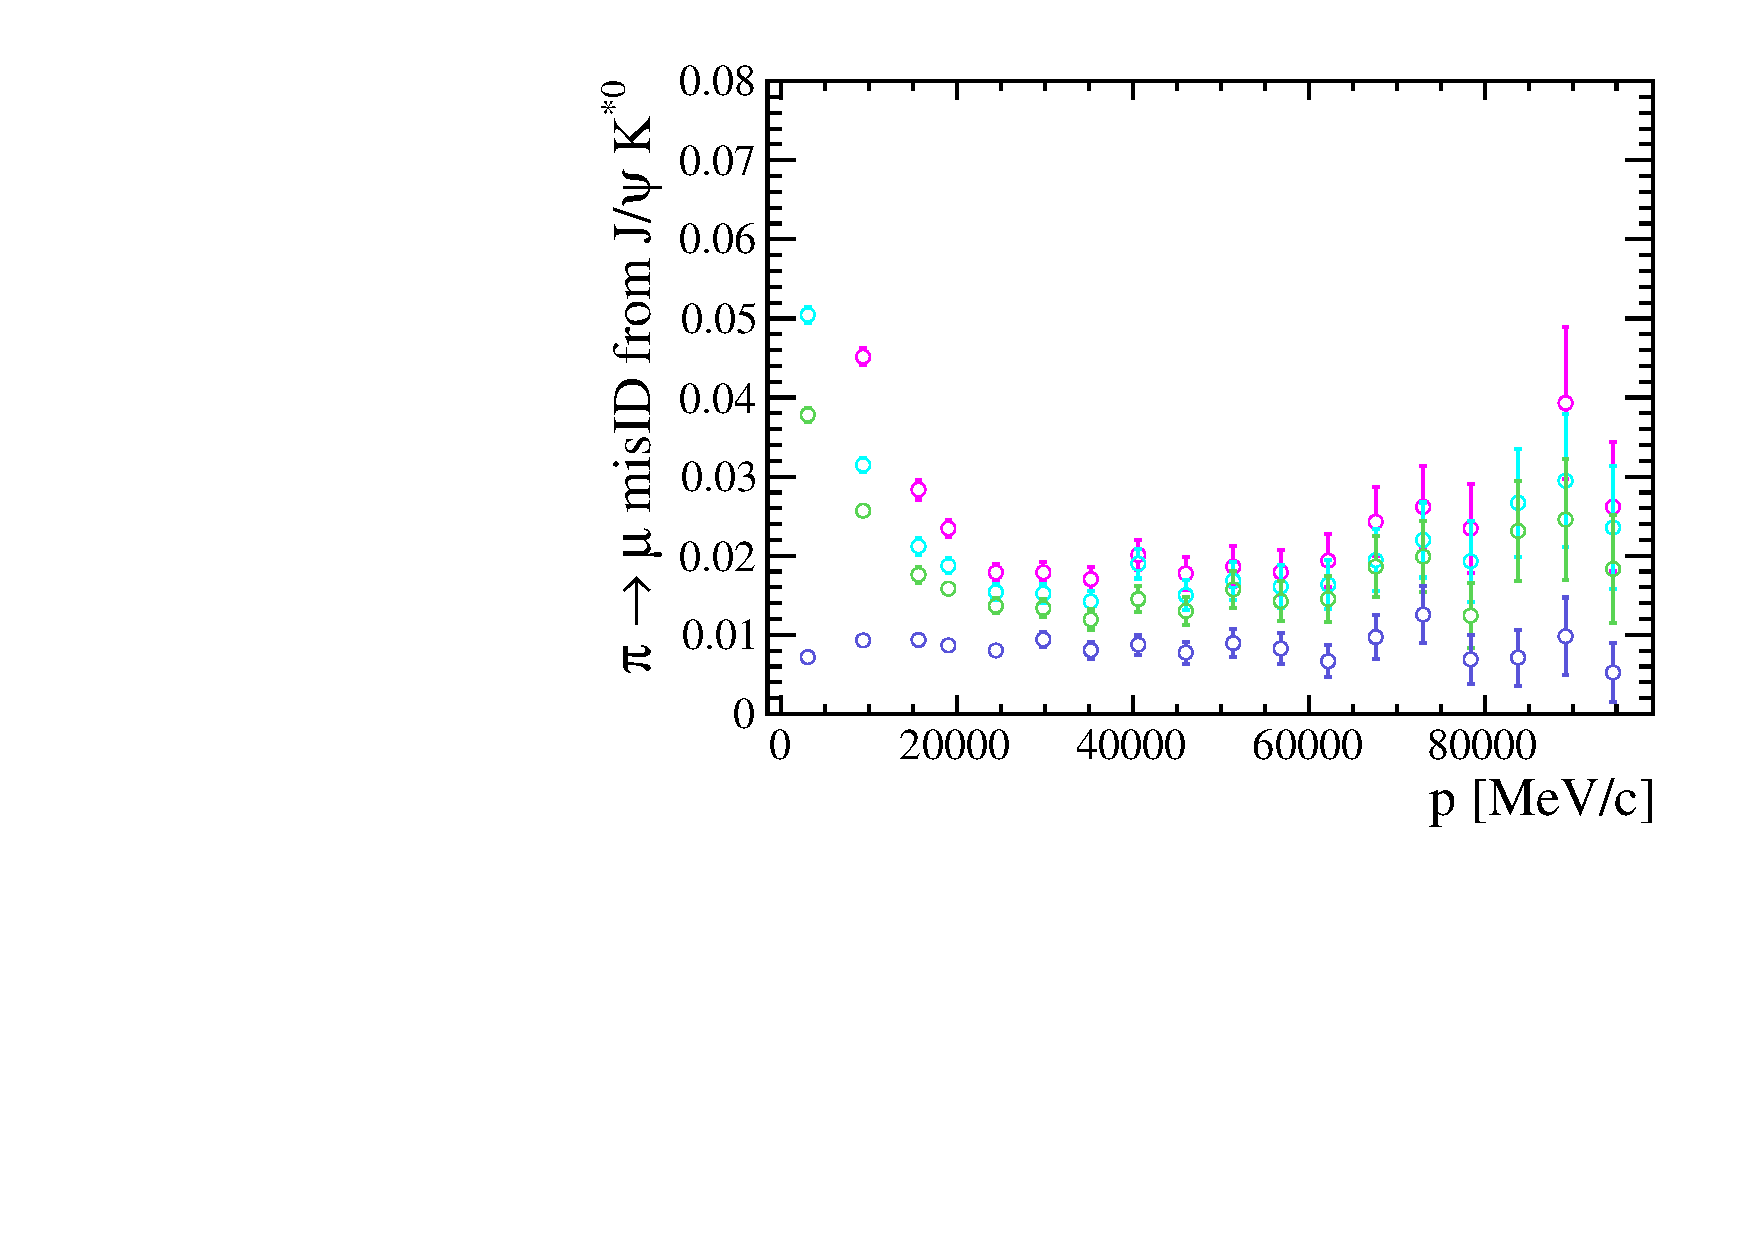
\includegraphics[width = 0.5\textwidth]{figs/trimuon/jpsikst/2016/Visualize_Weights_PionMisid_2016_small_thesis.pdf}\put(-50,133){(a)}
%		\newline
%		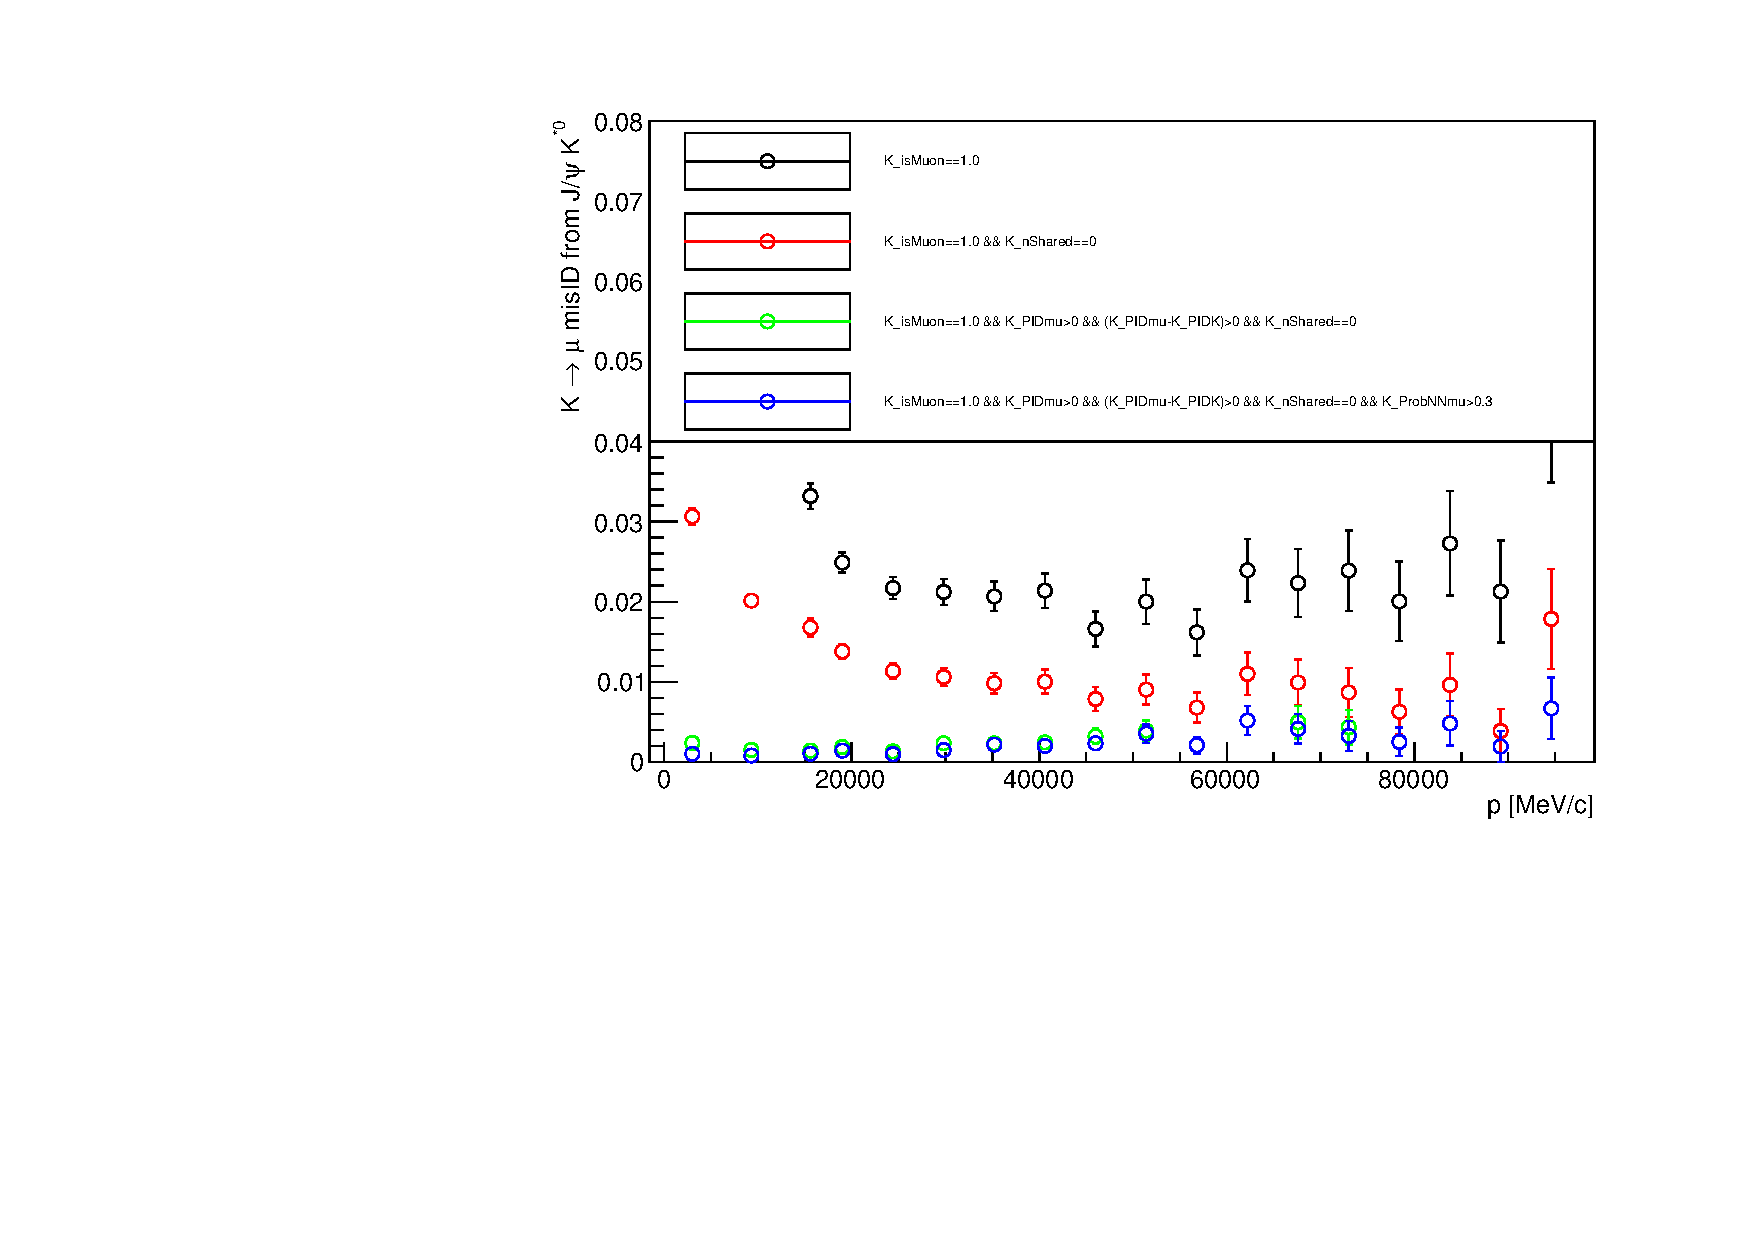
\includegraphics[width = 0.55\textwidth]{figs/trimuon/jpsikst/2012/Visualize_Weights_KaonMisid_small.pdf}\put(-50,133){(c)}%
		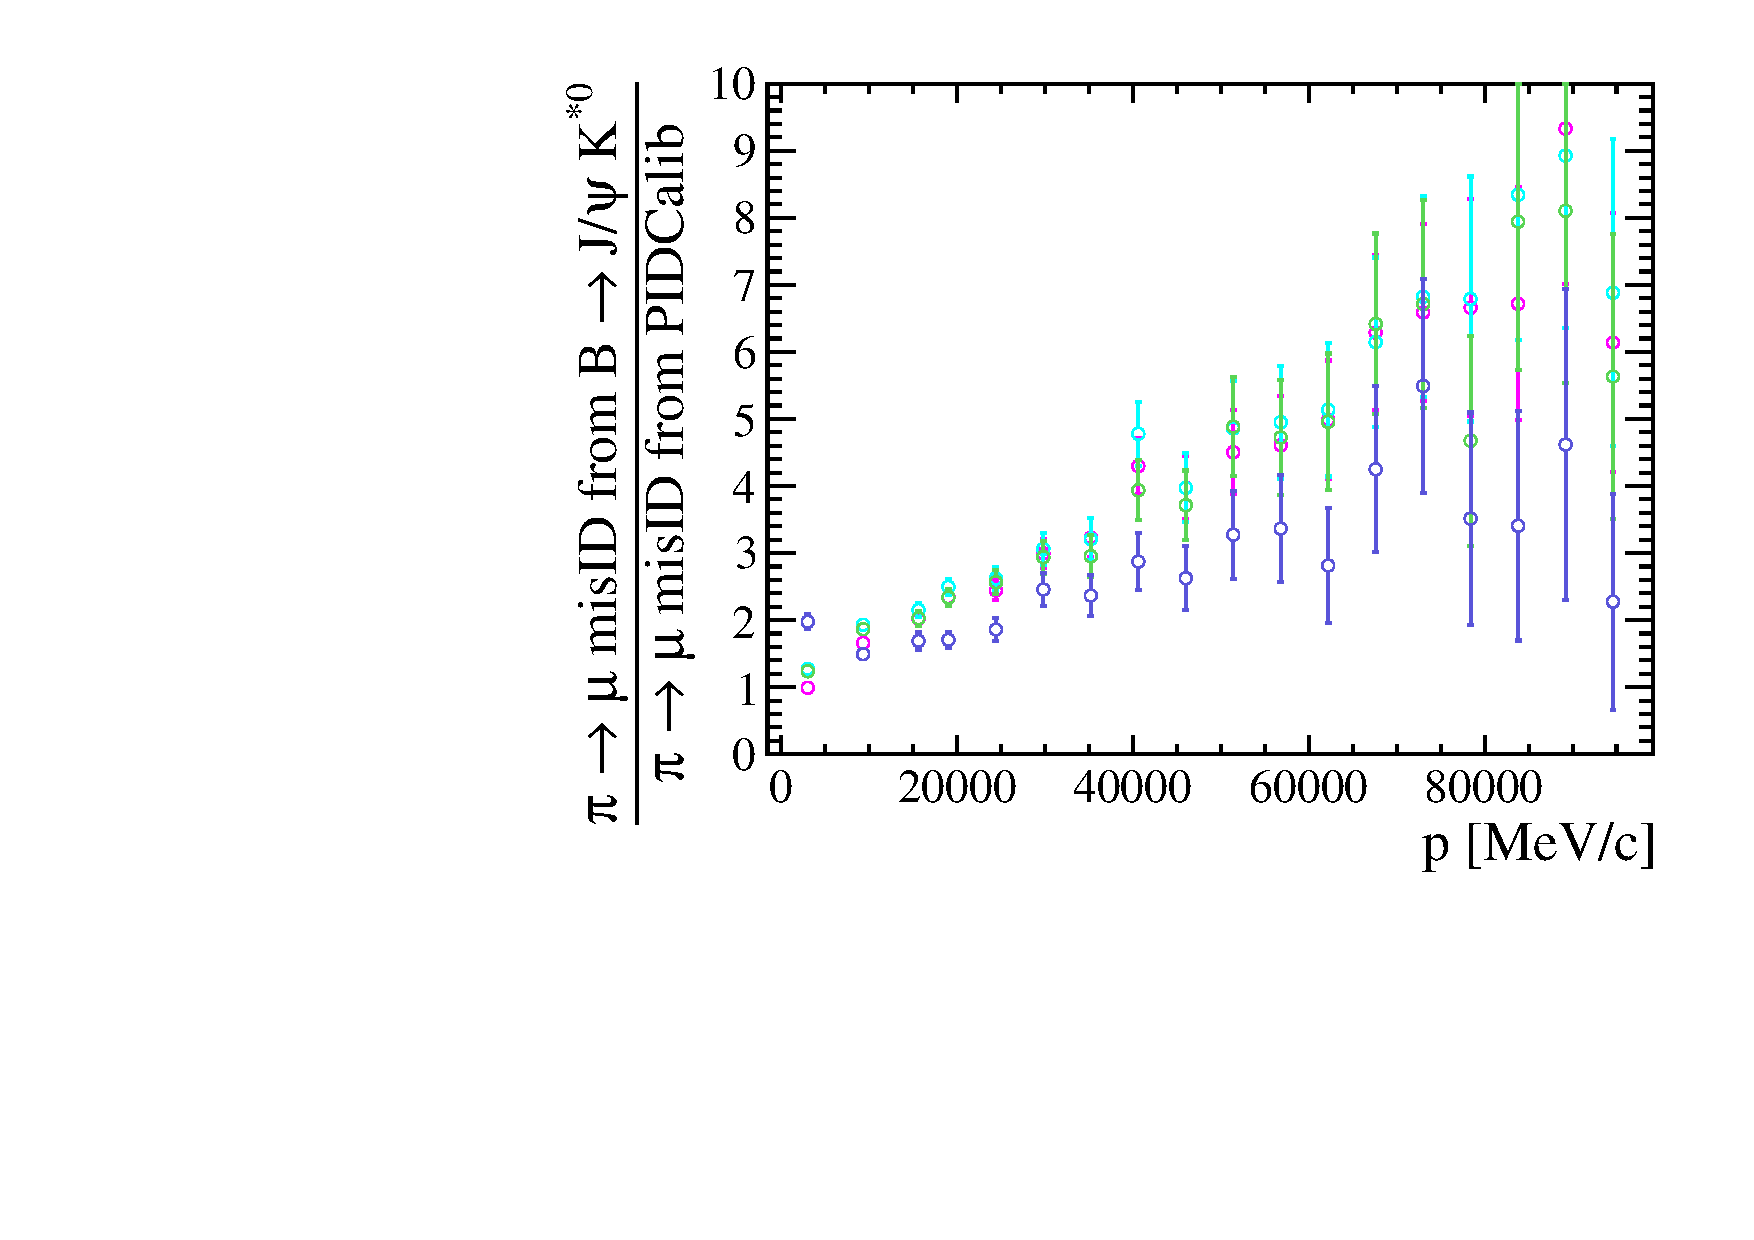
\includegraphics[width = 0.5\textwidth]{figs/trimuon/jpsikst/2016/Visualize_Ratios_PionMisid_2016_small_thesis.pdf}\put(-50,133){(b)}
		\newline
%		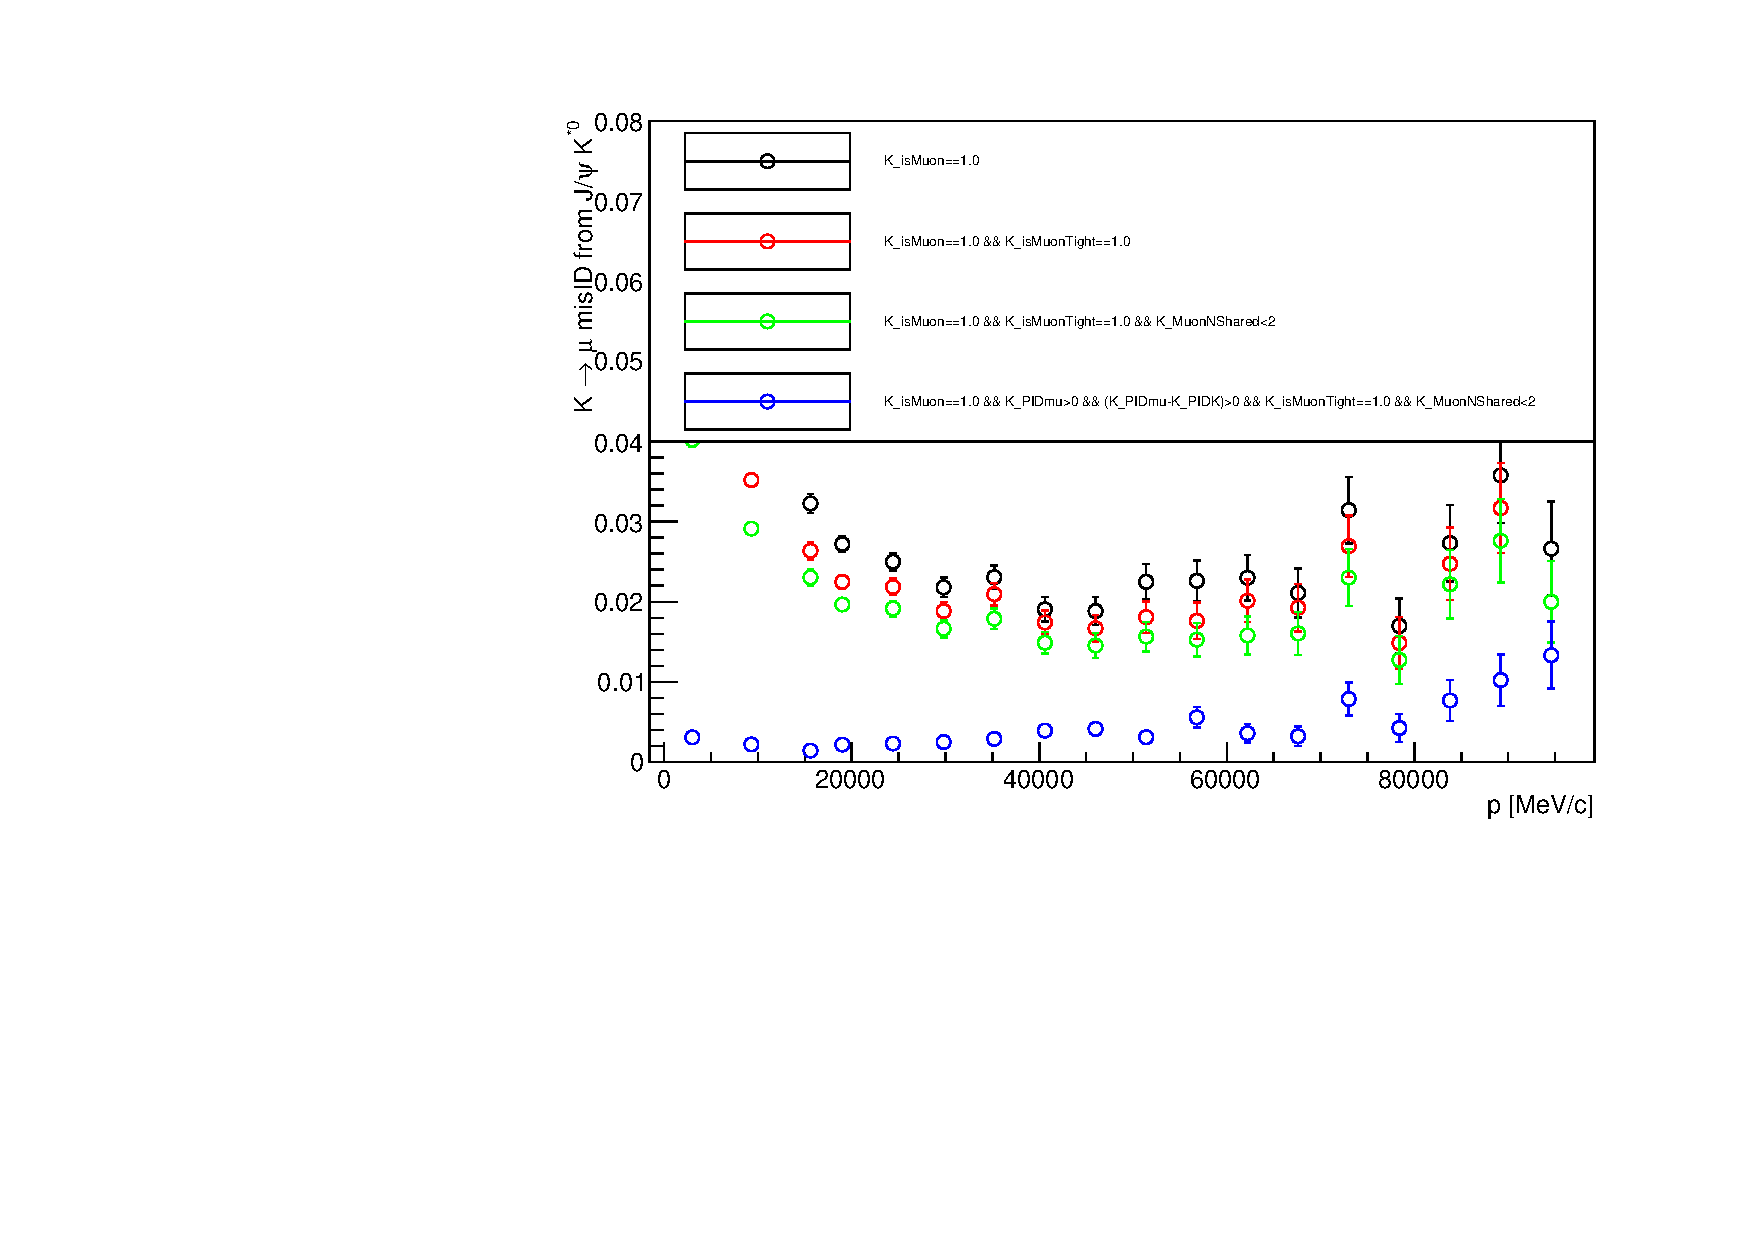
\includegraphics[width = 0.55\textwidth]{figs/trimuon/jpsikst/2012/Visualize_Weights_KaonMisid_2016_small.pdf}\put(-50,133){(e)}%
		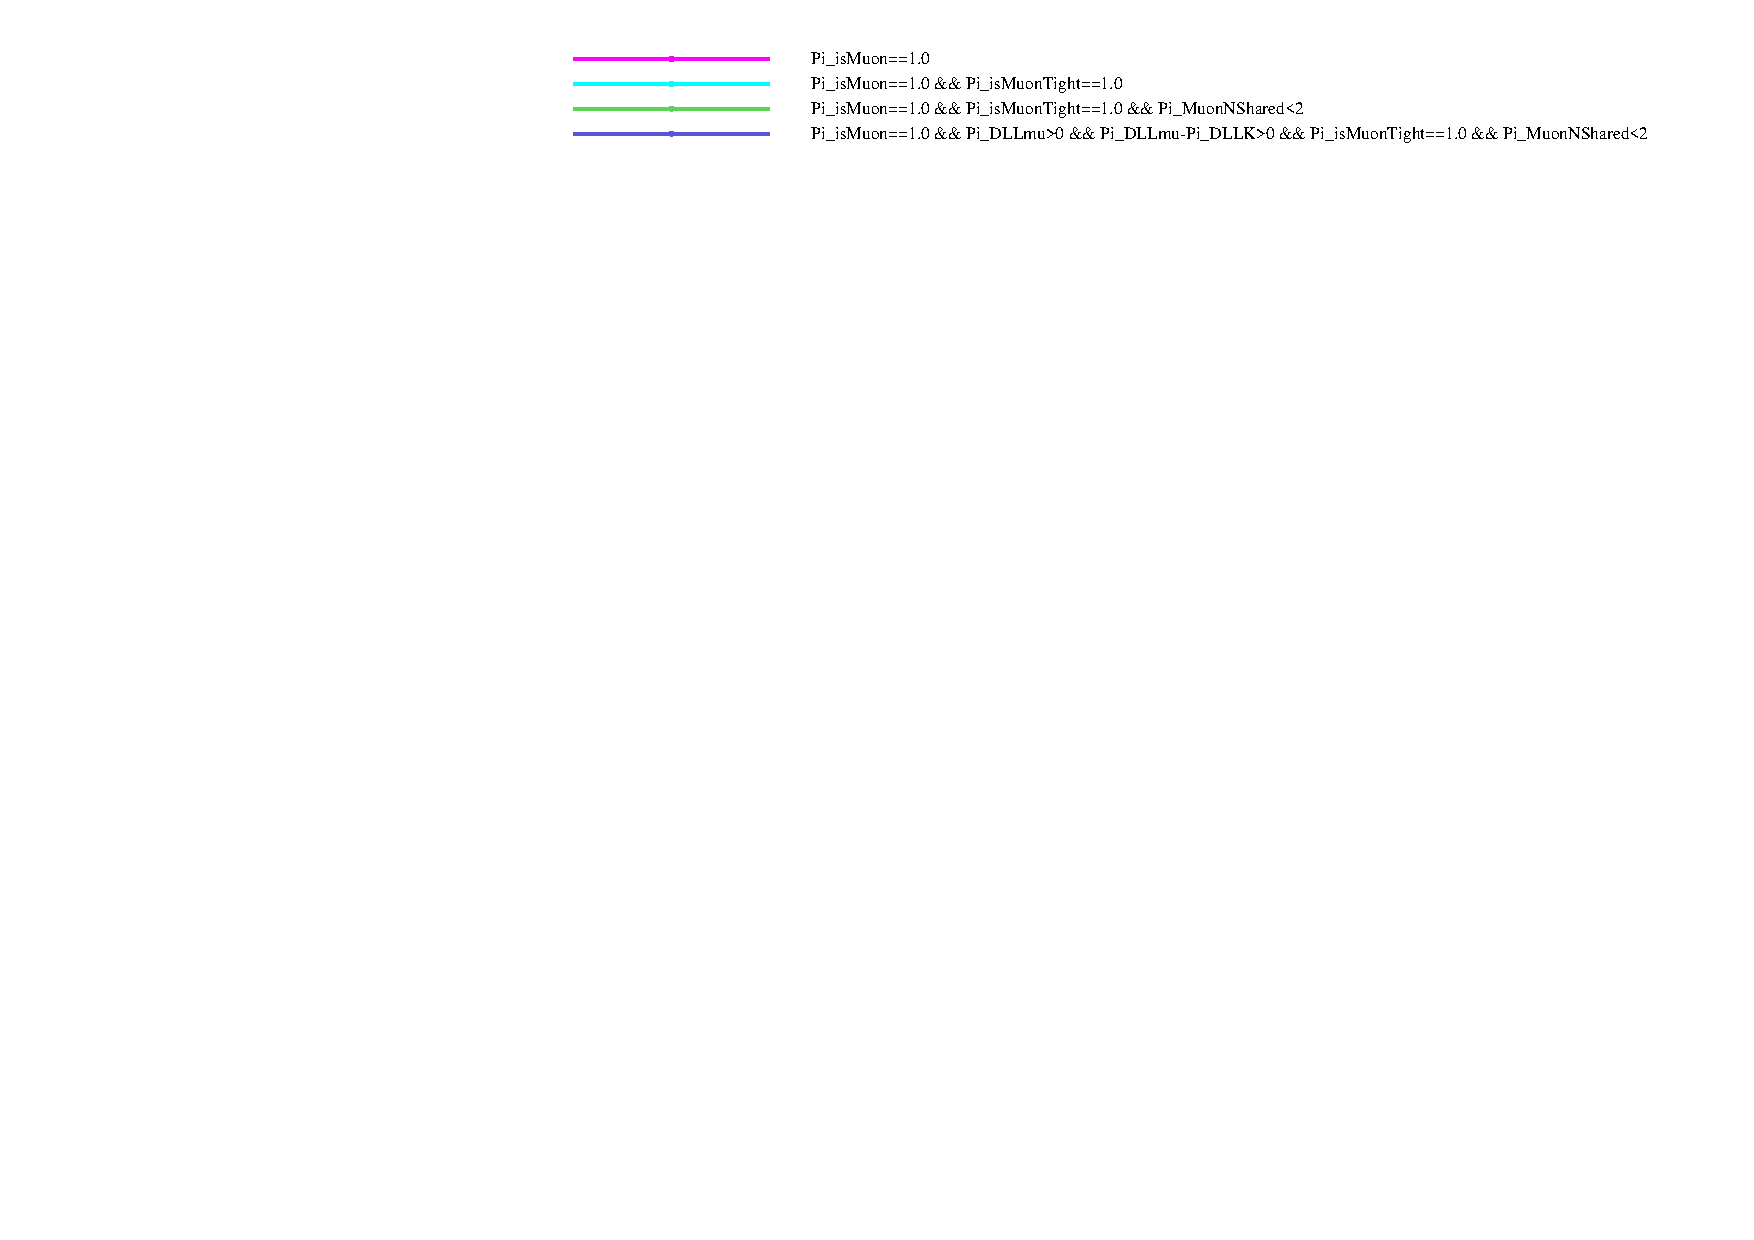
\includegraphics[width = 1.0\textwidth]{figs/trimuon/jpsikst/2016/Visualize_Weights_PionMisid_2016_small_thesis_legend.pdf}
		\caption{(a) $\pi \rightarrow \mu$ misID probabibility for different PID requirements obtained using $B^{0} \rightarrow J/\psi(\rightarrow \mu^{+} \mu^{-}) K^{*} (\rightarrow {K^{+} \pi^{-}} )$ for 2016 data. (b) This is compared to the standard \texttt{PIDCalib} $D^{*+}(\rightarrow D^{0}(\rightarrow K^{+} \pi^{-}) \pi^{+})$ sample. }
		\label{fig:JpsiPionnew2016}
\end{figure}


\begin{figure}[h!]
\center
%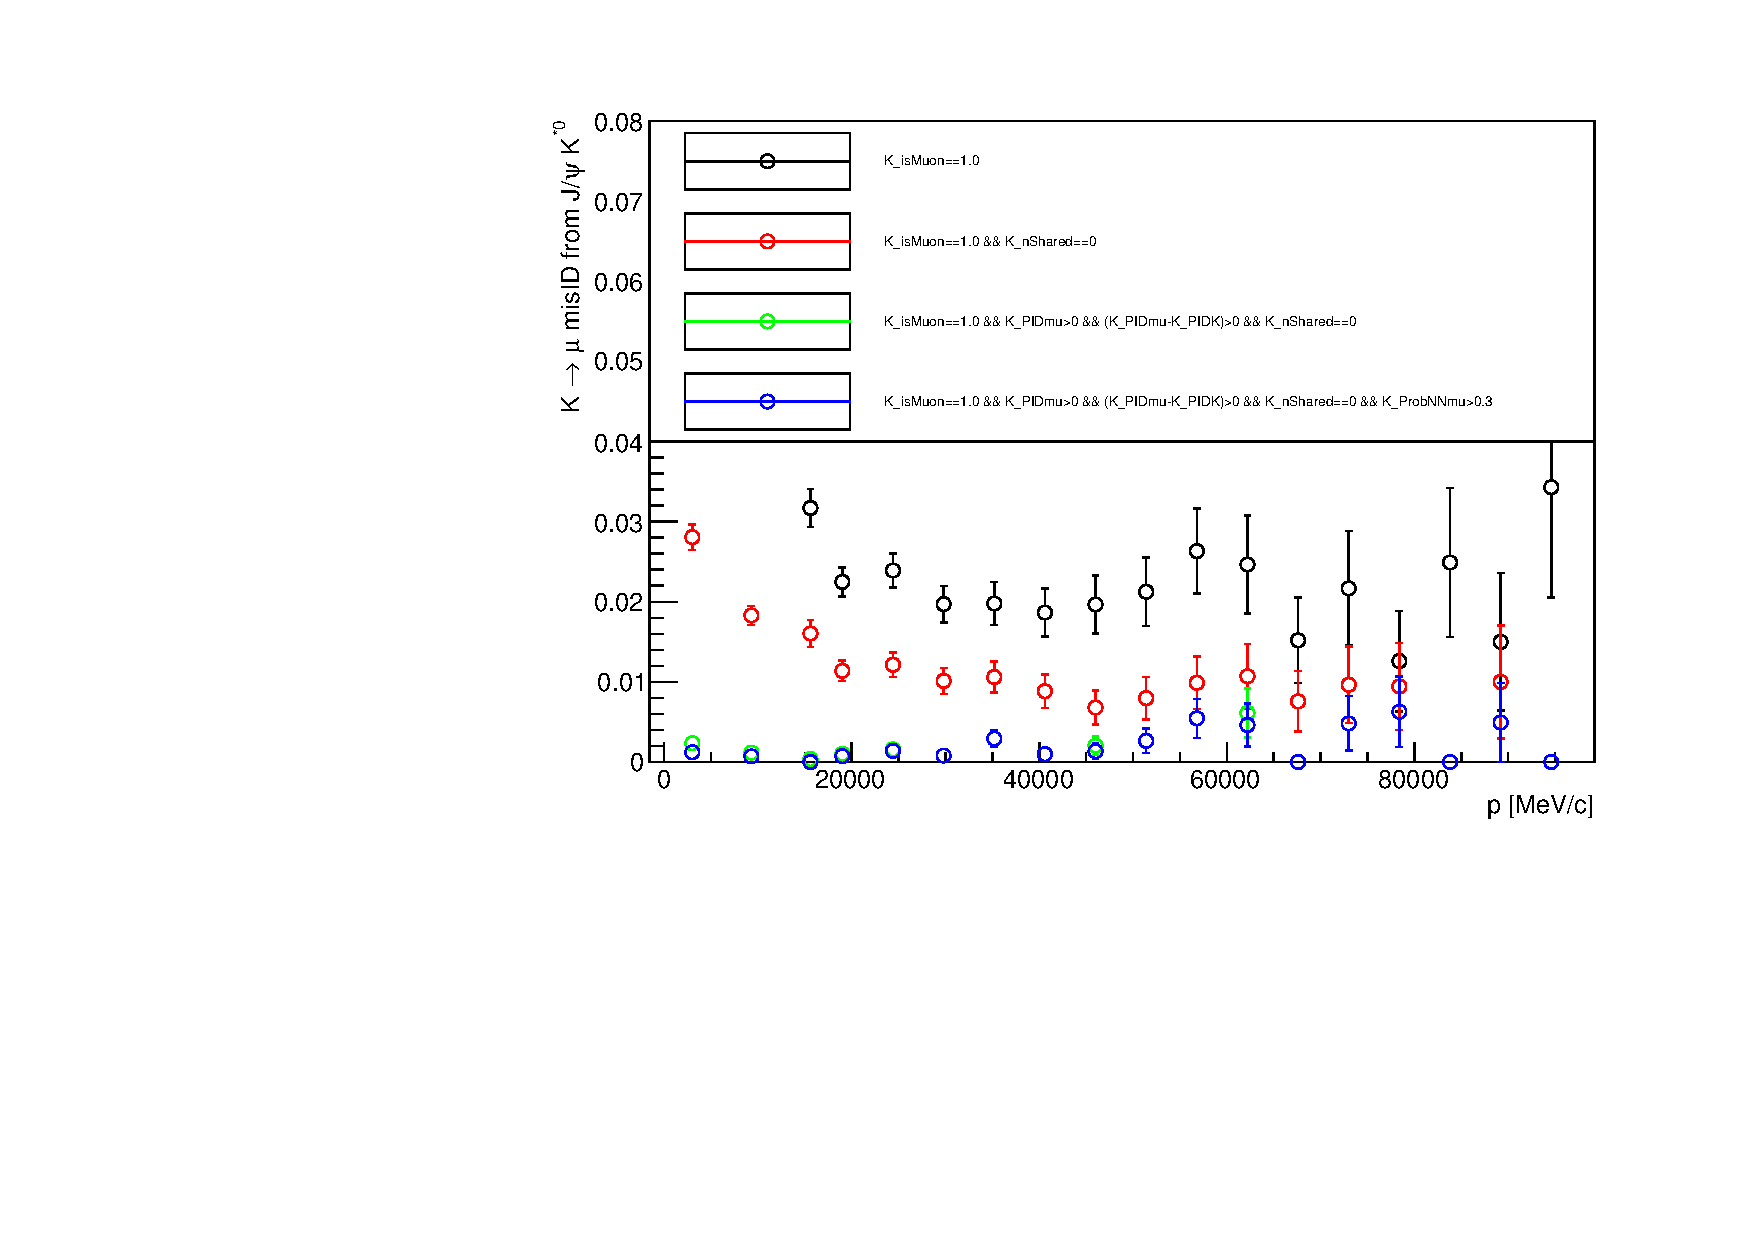
\includegraphics[width = 0.55\textwidth]{figs/trimuon/jpsikst/2012/Visualize_Weights_KaonMisid_2011_small.pdf}\put(-50,133){(a)}%
		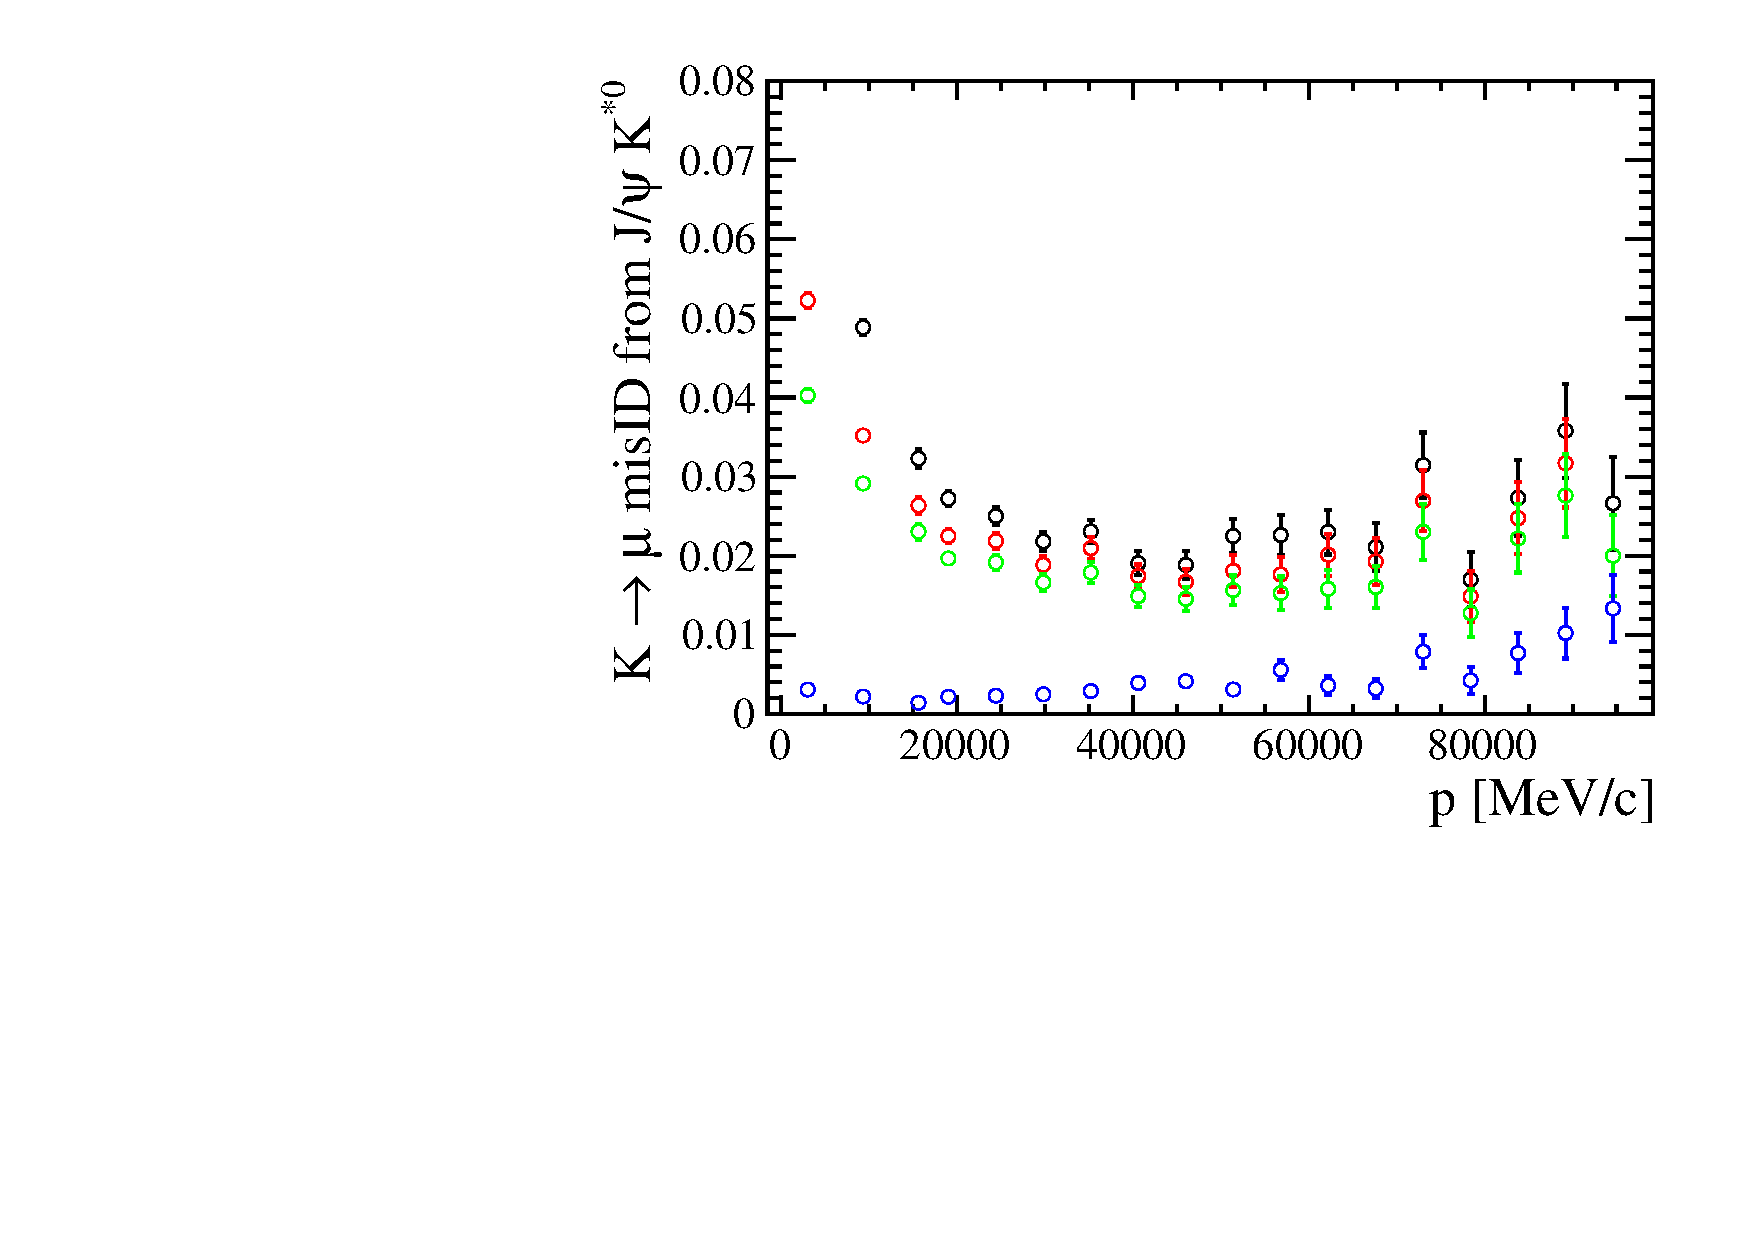
\includegraphics[width = 0.5\textwidth]{figs/trimuon/jpsikst/2016/Visualize_Weights_KaonMisid_2016_small_thesis.pdf}\put(-50,133){(a)}
%		\newline
%		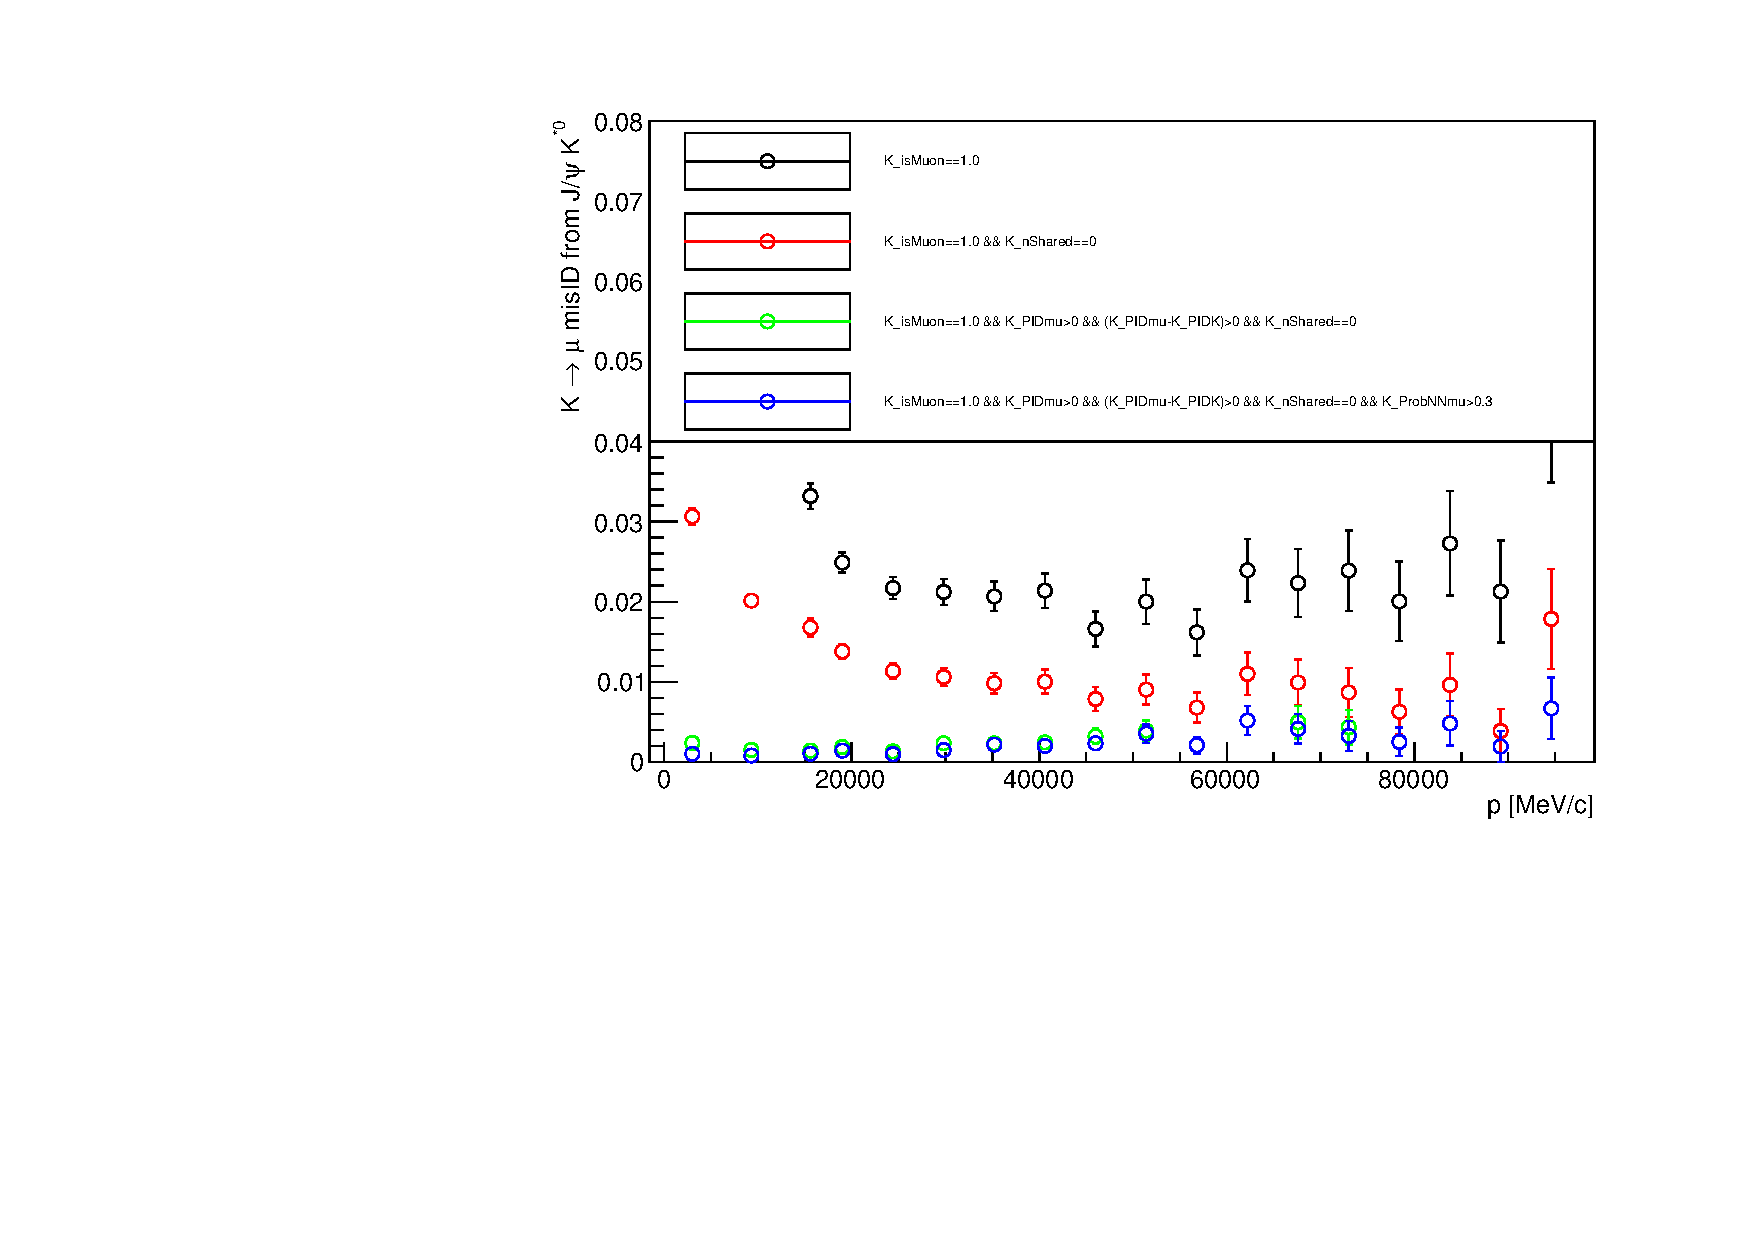
\includegraphics[width = 0.55\textwidth]{figs/trimuon/jpsikst/2012/Visualize_Weights_KaonMisid_small.pdf}\put(-50,133){(c)}%
		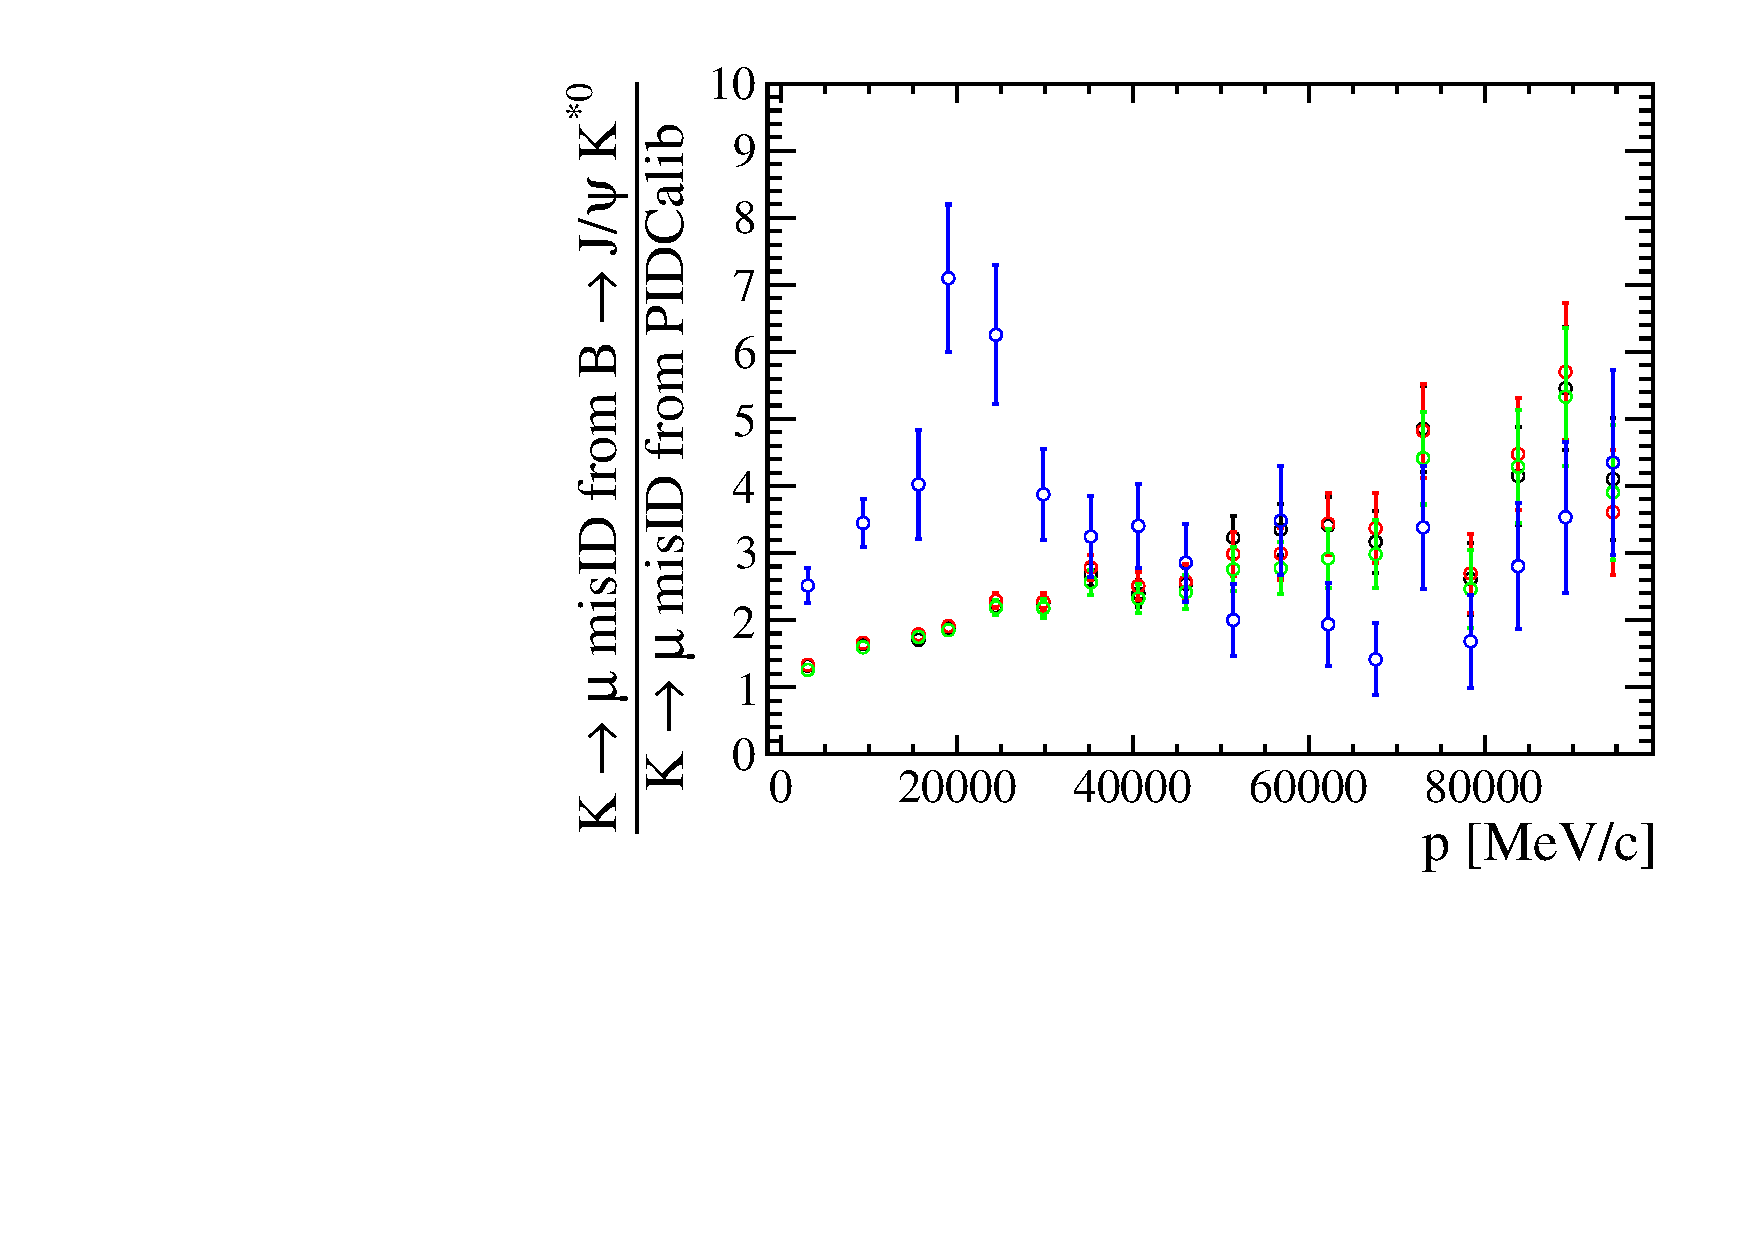
\includegraphics[width = 0.5\textwidth]{figs/trimuon/jpsikst/2016/Visualize_Ratios_2016_KaonMisid_small_thesis.pdf}\put(-50,133){(b)}
		\newline
%		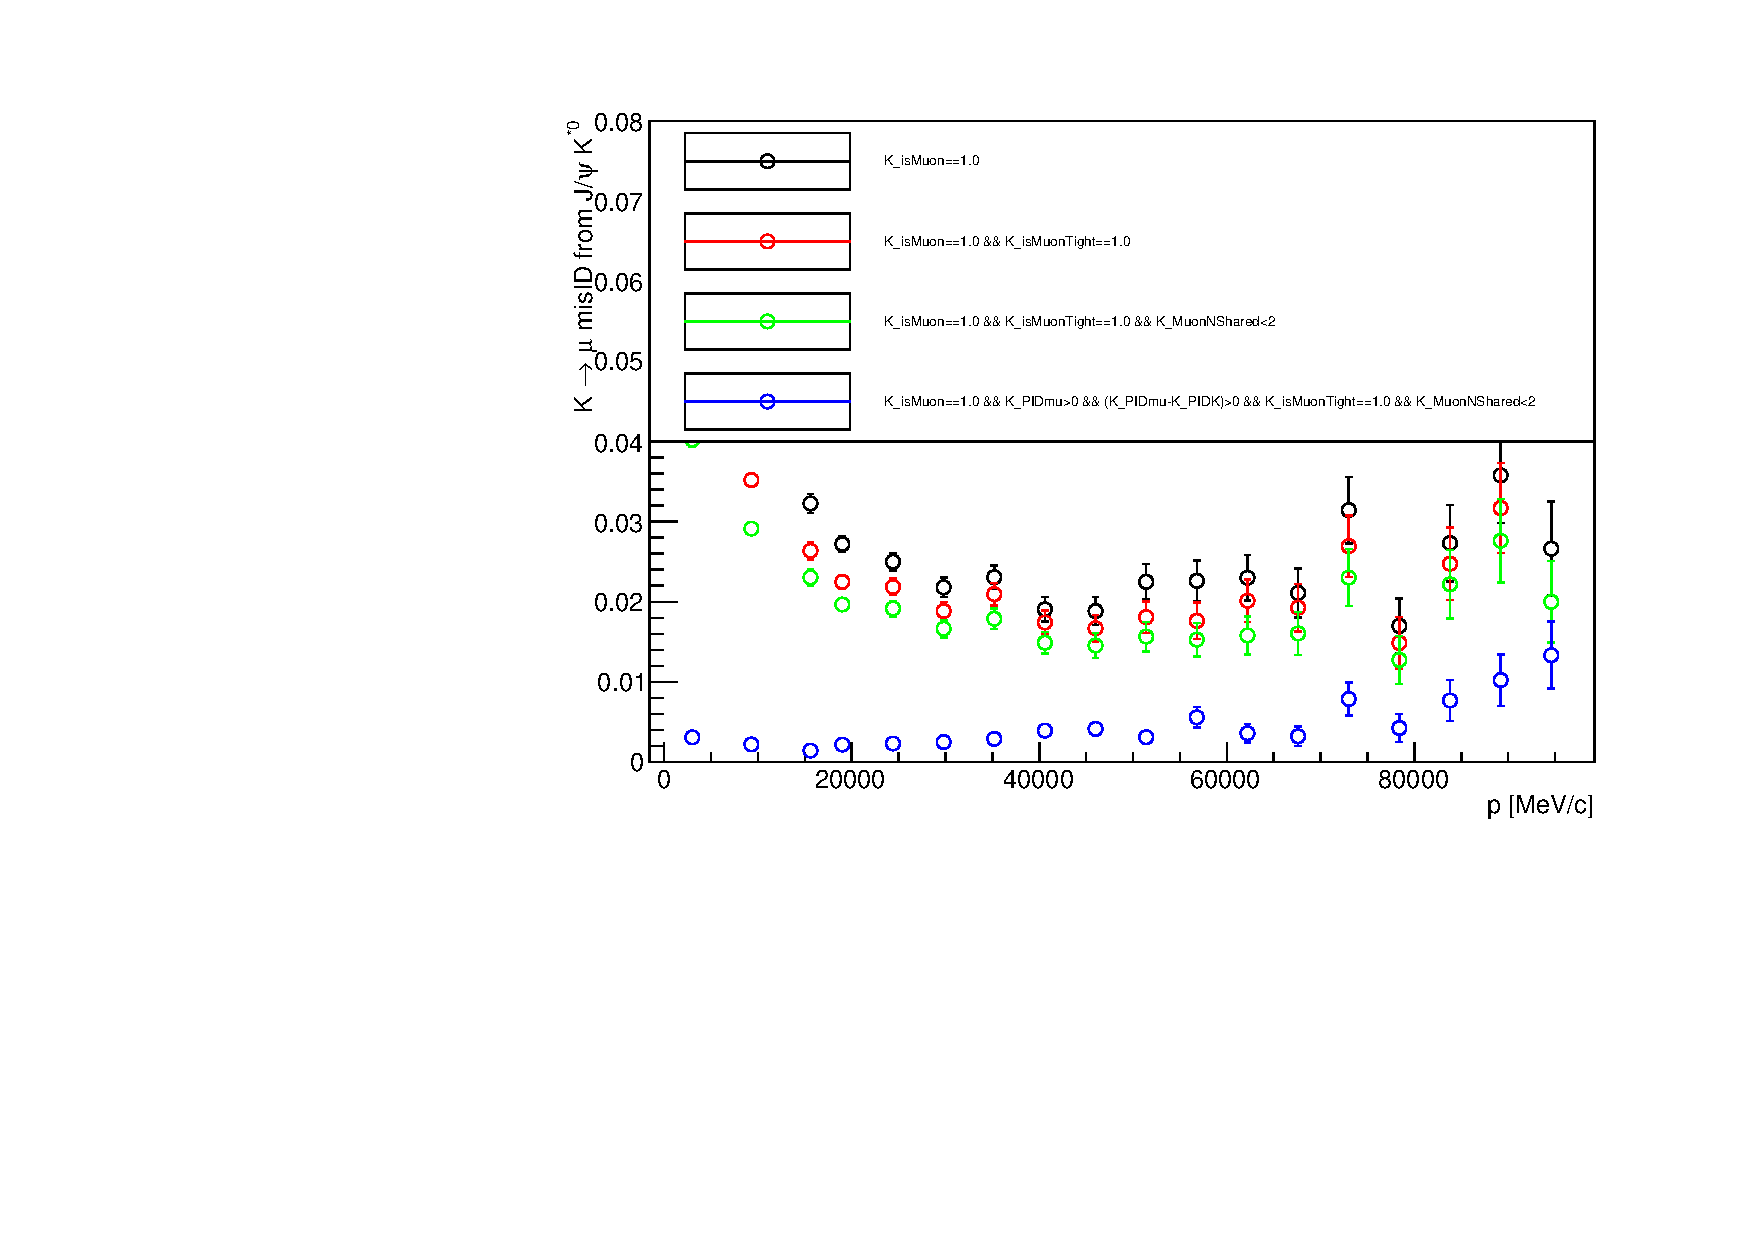
\includegraphics[width = 0.55\textwidth]{figs/trimuon/jpsikst/2012/Visualize_Weights_KaonMisid_2016_small.pdf}\put(-50,133){(e)}%
		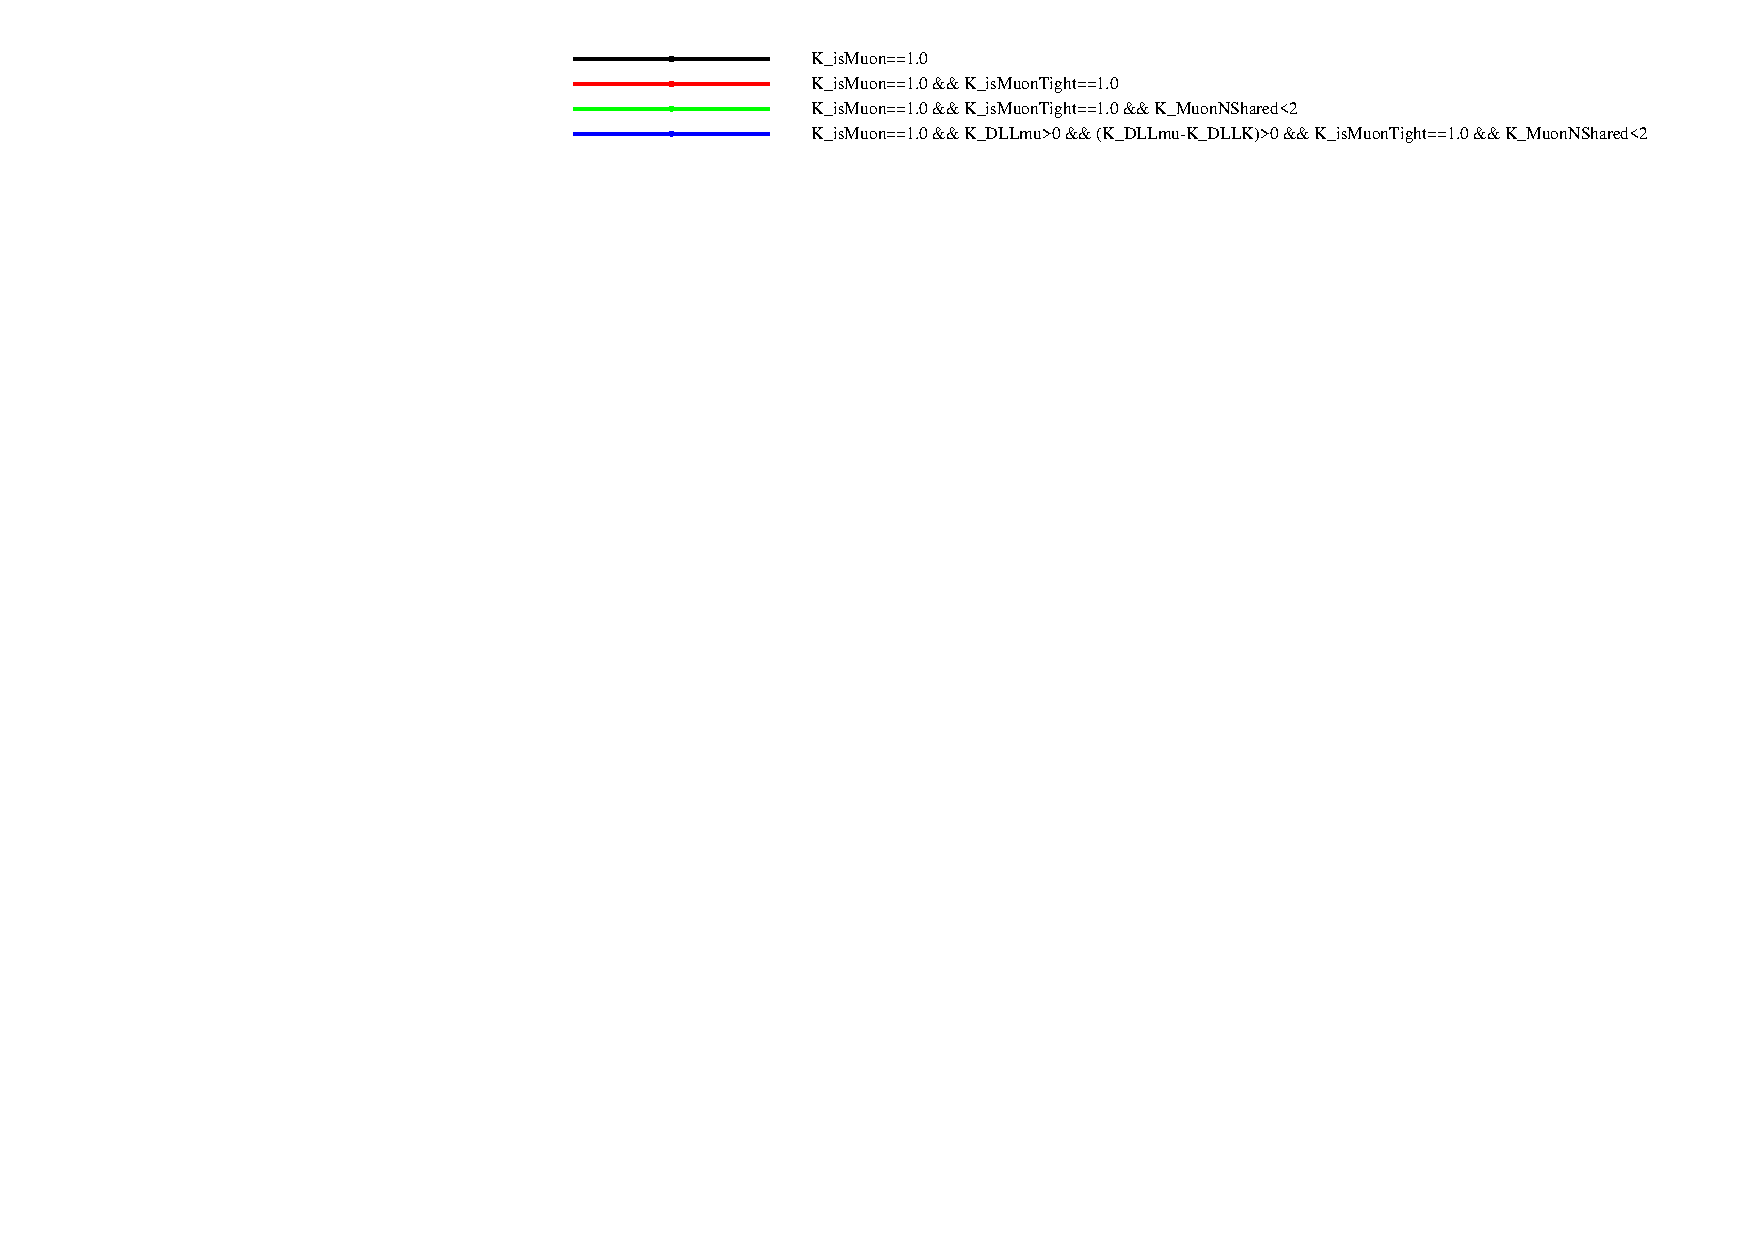
\includegraphics[width = 1.0\textwidth]{figs/trimuon/jpsikst/2016/Visualize_Weights_KaonMisid_2016_small_thesis_legend.pdf}
		\caption{(a) $K \rightarrow \mu$ misID probability for different PID requirements obtained using $B^{0} \rightarrow J/\psi(\rightarrow \mu^{+} \mu^{-}) K^{*} (\rightarrow {K^{+} \pi^{-}} )$ for 2016 data. (b) This is compared to the standard \texttt{PIDCalib} $D^{*+}(\rightarrow D^{0}(\rightarrow K^{+} \pi^{-}) \pi^{+})$ sample. }
		\label{fig:JpsiKaonnew2016}
\end{figure}


